\documentclass[]{book}
\usepackage{lmodern}
\usepackage{amssymb,amsmath}
\usepackage{ifxetex,ifluatex}
\usepackage{fixltx2e} % provides \textsubscript
\ifnum 0\ifxetex 1\fi\ifluatex 1\fi=0 % if pdftex
  \usepackage[T1]{fontenc}
  \usepackage[utf8]{inputenc}
\else % if luatex or xelatex
  \ifxetex
    \usepackage{mathspec}
  \else
    \usepackage{fontspec}
  \fi
  \defaultfontfeatures{Ligatures=TeX,Scale=MatchLowercase}
\fi
% use upquote if available, for straight quotes in verbatim environments
\IfFileExists{upquote.sty}{\usepackage{upquote}}{}
% use microtype if available
\IfFileExists{microtype.sty}{%
\usepackage[]{microtype}
\UseMicrotypeSet[protrusion]{basicmath} % disable protrusion for tt fonts
}{}
\PassOptionsToPackage{hyphens}{url} % url is loaded by hyperref
\usepackage[unicode=true]{hyperref}
\hypersetup{
            pdftitle={R for HR: An Introduction to Human Resource Analytics Using R},
            pdfauthor={David E. Caughlin},
            pdfborder={0 0 0},
            breaklinks=true}
\urlstyle{same}  % don't use monospace font for urls
\usepackage{natbib}
\bibliographystyle{apalike}
\usepackage{color}
\usepackage{fancyvrb}
\newcommand{\VerbBar}{|}
\newcommand{\VERB}{\Verb[commandchars=\\\{\}]}
\DefineVerbatimEnvironment{Highlighting}{Verbatim}{commandchars=\\\{\}}
% Add ',fontsize=\small' for more characters per line
\usepackage{framed}
\definecolor{shadecolor}{RGB}{248,248,248}
\newenvironment{Shaded}{\begin{snugshade}}{\end{snugshade}}
\newcommand{\KeywordTok}[1]{\textcolor[rgb]{0.13,0.29,0.53}{\textbf{#1}}}
\newcommand{\DataTypeTok}[1]{\textcolor[rgb]{0.13,0.29,0.53}{#1}}
\newcommand{\DecValTok}[1]{\textcolor[rgb]{0.00,0.00,0.81}{#1}}
\newcommand{\BaseNTok}[1]{\textcolor[rgb]{0.00,0.00,0.81}{#1}}
\newcommand{\FloatTok}[1]{\textcolor[rgb]{0.00,0.00,0.81}{#1}}
\newcommand{\ConstantTok}[1]{\textcolor[rgb]{0.00,0.00,0.00}{#1}}
\newcommand{\CharTok}[1]{\textcolor[rgb]{0.31,0.60,0.02}{#1}}
\newcommand{\SpecialCharTok}[1]{\textcolor[rgb]{0.00,0.00,0.00}{#1}}
\newcommand{\StringTok}[1]{\textcolor[rgb]{0.31,0.60,0.02}{#1}}
\newcommand{\VerbatimStringTok}[1]{\textcolor[rgb]{0.31,0.60,0.02}{#1}}
\newcommand{\SpecialStringTok}[1]{\textcolor[rgb]{0.31,0.60,0.02}{#1}}
\newcommand{\ImportTok}[1]{#1}
\newcommand{\CommentTok}[1]{\textcolor[rgb]{0.56,0.35,0.01}{\textit{#1}}}
\newcommand{\DocumentationTok}[1]{\textcolor[rgb]{0.56,0.35,0.01}{\textbf{\textit{#1}}}}
\newcommand{\AnnotationTok}[1]{\textcolor[rgb]{0.56,0.35,0.01}{\textbf{\textit{#1}}}}
\newcommand{\CommentVarTok}[1]{\textcolor[rgb]{0.56,0.35,0.01}{\textbf{\textit{#1}}}}
\newcommand{\OtherTok}[1]{\textcolor[rgb]{0.56,0.35,0.01}{#1}}
\newcommand{\FunctionTok}[1]{\textcolor[rgb]{0.00,0.00,0.00}{#1}}
\newcommand{\VariableTok}[1]{\textcolor[rgb]{0.00,0.00,0.00}{#1}}
\newcommand{\ControlFlowTok}[1]{\textcolor[rgb]{0.13,0.29,0.53}{\textbf{#1}}}
\newcommand{\OperatorTok}[1]{\textcolor[rgb]{0.81,0.36,0.00}{\textbf{#1}}}
\newcommand{\BuiltInTok}[1]{#1}
\newcommand{\ExtensionTok}[1]{#1}
\newcommand{\PreprocessorTok}[1]{\textcolor[rgb]{0.56,0.35,0.01}{\textit{#1}}}
\newcommand{\AttributeTok}[1]{\textcolor[rgb]{0.77,0.63,0.00}{#1}}
\newcommand{\RegionMarkerTok}[1]{#1}
\newcommand{\InformationTok}[1]{\textcolor[rgb]{0.56,0.35,0.01}{\textbf{\textit{#1}}}}
\newcommand{\WarningTok}[1]{\textcolor[rgb]{0.56,0.35,0.01}{\textbf{\textit{#1}}}}
\newcommand{\AlertTok}[1]{\textcolor[rgb]{0.94,0.16,0.16}{#1}}
\newcommand{\ErrorTok}[1]{\textcolor[rgb]{0.64,0.00,0.00}{\textbf{#1}}}
\newcommand{\NormalTok}[1]{#1}
\usepackage{longtable,booktabs}
% Fix footnotes in tables (requires footnote package)
\IfFileExists{footnote.sty}{\usepackage{footnote}\makesavenoteenv{long table}}{}
\usepackage{graphicx,grffile}
\makeatletter
\def\maxwidth{\ifdim\Gin@nat@width>\linewidth\linewidth\else\Gin@nat@width\fi}
\def\maxheight{\ifdim\Gin@nat@height>\textheight\textheight\else\Gin@nat@height\fi}
\makeatother
% Scale images if necessary, so that they will not overflow the page
% margins by default, and it is still possible to overwrite the defaults
% using explicit options in \includegraphics[width, height, ...]{}
\setkeys{Gin}{width=\maxwidth,height=\maxheight,keepaspectratio}
\IfFileExists{parskip.sty}{%
\usepackage{parskip}
}{% else
\setlength{\parindent}{0pt}
\setlength{\parskip}{6pt plus 2pt minus 1pt}
}
\setlength{\emergencystretch}{3em}  % prevent overfull lines
\providecommand{\tightlist}{%
  \setlength{\itemsep}{0pt}\setlength{\parskip}{0pt}}
\setcounter{secnumdepth}{5}
% Redefines (sub)paragraphs to behave more like sections
\ifx\paragraph\undefined\else
\let\oldparagraph\paragraph
\renewcommand{\paragraph}[1]{\oldparagraph{#1}\mbox{}}
\fi
\ifx\subparagraph\undefined\else
\let\oldsubparagraph\subparagraph
\renewcommand{\subparagraph}[1]{\oldsubparagraph{#1}\mbox{}}
\fi

% set default figure placement to htbp
\makeatletter
\def\fps@figure{htbp}
\makeatother

\usepackage{booktabs}

\title{R for HR:\\
\emph{An Introduction to Human Resource Analytics Using R}}
\author{David E. Caughlin}
\date{2020-07-30}

\begin{document}
\maketitle

{
\setcounter{tocdepth}{1}
\tableofcontents
}
\chapter*{Preface}\label{preface}
\addcontentsline{toc}{chapter}{Preface}

The \emph{Preface} offers an orientation to this book, foundational
human resource analytics concepts, and the book's raison d'être.

\section{Growth of HR Analytics}\label{hragrowth}

The term \emph{human resource analytics} can mean different things to
different people and to different organizations. Further, human resource
analytics sometimes goes by other names like people analytics, talent
analytics, workforce analytics, and human capital analytics. While some
may argue distinctions between these different names, for this book, I
will treat them as interchangeable synonyms. Moreover, for the purposes
of this book, \textbf{human resource (HR) analytics} refers to the
``process of collecting, analyzing, interpreting, and reporting
people-related data for the purpose of improving decision making,
achieving strategic objectives, and sustaining a competitive advantage''
\citep[p.~34]{baueretal2020}.

The foundation of HR analytics was solidified over a century ago with
the emergence of disciplines like industrial and organizational (I/O)
psychology. In recent decades, advances in information technology and
systems have reduced the time HR professionals spend on transactional
and administrative activities, thereby creating more time and space for
transformational activities that facilitate the realization of strategic
objectives. HR analytics can play a critical role in such
transformational activities, as it can inform HR system design (e.g.,
selection tool selection, validation, and process) and high-stakes
decision making regarding people within the organization.

\begin{figure}
\centering
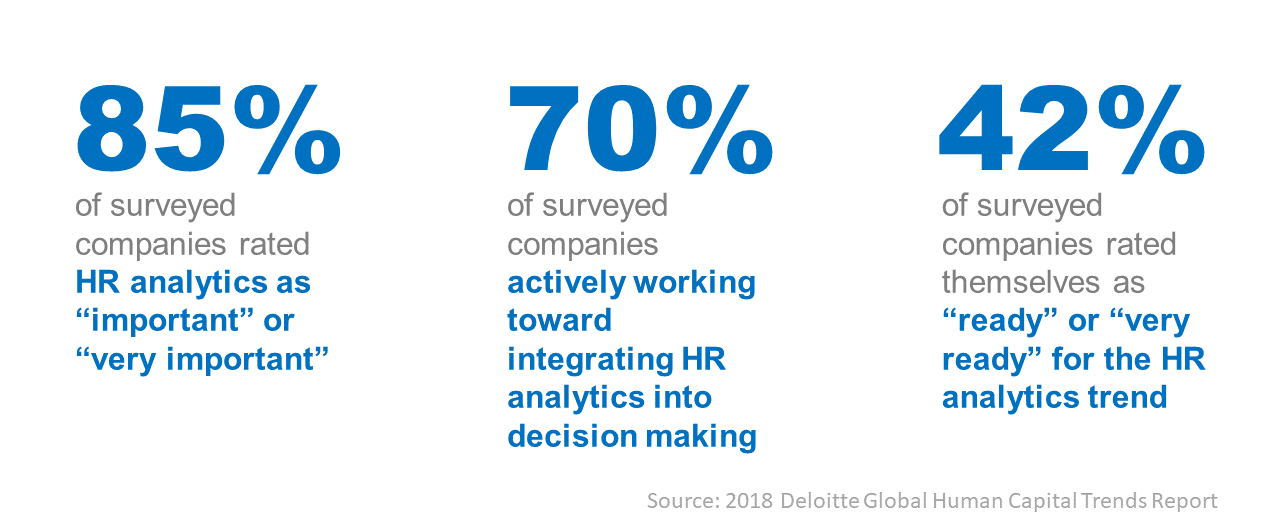
\includegraphics{deloittetrends.png}
\caption{A 2018 survey of companies highlighted the perceived importance
of HR analytics but a relative lack of readiness to adopt and integrate
HR analytics \citep{deloitte2018}.}
\end{figure}

\section{Skills Gap}\label{skills-gap}

Although HR analytics is now widely regarded as strategically important
for organizational success, an HR analytics skills gap has emerged.
Historically, data analytics, data literacy, and numeracy were not major
focal points of academic and industry training for HR professionals,
which has left organizations scrambling to hire new talent or to upskill
existing HR professionals. For some organizations, attempting to fill
the skills gap by hiring a data scientist or statistician may prove
fruitful if the individual works closely with HR professionals who
possess expertise in HR systems, polices, and procedures, as well as
knowledge of legal and ethical considerations that are specific to HR. I
contend, however, that a better alternative is to upskill existing HR
professionals. Presumably, they already possess rich knowledge and
skills related to the HR domain, which can facilitate their ability to
acquire, manage, and analyze data ethically and in line with prevailing
legal guidelines and to interpret and tell a story about the process
that can lead to deployment and implementation of data-informed system
design and practices -- and ultimately to strategic transformation of
the organization and its workforce.

\hypertarget{hraplc}{\section{HR Analytics Project Life
Cycle}\label{hraplc}}

I developed the HR Analytics Project Life Cycle (HRAPLC) as a way to
conceptualize the prototypical phases of a generic project life cycle.
These phases include: (a) Question Formulation, Data Acquisition, Data
Management, Data Analysis, Data Interpretation and Storytelling, and
Deployment and Implementation. This book provides hands-on learning
opportunities for topics and tools related to the Data Acquisition, Data
Management, Data Analysis, and Data Interpretation and Storytelling
phases.

\begin{figure}
\centering
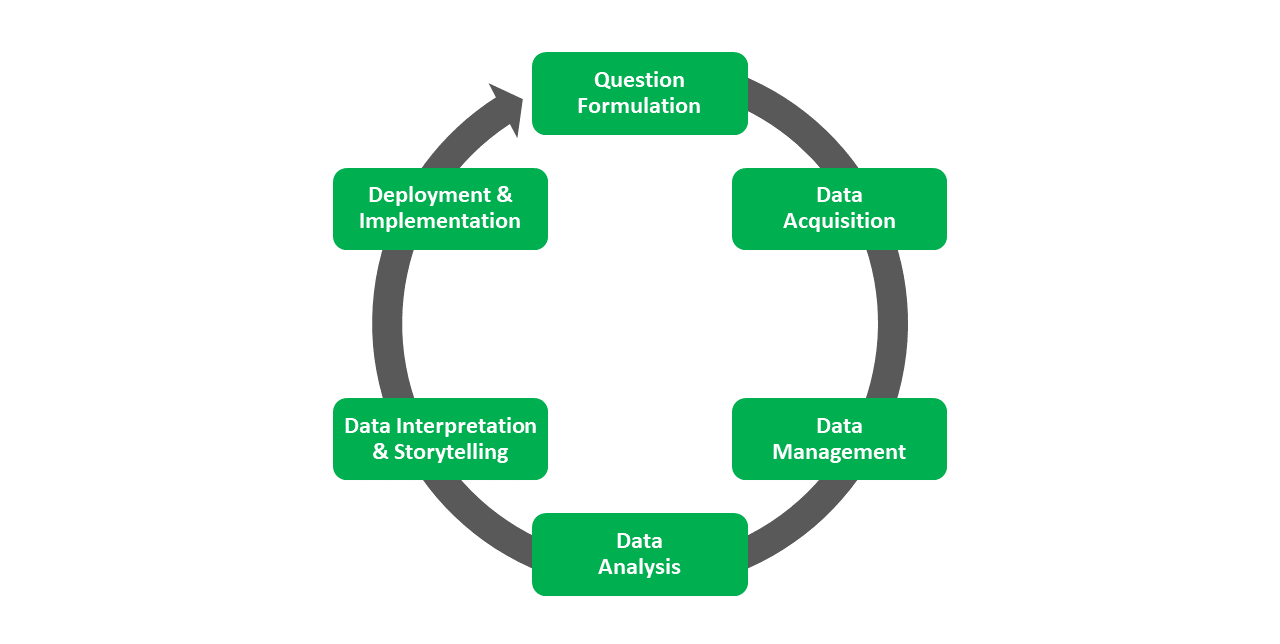
\includegraphics{hraplc.png}
\caption{The Human Resource Analytics Project Life Cycle (HRAPLC) offers
a way to conceptualize the prototypical phases of a generic HR analytics
project life cycle.}
\end{figure}

The phases of the HRAPLC generally align with the generic scientific
process steps of formulating a hypothesis, designing a study, collecting
data, analyzing data, and reporting findings. This highlights how HR
analytics represents a scientific approach to HR management.

\begin{figure}
\centering
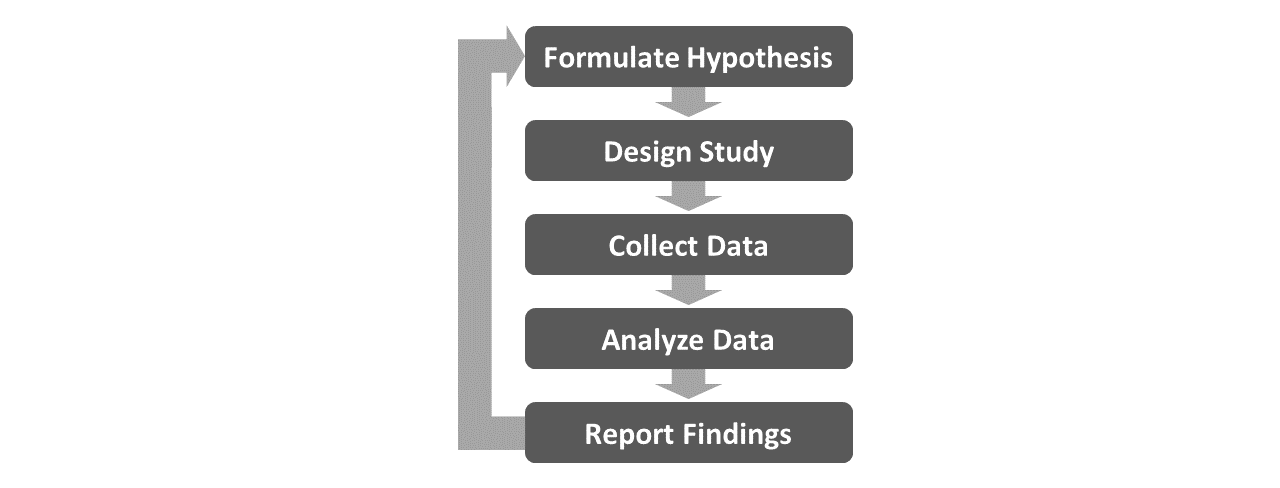
\includegraphics{scientificprocess.png}
\caption{The phases of the Human Resource Analytics Project Life Cycle
(HRAPLC) generally align with steps of the scientific process.}
\end{figure}

\subsection{Question Formulation}\label{questform}

\textbf{Question formulation} refers to the process of posing
strategy-inspired research questions and hypotheses that can be answered
or tested using data. Effective question formulation results in (a)
greater data acquisition, management, and analysis efficiency and (b)
findings that are meaningful to stakeholders.

\hypertarget{dacquire}{\subsection{Data Acquisition}\label{dacquire}}

\textbf{Data acquisition} refers to the process of collecting,
retrieving, gathering, and sourcing data that can be used to answer
questions and test hypotheses. Different tools can be used for data
acquisition, such as employee surveys, (performance) rating forms,
surveillance and monitoring, database queries, and scraping or crawling.
In some instances, the required data may already reside in an HR
information system (HRIS) or enterprise resource planning (ERP)
platform.

\hypertarget{dmanage}{\subsection{Data Management}\label{dmanage}}

\textbf{Data management} refers to the process of wrangling, cleaning,
manipulating, and structuring data. Different tools can be used for data
management, such as database management systems and data analysis
software programs. The general rule of thumb is that you can expect to
spend 80\% of your time managing data and about 20\% of your time
analyzing data.

\hypertarget{danalysis}{\subsection{Data Analysis}\label{danalysis}}

\textbf{Data analysis} refers to the process of applying mathematical,
statistical, and/or computational techniques to data to identify
associations, differences or changes, or classes (categories), as well
as to predict the likelihood of future events, values, or differences or
changes. Various tools used in data analysis, such as mathematics,
statistics, simulations, and computational modeling.

\hypertarget{dinterpret}{\subsection{Data Interpretion \&
Storytelling}\label{dinterpret}}

\textbf{Data interpretation and storytelling} refers to the process of
making sense of data analysis findings and evaluating questions and
hypotheses, as well as disseminating the findings to different
stakeholders. To support interpretation and storytelling, data
visualization is frequently used (e.g., graphs, charts, plots).

\subsection{Deployment \& Implementation}\label{ddeploy}

\textbf{Deployment and implementation} refers to the process of
prescribing or taking action based on interpretation of data-analysis
findings. This phase requires an (a) understanding of stakeholder needs,
(b) an understanding of the business context, and (c) knowledge of
change management theories and practices.

\section{My Philosophy for This Book}\label{philosophy}

Working with data does not need to be scary or intimidating; yet, over
the years, I have interacted with students and professionals who carry
with them what I refer to as a \emph{numerical phobia} or
\emph{quantitative trauma}. Unfortunately, at some point in their lives,
some people are made to believe that they are not suited for
mathematics, statistics, and/or generally working with data. Given these
mental barriers, a primary objective of this book is to make data
analytics -- and HR analytics specifically -- relevant, accessible, and
maybe even a little fun. In early chapters, my intention is to ease the
reader into foundational concepts, applications, and tools in order to
incrementally build self-efficacy in HR analytics. Each chapter is
grounded in a what I hope will be a meaningful context for those who
work in HR or who, at the very least, have some familiarity with the
function and how it relates to the business. As the book progresses,
more challenging statistical concepts and data-analytic techniques are
introduced. Reading this book and following along with the in-chapter
tutorials will not lead to expert-level knowledge and skill; however, my
hope is that completing all or portions of this book will do the
following:

\begin{enumerate}
\def\labelenumi{\arabic{enumi}.}
\tightlist
\item
  Build excitement for working with data to inform decision making.
\item
  Instill a sense of intellectual curiosity about data and a hunger to
  expand boundaries of expertise.
\item
  Inspire further in-depth training, education, and learning in areas
  and topics introduced in this book.
\item
  Enhance data literacy, including knowledge and skills related to (a)
  critical thinking and logic, (b) mathematics, statistics, and data
  analysis, and (c) data visualization and storytelling with data.
\end{enumerate}

\subsection{Rationale for Using R}\label{rationalerpref}

Today, we have the potential to access and use a remarkable number of
statistical and data-analytic programs. Examples of programs and
languages with such capabilities include (in no particular order) R,
Python, SPSS, SAS, Stata, MatLab, Mplus, Tableau, PowerBI, and Microsoft
Excel. Some of these programs can be quite expensive when it comes to
lifetime or annual user licensing costs, which can be a barrier to
access for many.

Programming languages like R and Python have several desirable qualities
when it comes to managing, analyzing, and visualizing data. Namely, both
are free and both have an ever-growing number of free (add-on) packages
with domain- or area-specific functions (e.g., data visualizations). It
is beyond the scope of this \emph{Preface} to provide an exhaustive
comparison of the relative merits of R versus Python; however, when it
comes to the statistical analysis of data, specifically, I argue that R
provides a more user-friendly entry point for beginners as well as more
advanced capabilities desired by expert users. Moreover, the integrated
development environment program called RStudio (which ``sits on top
of''" base R) offers useful workflow tools and generally makes for an
inviting environment within which the R engine can be run.

With all that said, Python has been catching up in these regards, and I
wouldn't be surprised if Python closes these gaps relative to R in the
next few years. I would be remiss if I didn't mention that the Python
language is powerful and has capabilities that extend far beyond the
management, analysis, and visualization of data. Fortunately, learning R
makes learning Python easier (and vice versa), which means that this
book can serve as springboard for learning Python or other programming
languages. Finally, I believe it to be unlikely that one program or
language will emerge that is ideal for every task, and thus, I encourage
people to build familiarity with multiple tools so that the best (or at
least better) tool can be used for each task.

\subsection{Audience}\label{audiencepref}

I have written this book with current or soon-to-be HR professionals in
mind, particularly those who have an interest in upskilling their
data-analytic knowledge and skills. With that said, I believe this book
can provide a meaningful context for learning key data-analytic
concepts, applications, and tools that are applicable beyond the HR
context. Relatedly, this book may serve as a gateway to a user-friendly
introduction to the programming language called R.

\subsection{Structure}\label{structurepref}

This book consists of six parts:

\begin{enumerate}
\def\labelenumi{\arabic{enumi}.}
\tightlist
\item
  Introduction
\item
  Data Acquisition
\item
  Data Management
\item
  Data Analysis \& Visualization
\item
  References
\item
  Additional Topics
\end{enumerate}

\subsubsection{Introduction}\label{introductionpref}

The \emph{Introduction} (Part 1) introduces the reader to area of HR
analytics and the R programming language. This part also focuses on how
to install and get started with R and RStudio, including a gentle
introduction to foundational concepts and operations associated with the
R language.

\subsubsection{Data Acquisition}\label{dataacquirepref}

\emph{Data Acquisition} (Part 2) focuses on how to bring data into the R
environment that have been acquired -- and how to export data outside of
the R environment. \protect\hyperlink{dacquire}{Data Acquisition} is a
key phase of the \protect\hyperlink{hraplc}{HR Analytics Project Life
Cycle}.

\subsubsection{Data Management}\label{datamanagepref}

\emph{Data Management} (Part 3) provides an overview to foundational
data management concepts and techniques, such as arranging (sorting),
joining (merging), manipulating (wrangling), aggregating, and cleaning.
\protect\hyperlink{dmanage}{Data Management} is a key phase of the
\protect\hyperlink{hraplc}{HR Analytics Project Life Cycle}.

\subsubsection{Data Analysis \& Visualization}\label{dataanalvizpref}

\emph{Data Analysis \& Visualization} (Part 4) acts as the heart of this
book, as it introduces various mathematical and statistical concepts as
they relate to specific functional areas of HR (e.g., selection,
training). To facilitate the interpretation and communication of
data-analysis findings, various data visualization displays are
showcased. This part integrates the \protect\hyperlink{danalysis}{Data
Analysis} and \protect\hyperlink{dinterpret}{Data Interpretation and
Storytelling} phases of the \protect\hyperlink{hraplc}{HR Analytics
Project Life Cycle}.

\subsubsection{References}\label{ref}

The \emph{References} (Part 5) lists the references for the sources that
are cited throughout the book.

\subsubsection{Additional Topics}\label{addtopicspref}

The \emph{Additional Topics} (Part 6) provides a home to ``else'' -- or
rather, topics that would not fit neatly into Parts 1-4 of the book.
Examples of such topics include question formulation and HR information
systems.

\section{About the Author}\label{aboutauthor}

David Caughlin works for Portland State University's School of Business
where he engages in research and teaching on topics related to
organizational behavior, human resource management, and data analytics.
David received his B.S. in psychology and B.A. in Spanish from Indiana
University, his M.S. in industrial \& organizational psychology from
Indiana University - Purdue University at Indianapolis, and his Ph.D.~in
industrial \& organizational psychology from Portland State University
with concentrations in quantitative methodology and occupational health
psychology. His research interests are generally focused on supervisor
support, work motivation, and occupational safety and health. His
research has been published in peer-reviewed outlets such as
\emph{Journal of Applied Psychology}, \emph{Human Resource Management},
\emph{Journal of Occupational Health Psychology}, and \emph{Psychology,
Public Policy, and the Law}. He co-authored the textbooks \emph{Human
Resource Management: People, Data, and Analytics} and \emph{Fundamentals
of Human Resource Management: People, Data, and Analytics}. In the
School of Business, David teaches undergraduate and graduate courses on
topics related to human resource management, information systems, and
data analytics. In his HR analytics courses, David teaches students how
to apply the statistical programming language R to manage, analyze, and
visualize HR data to improve strategic decision making; in the process,
students build their data literacy and develop their critical-thinking
and reasoning skills. He has received the following teaching awards from
the School of Business: Teaching Innovation Award (2018), ``Extra Mile''
Teaching Excellence Award (2019), and Teaching Innovation Award (2020).
In his free time, David enjoys outdoor activities like trail running,
skiing, mountain biking, and paddle boarding.

\section{Acknowledgements}\label{acknowpref}

My inspiration for writing and compiling the contents of this book stems
from interactions with countless colleagues, professional acquaintances,
and undergraduate and graduate students, and a broad ``thank you'' is in
order for anyone with whom I have taught or had a conversation about HR
analytics specifically or data analytics in general. Finally, I created
this book using the following programs and packages: R \citep{R-base},
RStudio \citep{rstudio2020}, \texttt{rmarkdown}
\citep{rmarkdown2018, R-rmarkdown}, \texttt{knitr}
\citep{knitr2015, knitr2014, R-knitr}, and \texttt{bookdown}
\citep{bookdown2016, R-bookdown}.

\part{Introduction}\label{part-introduction}

\chapter{Installing R \& RStudio}\label{install}

If you have a Windows, Mac, or Linux operating system, you have several
ways in which you can begin working in R. Commonly, users install R on
their computer along with an integrated development environment (IDE)
software application like RStudio. Recently, RStudio Cloud
(\url{https://rstudio.cloud}) has emerged as an alternative to
installing R and RStudio by allowing users to use R and RStudio via the
cloud, which has the advantage of allowing access to R and RStudio when
using the Chrome operating system.

\subsubsection{Video Tutorial}\label{video-tutorial}

Link to video tutorial: \url{https://youtu.be/b18IHQERT4A}.

\section{Downloading \& Installing R}\label{downloading-installing-r}

In the following sections, you will learn how to download and install
the R program for Windows and Mac operating systems. The base R program
must be installed prior to installing the RStudio program. R is
open-source software and free to download.

\subsection{For Windows Operation
Systems}\label{for-windows-operation-systems}

R can currently run under operating systems as old as Windows Vista
(circa 2007). To download R for your Windows operating system for the
first time, click on this link:
\url{https://cran.r-project.org/bin/windows/base/}. Once you are on the
R download page, click on the hyperlink to download the current version
of R for Windows. Once the file has downloaded, follow the installation
prompts.

\subsection{For Mac Operating Systems}\label{for-mac-operating-systems}

The current version of R works with Mac OS X (release 10.6 and higher).
To download R for Mac OS X operating system for the first time, click on
this link: \url{https://cran.r-project.org/bin/macosx/}. If you have Mac
OS X 10.11 or higher, click on the hyperlink (with .pkg extension) under
the ``Latest release'' section to begin your download. If you have Mac
OS X 10.10 or lower, click on the appropriate hyperlink (with .pkg
extension) under the ``Binaries for legacy OS X systems'' section. Once
the file has downloaded, follow the installation prompts.

I don't advise using a Mac operating system that is older than Mac OS X
10.6 (which came out in 2009), as you may run into issues when using
certain R packages for data analysis and visualization.

\section{Downloading \& Installing
RStudio}\label{downloading-installing-rstudio}

RStudio is not required to use R; however, RStudio offers a number of
helpful features and a user-friendly interface. More specifically,
RStudio is an integrated development environment (IDE) for R. The
open-source edition of RStudio is free to download. I recommend
downloading the RStudio Desktop Open-Source License edition. To do so,
click on this link:
\url{https://www.rstudio.com/products/rstudio/download/}.

\begin{enumerate}
\def\labelenumi{\arabic{enumi}.}
\tightlist
\item
  Click on the download button below the name ``RStudio Desktop Open
  Source License''. Again, this version is free.\\
\item
  Under the heading ``Installers for Supported Platforms'', click on the
  link that corresponds to your operating system.\\
\item
  Once the file has downloaded, follow the installation prompts.
\end{enumerate}

\section{Summary}\label{summary}

In this chapter, we learned how to install R and RStudio for our Windows
or Mac operating system.

\chapter{Getting Started with R}\label{gettingstarted}

XXXXX

\section{Orientation to RStudio}\label{orientation-to-rstudio}

XXXXX

\subsubsection{Video Tutorial}\label{video-tutorial}

Link to Video Tutorial: XXXXX

\hypertarget{setwd}{\section{Setting a Working Directory}\label{setwd}}

A \textbf{working directory} is the location of a folder within a
hierarchical file system. For our purposes, a working directory contains
data files for a particular task/project. Ideally, a single working
directory contains all of the data files you need for a particular
task/project, but in some instances, it might make sense to have
multiple working directories for a single project. From our designated
working directory, we can read in data files (i.e., import files) to the
R environment. Further, anytime you save a plot, data frame, or other
object created in R, the default will be to save it to the folder you
have set as your working directory (i.e., export files).

\subsubsection{Video Tutorial}\label{video-tutorial-1}

Link to Video Tutorial: \url{https://youtu.be/oSqOqvMkhSE}

\subsubsection{Functions \& Packages
Introduced}\label{functions-packages-introduced}

\begin{longtable}[]{@{}ll@{}}
\toprule
Function & Package\tabularnewline
\midrule
\endhead
\texttt{getwd} & base\tabularnewline
\texttt{setwd} & base\tabularnewline
\bottomrule
\end{longtable}

\subsection{Identifying the Current Working
Directory}\label{identifying-the-current-working-directory}

To determine if a working directory has already been set, and if so,
what that working directory is, use the \texttt{getwd} (get working
directory) function from base R. For this function, you don't need any
arguments within the parentheses; in other words, leave the function
parentheses empty. Alternatively, if you are using RStudio, you will see
your current working directory next to the word ``Console'' in your
Console window.

\begin{Shaded}
\begin{Highlighting}[]
\CommentTok{# Find your current working directory}
\KeywordTok{getwd}\NormalTok{()}
\end{Highlighting}
\end{Shaded}

\begin{figure}
\centering
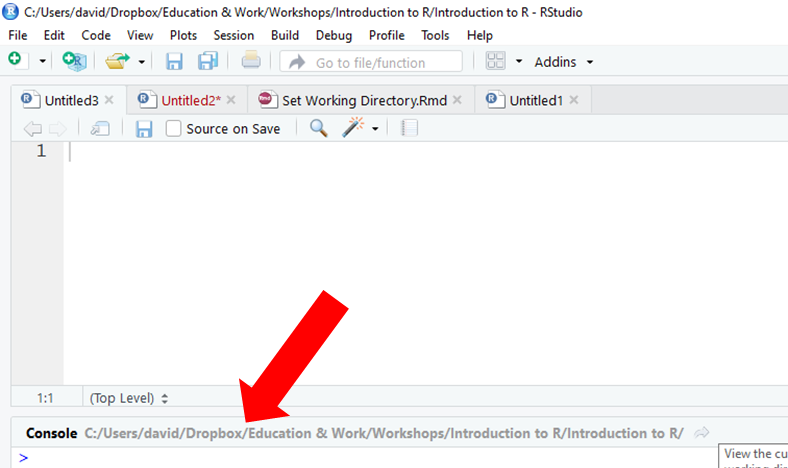
\includegraphics{ConsoleWD.png}
\caption{}
\end{figure}

\subsection{Setting a New Working
Directory}\label{setting-a-new-working-directory}

Let's assume that the current working directory is \emph{not} what we
want; meaning, we need to set a new or different working directory. If
you need to set a new working directory, you can use the \texttt{setwd}
function from base R. Within the parentheses, your only argument will be
the working directory in quotation marks. I recommend typing your
\texttt{setwd} function into an R Script (.R) file so that it can be
saved for future sessions. I also recommend using the \texttt{\#} to
annotate your script so that you can remind yourself (and others) what
you are doing.

When it comes to working directories, R likes the forward slash
(\texttt{/}) (as opposed to backslash). Remember, the working directory
is the location of the data files you wish to access and bring into the
R environment. You can access any folder you would like and set it as
your working directory.

\begin{Shaded}
\begin{Highlighting}[]
\CommentTok{# Set your working directory}
\KeywordTok{setwd}\NormalTok{(}\StringTok{"H:/RWorkshop"}\NormalTok{)}
\end{Highlighting}
\end{Shaded}

Alternatively, you may use the drop-down menus to select a working
directory folder. To do so, go to \emph{Session \textgreater{} Set
Working Directory \textgreater{} Choose Directory\ldots{}}, and select
the folder where your files live. Upon doing so, your working directory
will appear in the Console. You can copy and paste the working directory
into your \texttt{setwd} function.

\begin{figure}
\centering
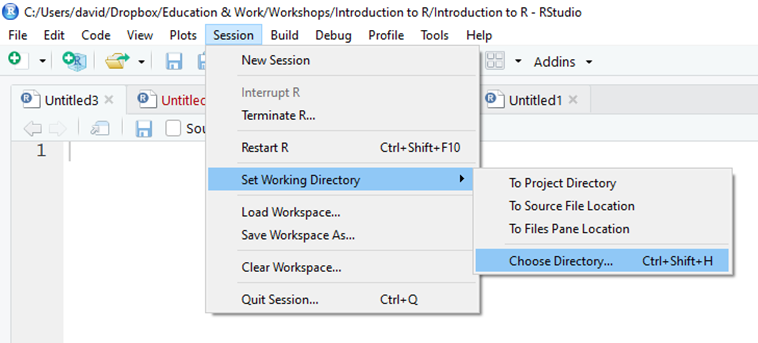
\includegraphics{Set Working Directory.png}
\caption{}
\end{figure}

Once you have set your working directory, you can verify that it was set
to the correct folder by (a) typing \texttt{getwd()} into your console
or (b) looking at the working directory listed next to the word
``Console'' in your Console window.

\hypertarget{createRscript}{\section{Creating \& Saving an R
Script}\label{createRscript}}

An \textbf{R Script} is a text editor file in which you can create,
edit, and save your R code for a particular task or project. An R Script
file has the .R file extension. It is advisable that you type code
directly into an R Script file if you wish to use the code again in the
future or if you wish to save the code for another session. In general,
try to avoid writing code directly into the Console using the command
line if you wish to later reproduce your work. An R Script also allows
you to make and save annotations (using the \texttt{\#} symbol) to
explain your code and decision making. Once you typed code (and
annotations) into an R Script, you can highlight all of it (or chunks of
it) and then click the Run button (or CTRL+Enter for Windows users or
Command+Enter for Mac users), which is located in the upper right hand
corner of the R Script editor window.

In essence, an R Script allows you to save your code and to tell a story
about what you have done. As much as you believe you'll never forget
what you were doing in a particular R session, you will likely forget
important details as time passes. Or, imagine a scenario in which
someone else inherits your data project; a well-written and -documented
R Script file will help them retrace your footsteps and onboard them
onto the project.

\subsubsection{Video Tutorial}\label{video-tutorial-2}

Link to Video Tutorial: \url{https://youtu.be/6_CFx5-KmMI}

\subsection{Creating a New R Script}\label{creating-a-new-r-script}

To create a new R Script in RStudio, in the drop-down menu, select
\emph{File \textgreater{} New File \textgreater{} R Script} (as shown
below).

\begin{figure}
\centering
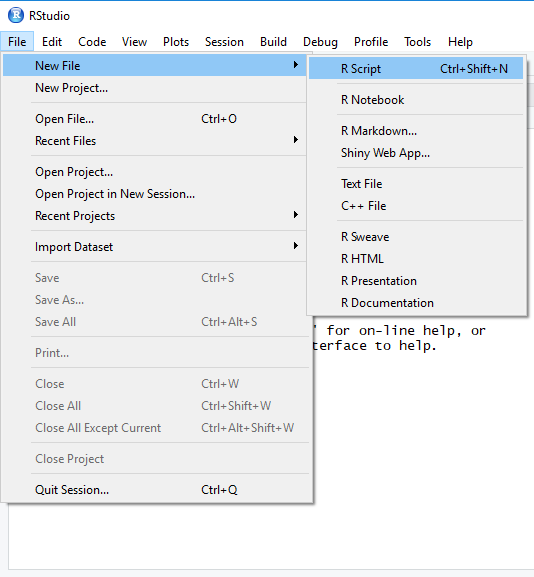
\includegraphics{New R Script.png}
\caption{}
\end{figure}

\subsection{Using an R Script}\label{using-an-r-script}

To use an R Script, simply type into the script interface. To illustrate
how to do this, let's type \texttt{\#\ Adding\ 2\ plus\ 3} on the first
line; note that I began the line with the \texttt{\#} symbol, which
tells R that any text written to the right is annotation and thus won't
be interpreted by R when you select it and click Run. On the next line,
let's type \texttt{2\ +\ 3}. Highlight both lines of script you typed
and click the Run button (or CTRL+Enter for Windows users or
Command+Enter for Mac users) (as shown below).

\begin{figure}
\centering
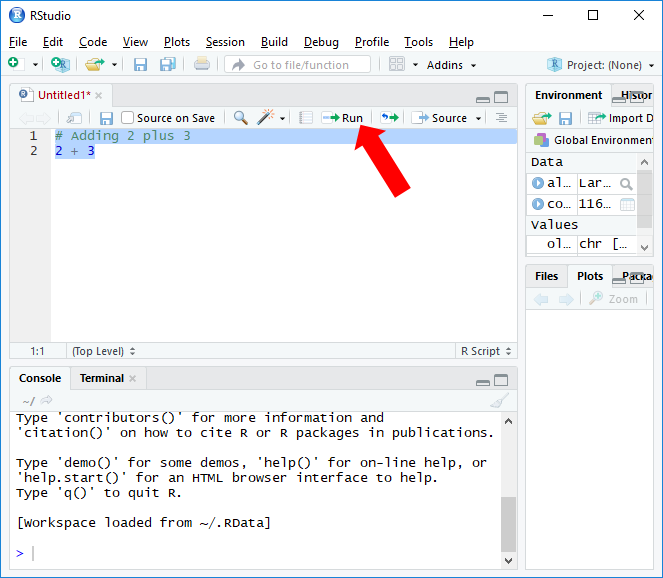
\includegraphics{Using an R Script.png}
\caption{}
\end{figure}

\begin{Shaded}
\begin{Highlighting}[]
\CommentTok{# Adding 2 plus 3}
\DecValTok{2} \OperatorTok{+}\StringTok{ }\DecValTok{3}
\end{Highlighting}
\end{Shaded}

\begin{verbatim}
## [1] 5
\end{verbatim}

Your Console window should show your output (as shown above).

\subsection{Saving an R Script}\label{saving-an-r-script}

Always remember to save your R Script, and do so frequently. To save an
R Script in RStudio, in the drop-down menu, select \emph{File
\textgreater{} Save As} (as shown below). After that, a window will
open, and you can save the R Script file in a location of your choosing
and with a name of your choosing.

\begin{figure}
\centering
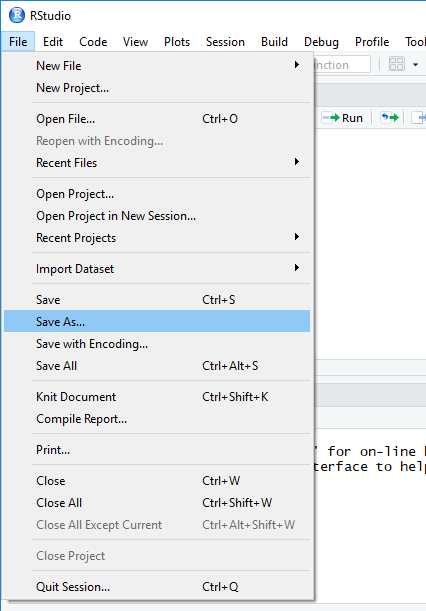
\includegraphics{Saving R Script.png}
\caption{}
\end{figure}

\subsection{Opening a Saved R Script}\label{opening-a-saved-r-script}

To open a saved R Script in RStudio, in the drop-down menu, select
\emph{File \textgreater{} Open File\ldots{}} (as shown below). After
that, a window will open, and you can select the R Script file to open.

\begin{figure}
\centering
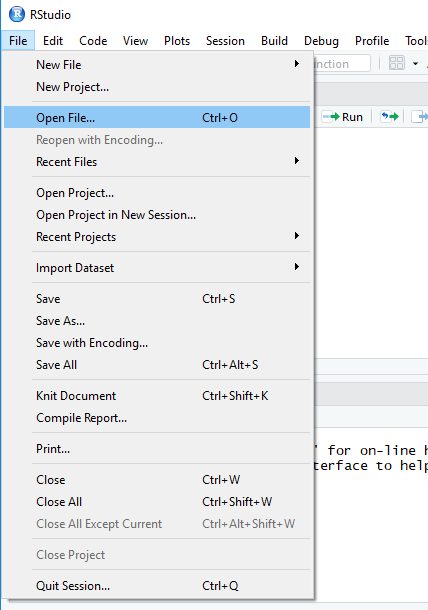
\includegraphics{Opening R Script.png}
\caption{}
\end{figure}

\section{Creating an RStudio Project}\label{creating-an-rstudio-project}

An \textbf{RStudio project} (or \textbf{R project}) file (.Rproj) is
specific to RStudio and allows one to cluster associated scripts and
data files into into a single workflow. For example, if you were
evaluating a new onboarding program for your company, you could create
an RStudio project with a common working directory that ties together
any data files and R scripts that are relevant for evaluating the
program. Creating an R project is not required for data management,
analysis, and visualization work in RStudio, but it can be helpful. For
more information on the value of RStudio projects, check out Wickham and
Grolemund's \citeyearpar{wickham2017} section on RStudio projects:
\url{https://r4ds.had.co.nz/workflow-projects.html\#rstudio-projects}.

\subsubsection{Video Tutorial}\label{video-tutorial-3}

Link to Video Tutorial: \url{https://youtu.be/WyrJmJWgPiU}

\subsection{Creating a New RStudio
Project}\label{creating-a-new-rstudio-project}

\textbf{First}, to create a new project in RStudio, in the drop-down
menu, select \emph{File \textgreater{} New Project\ldots{}}.

\begin{figure}
\centering
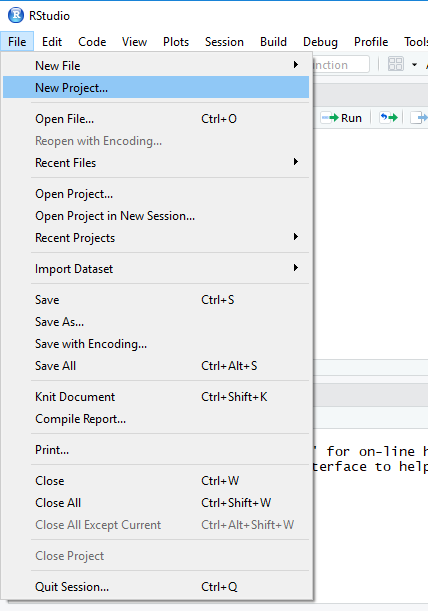
\includegraphics{Create R Project.png}
\caption{}
\end{figure}

\textbf{Second}, when the ``Create Project'' window pops up, select the
``New Directory'' option if you have not yet created a working directory
that can be used for your project (see Figure 2). {[}Alternatively,
select the ``Existing Directory'' option if already have a working
directory in place that can be used for your project.{]}

\begin{figure}
\centering
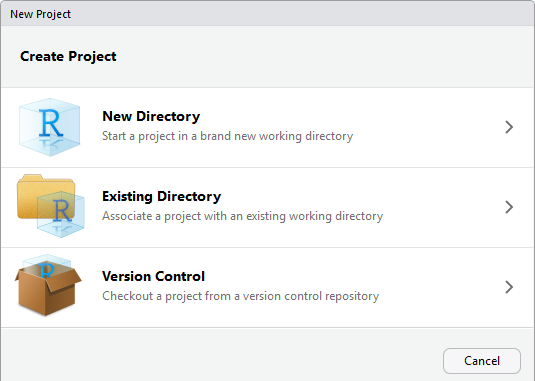
\includegraphics{Project Window.png}
\caption{}
\end{figure}

\textbf{Third}, in the ``Project Type'' window, select ``New Project''.

\begin{figure}
\centering
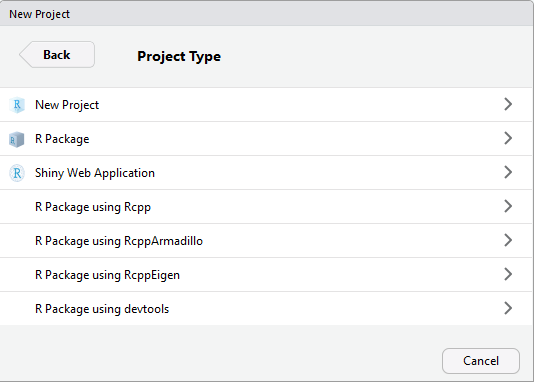
\includegraphics{Project Type.png}
\caption{}
\end{figure}

\textbf{Fourth}, in the ``Create New Project'' window, input what you
would like to name the new project (in the field under ``Directory
name'') and select the location of your working directory. Finally,
click the ``Create Project'' button.

\begin{figure}
\centering
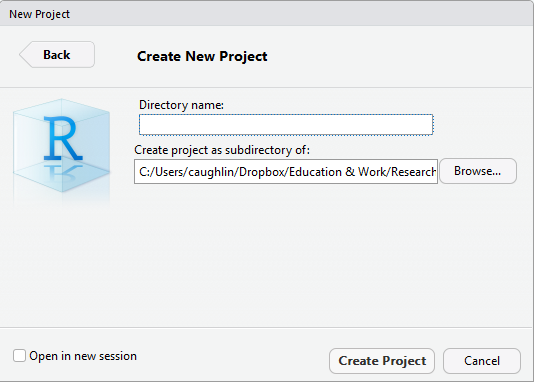
\includegraphics{Create New Project.png}
\caption{}
\end{figure}

\subsection{Opening an Existing RStudio
Project}\label{opening-an-existing-rstudio-project}

To open an existing RStudio project, in the drop-down menu, select
\emph{File \textgreater{} Open Project\ldots{}}.

\begin{figure}
\centering
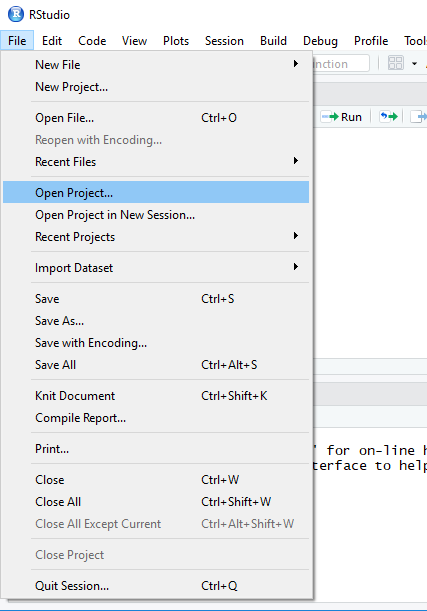
\includegraphics{Open Project.png}
\caption{}
\end{figure}

\section{Orientation to Written
Tutorials}\label{orientation-to-written-tutorials}

Throughout this book, I have included example R code, which I did so
using RMarkdown. This approach to demonstrating R tools and techniques
is common, and thus it's good to orient yourself to written tutorials in
this format. The following video provides an orientation to written R
tutorials.

\subsubsection{Video Tutorial}\label{video-tutorial-4}

Link to Video Tutorial: \url{https://youtu.be/1Wh6eUYAoZc}

\section{Summary}\label{summary}

In this chapter, you learned how to set a working directory, create an R
script, create an RStudio project, and orient yourself to written R
tutorials. First, setting the working directory is often an important
step when reading (importing) and writing (exporting objects) in R. You
can use the \texttt{getwd} function to check where your current working
directory is, whereas the \texttt{setwd} can be used to set a new
working directory. Second, writing and saving your R code in an R Script
file (.R) is an important step towards reproducible data management,
analysis, and visualization. Third, creating an RStudio project can
streamline data-analytic projects and provides some user-friendly
features. Finally, written R tutorials are common in both printed and
web-based formats, and thus it's worthwhile to familiarize yourself with
how to follow along with these types of tutorials.

\hypertarget{gentleintro}{\chapter{Basic Features and Operations of the
R Language}\label{gentleintro}}

In this chapter, you will learn about basic features of the R language
along with key bits of terminology. Think of this chapter as a ``gentle
introduction to R.''

\subsubsection{Video Tutorial}\label{video-tutorial}

Link to Video Tutorial: \url{https://youtu.be/yHbVbHEjhLQ}

\subsubsection{Functions \& Packages
Introduced}\label{functions-packages-introduced}

\begin{longtable}[]{@{}ll@{}}
\toprule
Function & Package\tabularnewline
\midrule
\endhead
\texttt{print} & base\tabularnewline
\texttt{class} & base\tabularnewline
\texttt{str} & base\tabularnewline
\texttt{install.packages} & base\tabularnewline
\texttt{library} & base\tabularnewline
\texttt{is.numeric} & base\tabularnewline
\texttt{is.integer} & base\tabularnewline
\texttt{is.character} & base\tabularnewline
\texttt{is.logical} & base\tabularnewline
\texttt{as.Date} & base\tabularnewline
\texttt{as.POSIXct} & base\tabularnewline
\texttt{c} & base\tabularnewline
\texttt{data.frame} & base\tabularnewline
\texttt{names} & base\tabularnewline
\bottomrule
\end{longtable}

\section{R as a Calculator}\label{r-as-a-calculator}

In its simplest form, R is a calculator. You can use R to carry out
basic arithmetic, algebra, and other mathematical operations. The
arithmetic operators in R are \texttt{+} (addition), \texttt{-}
(subtraction), \texttt{*} (multiplication), \texttt{/} (division),
\texttt{\^{}} (exponent), and \texttt{sqrt} (square root). Below, you
will find an example of these different arithmetic operators in action.
In this book, lines of output are preceded by double hashtags
(\texttt{\#\#}); however, in your own R Console, you will not see the
double hashtags before your output -- unless, that is, you use double
hashtags before your lines of script
\protect\hyperlink{annotate}{annotations}.

\begin{Shaded}
\begin{Highlighting}[]
\DecValTok{3} \OperatorTok{+}\StringTok{ }\DecValTok{2}
\end{Highlighting}
\end{Shaded}

\begin{verbatim}
## [1] 5
\end{verbatim}

\begin{Shaded}
\begin{Highlighting}[]
\DecValTok{3} \OperatorTok{-}\StringTok{ }\DecValTok{2}
\end{Highlighting}
\end{Shaded}

\begin{verbatim}
## [1] 1
\end{verbatim}

\begin{Shaded}
\begin{Highlighting}[]
\DecValTok{3} \OperatorTok{*}\StringTok{ }\DecValTok{2}
\end{Highlighting}
\end{Shaded}

\begin{verbatim}
## [1] 6
\end{verbatim}

\begin{Shaded}
\begin{Highlighting}[]
\DecValTok{3} \OperatorTok{/}\StringTok{ }\DecValTok{2}
\end{Highlighting}
\end{Shaded}

\begin{verbatim}
## [1] 1.5
\end{verbatim}

\begin{Shaded}
\begin{Highlighting}[]
\DecValTok{3} \OperatorTok{^}\StringTok{ }\DecValTok{2}
\end{Highlighting}
\end{Shaded}

\begin{verbatim}
## [1] 9
\end{verbatim}

\begin{Shaded}
\begin{Highlighting}[]
\KeywordTok{sqrt}\NormalTok{(}\DecValTok{3}\NormalTok{)}
\end{Highlighting}
\end{Shaded}

\begin{verbatim}
## [1] 1.732051
\end{verbatim}

Note how the six lines of output we generated (see above) appear in the
same order in your Console; relatedly, remember that in R (like many
other languages) the order of operations is important.

In R it doesn't matter whether there are spaces between the numeric
values and the arithmetic operators. As such, we can write our code as
follows and arrive at the same output.

\begin{Shaded}
\begin{Highlighting}[]
\DecValTok{3}\OperatorTok{+}\DecValTok{2}
\end{Highlighting}
\end{Shaded}

\begin{verbatim}
## [1] 5
\end{verbatim}

\begin{Shaded}
\begin{Highlighting}[]
\DecValTok{3}\OperatorTok{-}\DecValTok{2}
\end{Highlighting}
\end{Shaded}

\begin{verbatim}
## [1] 1
\end{verbatim}

\begin{Shaded}
\begin{Highlighting}[]
\DecValTok{3}\OperatorTok{*}\DecValTok{2}
\end{Highlighting}
\end{Shaded}

\begin{verbatim}
## [1] 6
\end{verbatim}

\begin{Shaded}
\begin{Highlighting}[]
\DecValTok{3}\OperatorTok{/}\DecValTok{2}
\end{Highlighting}
\end{Shaded}

\begin{verbatim}
## [1] 1.5
\end{verbatim}

\begin{Shaded}
\begin{Highlighting}[]
\DecValTok{3}\OperatorTok{^}\DecValTok{2}
\end{Highlighting}
\end{Shaded}

\begin{verbatim}
## [1] 9
\end{verbatim}

\begin{Shaded}
\begin{Highlighting}[]
\KeywordTok{sqrt}\NormalTok{(}\DecValTok{3}\NormalTok{)}
\end{Highlighting}
\end{Shaded}

\begin{verbatim}
## [1] 1.732051
\end{verbatim}

\section{Functions}\label{functions}

A \textbf{function} refers to an integrated set of instructions that can
be applied consistently. Some functions also accept arguments, where an
\textbf{argument} is used to further refine the instructions and
resulting operations of the function. In R we can use functions that
come standard from base R or functions that come from downloadable
packages. Let's take a look at the \texttt{print} function that comes
standard with base R, which means that we don't need a special package
to access the function. This won't be terribly exciting, but we can
enter \texttt{3} as an argument within the \texttt{print} function
parentheses; in general, arguments will appear within the inclusive
parentheses.

\begin{Shaded}
\begin{Highlighting}[]
\KeywordTok{print}\NormalTok{(}\DecValTok{3}\NormalTok{)}
\end{Highlighting}
\end{Shaded}

\begin{verbatim}
## [1] 3
\end{verbatim}

Note how the \texttt{print} function simply ``printed'' the numeric
value \texttt{3} that we entered.

We can also do the classic - yet super cliche - ``Hello world!'' example
to illustrate how R and the \texttt{print} function handle
text/character/string data; except, let's change it to
\texttt{"Hello\ HR\ Analytics!"}.

\begin{Shaded}
\begin{Highlighting}[]
\KeywordTok{print}\NormalTok{(}\StringTok{"Hello HR Analytics!"}\NormalTok{)}
\end{Highlighting}
\end{Shaded}

\begin{verbatim}
## [1] "Hello HR Analytics!"
\end{verbatim}

Note how we have to put text/character/string data in quotation marks.
We can use double (\texttt{"\ "}) or single quotes
(\texttt{\textquotesingle{}\ \textquotesingle{}}). Some people prefer
double quotes and some prefer single quotes. I happen to prefer double
quotes.

Now, let's play around with the \texttt{class} function. The
\texttt{class} function is used for determining the data type
represented by a datum or by multiple data that are contained in a
vector or variable. By entering \texttt{3} as an argument in the
\texttt{class} variable, we find that the data type is \texttt{numeric}.

\begin{Shaded}
\begin{Highlighting}[]
\KeywordTok{class}\NormalTok{(}\DecValTok{3}\NormalTok{)}
\end{Highlighting}
\end{Shaded}

\begin{verbatim}
## [1] "numeric"
\end{verbatim}

If you would like to learn more about a function and the types of
arguments that can be used within the function, you can access the help
feature in R to access documentation on the function. The easiest way to
do this is to enter \texttt{?} before the name of the function. Upon
doing so, a help window will open; if you're using RStudio, a specific
window pane dedicated to Help will open.

\begin{Shaded}
\begin{Highlighting}[]
\NormalTok{?class}
\end{Highlighting}
\end{Shaded}

\hypertarget{packages}{\section{Packages}\label{packages}}

A \textbf{package} is a collection of functions with a common theme or
that can be applied to address a similar set of problems. R packages go
through a rigorous and laborious development and vetting process before
being posted on the CRAN website (\url{https://cran.r-project.org/}).

There are two functions that are important when it comes to installing
and using packages. First, the \texttt{install.packages} function is
used to install a package. The name of the package you wish to install
should be surrounded with quotation marks (\texttt{"\ "} or
\texttt{\textquotesingle{}\ \textquotesingle{}}) and entered as an
argument in the function. For example, if we wish to install the
\texttt{lessR} package \citep{R-lessR2020}, we type
\texttt{install.packages("lessR")}, as shown below. Please note that the
names of packages (and functions, arguments, and objects) are case
sensitive in R.

\begin{Shaded}
\begin{Highlighting}[]
\KeywordTok{install.packages}\NormalTok{(}\StringTok{"lessR"}\NormalTok{)}
\end{Highlighting}
\end{Shaded}

Once you have installed a package, you use the \texttt{library} function
to ``check out'' the package from your ``library'' of functions. To use
the function, enter the exact name of the function \emph{without}
quotation marks.

\begin{Shaded}
\begin{Highlighting}[]
\KeywordTok{library}\NormalTok{(lessR)}
\end{Highlighting}
\end{Shaded}

\section{Variable Assignment}\label{variable-assignment}

\textbf{Variable assignment} is the process of assigning a value or
multiple values to a variable. There are two assignment operators that
can be used for variable assignment as well as for (re)naming objects
such as tables and data frames: \texttt{\textless{}-} and \texttt{=}.
Both work the same way. I prefer to use \texttt{\textless{}-}, but
others prefer \texttt{=}. In the example below, we assign the value
\texttt{3} to a variable (i.e., object) we are naming \texttt{x}.

\begin{Shaded}
\begin{Highlighting}[]
\NormalTok{x <-}\StringTok{ }\DecValTok{3}
\end{Highlighting}
\end{Shaded}

\begin{Shaded}
\begin{Highlighting}[]
\NormalTok{x =}\StringTok{ }\DecValTok{3}
\end{Highlighting}
\end{Shaded}

Both functions achieved the same end, and the function that was run most
recently overrides the previous attempt at assigning \texttt{3} to
\texttt{x}. Using the \texttt{print} function we check with this worked.

\begin{Shaded}
\begin{Highlighting}[]
\KeywordTok{print}\NormalTok{(x)}
\end{Highlighting}
\end{Shaded}

\begin{verbatim}
## [1] 3
\end{verbatim}

Or, instead of using the \texttt{print} function , we can simply run
\texttt{x} by itself.

\begin{Shaded}
\begin{Highlighting}[]
\NormalTok{x}
\end{Highlighting}
\end{Shaded}

\begin{verbatim}
## [1] 3
\end{verbatim}

\section{Types of Data}\label{types-of-data}

In general, there are four different types of data in R:
\texttt{numeric}, \texttt{character}, \texttt{Date}, and
\texttt{logical}.

\subsection{\texorpdfstring{\texttt{numeric}
Data}{numeric Data}}\label{numeric-data}

\texttt{numeric} data are numbers or numeric values. This data type is
ready-made for quantitative analysis. We can apply the
\texttt{is.numeric} function to determine whether a value or variable is
\texttt{numeric}; if the value or variable entered as an argument is
\texttt{numeric}, R will return \texttt{TRUE}, and if it is not
\texttt{numeric}, R will return \texttt{FALSE}. {[}Note that
\texttt{TRUE} and \texttt{FALSE} statements don't require quotation
marks like text/character/string data, as they are handled differently
in R.{]} Finally, let's see if that \texttt{"Hello\ data\ science!"}
phrase is numeric.

\begin{Shaded}
\begin{Highlighting}[]
\KeywordTok{is.numeric}\NormalTok{(}\DecValTok{3}\NormalTok{)}
\end{Highlighting}
\end{Shaded}

\begin{verbatim}
## [1] TRUE
\end{verbatim}

\begin{Shaded}
\begin{Highlighting}[]
\KeywordTok{is.numeric}\NormalTok{(}\OtherTok{TRUE}\NormalTok{)}
\end{Highlighting}
\end{Shaded}

\begin{verbatim}
## [1] FALSE
\end{verbatim}

\begin{Shaded}
\begin{Highlighting}[]
\KeywordTok{is.numeric}\NormalTok{(}\StringTok{"Hello data science!"}\NormalTok{)}
\end{Highlighting}
\end{Shaded}

\begin{verbatim}
## [1] FALSE
\end{verbatim}

An \texttt{integer} is a special type of \texttt{numeric} data. An
\texttt{integer} does not have any decimals, and thus is a whole number.
To specify that \texttt{numeric} data are of type \texttt{integer},
\texttt{L} must be appended to the value. For example, to specify that
\texttt{3} is an \texttt{integer}, it should be written as \texttt{3L}.
To verify that a value is in fact of type \texttt{integer}, we can apply
the \texttt{as.integer} function.

\begin{Shaded}
\begin{Highlighting}[]
\KeywordTok{is.integer}\NormalTok{(3L)}
\end{Highlighting}
\end{Shaded}

\begin{verbatim}
## [1] TRUE
\end{verbatim}

\begin{Shaded}
\begin{Highlighting}[]
\KeywordTok{is.integer}\NormalTok{(}\DecValTok{3}\NormalTok{)}
\end{Highlighting}
\end{Shaded}

\begin{verbatim}
## [1] FALSE
\end{verbatim}

Alternatively, we can use the \texttt{class} or \texttt{str} functions
to determine whether a value or variable is \texttt{integer} or
\texttt{numeric}. The function \texttt{str} is used to identify the
structure of an object (e.g., data frame, variable, value).

\begin{Shaded}
\begin{Highlighting}[]
\KeywordTok{class}\NormalTok{(3L)}
\end{Highlighting}
\end{Shaded}

\begin{verbatim}
## [1] "integer"
\end{verbatim}

\begin{Shaded}
\begin{Highlighting}[]
\KeywordTok{str}\NormalTok{(3L)}
\end{Highlighting}
\end{Shaded}

\begin{verbatim}
##  int 3
\end{verbatim}

\begin{Shaded}
\begin{Highlighting}[]
\KeywordTok{class}\NormalTok{(}\DecValTok{3}\NormalTok{)}
\end{Highlighting}
\end{Shaded}

\begin{verbatim}
## [1] "numeric"
\end{verbatim}

\begin{Shaded}
\begin{Highlighting}[]
\KeywordTok{str}\NormalTok{(}\DecValTok{3}\NormalTok{)}
\end{Highlighting}
\end{Shaded}

\begin{verbatim}
##  num 3
\end{verbatim}

Finally, if we assign a \texttt{numeric} or \texttt{integer} value to a
variable, the resulting variable will take on the \texttt{numeric} or
\texttt{integer} data type (respectively).

\begin{Shaded}
\begin{Highlighting}[]
\NormalTok{x <-}\StringTok{ }\DecValTok{3}
\KeywordTok{class}\NormalTok{(x)}
\end{Highlighting}
\end{Shaded}

\begin{verbatim}
## [1] "numeric"
\end{verbatim}

\begin{Shaded}
\begin{Highlighting}[]
\NormalTok{x <-}\StringTok{ }\NormalTok{3L}
\KeywordTok{class}\NormalTok{(x)}
\end{Highlighting}
\end{Shaded}

\begin{verbatim}
## [1] "integer"
\end{verbatim}

\subsection{\texorpdfstring{\texttt{character}
Data}{character Data}}\label{character-data}

Data of type \texttt{character} do not explicitly or innately have
quantitative properties. Sometimes this type of data is called
``string'' or ``text'' data. Data of type \texttt{factor} is similar to
\texttt{character} but handled differently by R; this distinction
becomes more important when working with vectors and analyses. That
said, many analysis functions automatically convert \texttt{character}
to \texttt{factor} for analyses, but when it comes to working with and
manipulating data frames, this \texttt{character} versus \texttt{factor}
distinction becomes more important. When data are of type
\texttt{character}, we place quotation marks (\texttt{"\ "} or
\texttt{\textquotesingle{}\ \textquotesingle{}}) around the text. For
example, if the \texttt{character} of interest is \texttt{old}, then we
place quotation marks around text like this \texttt{"old"}. Also note
that \texttt{character} data are case sensitive, which means that
\texttt{"old"} is not the same as \texttt{"Old"}. Using the function
\texttt{is.character}, we can determine whether data are in fact of type
\texttt{character}.

\begin{Shaded}
\begin{Highlighting}[]
\KeywordTok{is.character}\NormalTok{(}\StringTok{"old"}\NormalTok{)}
\end{Highlighting}
\end{Shaded}

\begin{verbatim}
## [1] TRUE
\end{verbatim}

Note how omitting the \texttt{"\ "} results in an error message.

\begin{Shaded}
\begin{Highlighting}[]
\KeywordTok{is.character}\NormalTok{(old)}
\end{Highlighting}
\end{Shaded}

\begin{verbatim}
## Error in eval(expr, envir, enclos): object 'old' not found
\end{verbatim}

Finally, if we assign a \texttt{numeric} or \texttt{integer} value to a
variable, the resulting variable will take on the \texttt{numeric} or
\texttt{integer} data types.

\begin{Shaded}
\begin{Highlighting}[]
\NormalTok{y <-}\StringTok{ "old"}
\KeywordTok{class}\NormalTok{(y)}
\end{Highlighting}
\end{Shaded}

\begin{verbatim}
## [1] "character"
\end{verbatim}

\subsection{\texorpdfstring{\texttt{Date}
Data}{Date Data}}\label{date-data}

When working with dates in R, there are two different types:
\texttt{Date} and \texttt{POSIXct}. \texttt{Date} captures just the
date, whereas \texttt{POSIXct} captures the date and time. Behind the
scenes, R treats \texttt{Date} numerically as the number of days since
January 1, 1970, and \texttt{POSIXct} as the number of seconds since
January 1, 1970. To specify a value as a date, we can use the
\texttt{as.Date} function.

\begin{Shaded}
\begin{Highlighting}[]
\NormalTok{z <-}\StringTok{ }\KeywordTok{as.Date}\NormalTok{(}\StringTok{"1970-03-01"}\NormalTok{)}
\KeywordTok{class}\NormalTok{(z)}
\end{Highlighting}
\end{Shaded}

\begin{verbatim}
## [1] "Date"
\end{verbatim}

If we convert a variable of type \texttt{Date} to \texttt{numeric} using
the \texttt{as.numeric} function, the result is the number of days since
January 1, 1970.

\begin{Shaded}
\begin{Highlighting}[]
\NormalTok{z <-}\StringTok{ }\KeywordTok{as.Date}\NormalTok{(}\StringTok{"1970-03-01"}\NormalTok{)}
\KeywordTok{as.numeric}\NormalTok{(z)}
\end{Highlighting}
\end{Shaded}

\begin{verbatim}
## [1] 59
\end{verbatim}

Now we can use the \texttt{as.POSIXct} function to specify a value as a
date and time. Note the very specific format in which the data and time
are to be written.

\begin{Shaded}
\begin{Highlighting}[]
\NormalTok{z <-}\StringTok{ }\KeywordTok{as.POSIXct}\NormalTok{(}\StringTok{"1970-03-01 13:10"}\NormalTok{)}
\KeywordTok{class}\NormalTok{(z)}
\end{Highlighting}
\end{Shaded}

\begin{verbatim}
## [1] "POSIXct" "POSIXt"
\end{verbatim}

If we convert a variable of type \texttt{POSIXct} to \texttt{numeric}
using the \texttt{as.numeric} function, the result is the number of
seconds since January 1, 1970.

\begin{Shaded}
\begin{Highlighting}[]
\NormalTok{z <-}\StringTok{ }\KeywordTok{as.POSIXct}\NormalTok{(}\StringTok{"1970-03-01 13:10"}\NormalTok{)}
\KeywordTok{as.numeric}\NormalTok{(z)}
\end{Highlighting}
\end{Shaded}

\begin{verbatim}
## [1] 5173800
\end{verbatim}

\subsection{\texorpdfstring{\texttt{logical}
Data}{logical Data}}\label{logical-data}

Data that are of type \texttt{logical} can take on values of either
\texttt{TRUE} or \texttt{FALSE}, which correspond to the integers
\texttt{1} and \texttt{0}, respectively. As mentioned above, although
\texttt{TRUE} and \texttt{FALSE} appear to be \texttt{character} or
\texttt{factor} data, they are actually \texttt{logical} data, which
means they do not require quotation marks (\texttt{"\ "} or
\texttt{\textquotesingle{}\ \textquotesingle{}}).

\begin{Shaded}
\begin{Highlighting}[]
\NormalTok{w <-}\StringTok{ }\OtherTok{FALSE}
\KeywordTok{class}\NormalTok{(w)}
\end{Highlighting}
\end{Shaded}

\begin{verbatim}
## [1] "logical"
\end{verbatim}

\begin{Shaded}
\begin{Highlighting}[]
\KeywordTok{is.logical}\NormalTok{(w)}
\end{Highlighting}
\end{Shaded}

\begin{verbatim}
## [1] TRUE
\end{verbatim}

\section{Vectors}\label{vectors}

A \textbf{vector} is a group of data elements in a particular order that
are all the same data type. To create a vector, we can use the
\texttt{c} function, which stands for ``combine.'' Within the \texttt{c}
function parentheses, we can list the data elements and separate them by
commas, as commas separate arguments within a function's parentheses. We
can also assign a vector to a variable using either the
\texttt{\textless{}-} or \texttt{=} operator. We can create vectors for
all of the data types: \texttt{numeric}, \texttt{character},
\texttt{Date}, and \texttt{logical}.

As an example, let's create a vector of \texttt{numeric} values, and
let's call it \texttt{a}.

\begin{Shaded}
\begin{Highlighting}[]
\NormalTok{a <-}\StringTok{ }\KeywordTok{c}\NormalTok{(}\DecValTok{1}\NormalTok{, }\DecValTok{4}\NormalTok{, }\DecValTok{7}\NormalTok{, }\DecValTok{11}\NormalTok{, }\DecValTok{19}\NormalTok{)}
\end{Highlighting}
\end{Shaded}

Using the \texttt{class} and \texttt{print} functions, we can determine
the class of our new \texttt{a} object and print its values,
respectively.

\begin{Shaded}
\begin{Highlighting}[]
\KeywordTok{class}\NormalTok{(a)}
\end{Highlighting}
\end{Shaded}

\begin{verbatim}
## [1] "numeric"
\end{verbatim}

\begin{Shaded}
\begin{Highlighting}[]
\KeywordTok{print}\NormalTok{(a)}
\end{Highlighting}
\end{Shaded}

\begin{verbatim}
## [1]  1  4  7 11 19
\end{verbatim}

Let's repeat this process by creating vectors containing
\texttt{integer}, \texttt{character}, \texttt{Date}, and
\texttt{logical} values.

\begin{Shaded}
\begin{Highlighting}[]
\NormalTok{b <-}\StringTok{ }\KeywordTok{c}\NormalTok{(3L, 10L, 2L, 5L, 5L)}
\KeywordTok{class}\NormalTok{(b)}
\end{Highlighting}
\end{Shaded}

\begin{verbatim}
## [1] "integer"
\end{verbatim}

\begin{Shaded}
\begin{Highlighting}[]
\KeywordTok{print}\NormalTok{(b)}
\end{Highlighting}
\end{Shaded}

\begin{verbatim}
## [1]  3 10  2  5  5
\end{verbatim}

\begin{Shaded}
\begin{Highlighting}[]
\NormalTok{c <-}\StringTok{ }\KeywordTok{c}\NormalTok{(}\StringTok{"old"}\NormalTok{, }\StringTok{"young"}\NormalTok{, }\StringTok{"young"}\NormalTok{, }\StringTok{"old"}\NormalTok{, }\StringTok{"young"}\NormalTok{)}
\KeywordTok{class}\NormalTok{(c)}
\end{Highlighting}
\end{Shaded}

\begin{verbatim}
## [1] "character"
\end{verbatim}

\begin{Shaded}
\begin{Highlighting}[]
\KeywordTok{print}\NormalTok{(c)}
\end{Highlighting}
\end{Shaded}

\begin{verbatim}
## [1] "old"   "young" "young" "old"   "young"
\end{verbatim}

\begin{Shaded}
\begin{Highlighting}[]
\NormalTok{d <-}\StringTok{ }\KeywordTok{as.Date}\NormalTok{(}\KeywordTok{c}\NormalTok{(}\StringTok{"2018-06-01"}\NormalTok{, }\StringTok{"2018-06-01"}\NormalTok{, }\StringTok{"2018-10-31"}\NormalTok{, }\StringTok{"2018-01-01"}\NormalTok{, }\StringTok{"2018-06-01"}\NormalTok{))}
\KeywordTok{class}\NormalTok{(d)}
\end{Highlighting}
\end{Shaded}

\begin{verbatim}
## [1] "Date"
\end{verbatim}

\begin{Shaded}
\begin{Highlighting}[]
\KeywordTok{print}\NormalTok{(d)}
\end{Highlighting}
\end{Shaded}

\begin{verbatim}
## [1] "2018-06-01" "2018-06-01" "2018-10-31" "2018-01-01" "2018-06-01"
\end{verbatim}

\begin{Shaded}
\begin{Highlighting}[]
\NormalTok{e <-}\StringTok{ }\KeywordTok{c}\NormalTok{(}\OtherTok{TRUE}\NormalTok{, }\OtherTok{TRUE}\NormalTok{, }\OtherTok{TRUE}\NormalTok{, }\OtherTok{FALSE}\NormalTok{, }\OtherTok{FALSE}\NormalTok{)}
\KeywordTok{class}\NormalTok{(e)}
\end{Highlighting}
\end{Shaded}

\begin{verbatim}
## [1] "logical"
\end{verbatim}

\begin{Shaded}
\begin{Highlighting}[]
\KeywordTok{print}\NormalTok{(e)}
\end{Highlighting}
\end{Shaded}

\begin{verbatim}
## [1]  TRUE  TRUE  TRUE FALSE FALSE
\end{verbatim}

We can also perform mathematical operations on vectors. For instance, we
can multiply vector \texttt{a} (which we created above) by a numeric
value, and as a result each vector value will be multiplied by that
value. This is an important type of operation to remember when it comes
time to transform a variable.

\begin{Shaded}
\begin{Highlighting}[]
\NormalTok{a }\OperatorTok{*}\StringTok{ }\DecValTok{11}
\end{Highlighting}
\end{Shaded}

\begin{verbatim}
## [1]  11  44  77 121 209
\end{verbatim}

Note that performing mathematical operations on a vector does not
automatically change the properties of the vector itself. If you inspect
the \texttt{a} vector, you will see that the original data (e.g.,
\texttt{1,\ 4,\ 7,\ 11,\ 19}) remain.

\begin{Shaded}
\begin{Highlighting}[]
\KeywordTok{print}\NormalTok{(a)}
\end{Highlighting}
\end{Shaded}

\begin{verbatim}
## [1]  1  4  7 11 19
\end{verbatim}

If we want to overwrite a vector with new values based on our
operations, we can use \texttt{\textless{}-} or \texttt{=} to name the
new vector (which, if named the same thing as the old vector, will
override the old vector) and, ultimately, to create a vector with the
operations applied to the original values.

\begin{Shaded}
\begin{Highlighting}[]
\NormalTok{a <-}\StringTok{ }\NormalTok{a }\OperatorTok{*}\StringTok{ }\DecValTok{11}
\KeywordTok{print}\NormalTok{(a)}
\end{Highlighting}
\end{Shaded}

\begin{verbatim}
## [1]  11  44  77 121 209
\end{verbatim}

To revert back to the original vector values for object \texttt{a}, we
can simply specify the original values using the \texttt{c} function
once more.

\begin{Shaded}
\begin{Highlighting}[]
\NormalTok{a <-}\StringTok{ }\KeywordTok{c}\NormalTok{(}\DecValTok{1}\NormalTok{, }\DecValTok{4}\NormalTok{, }\DecValTok{7}\NormalTok{, }\DecValTok{11}\NormalTok{, }\DecValTok{19}\NormalTok{)}
\end{Highlighting}
\end{Shaded}

Let's now apply subtraction, addition, and division operators to the
vector. Note that R adheres to the standard mathematical orders of
operation.

\begin{Shaded}
\begin{Highlighting}[]
\NormalTok{(}\DecValTok{3} \OperatorTok{+}\StringTok{ }\NormalTok{a) }\OperatorTok{/}\StringTok{ }\DecValTok{2} \OperatorTok{-}\StringTok{ }\DecValTok{1}
\end{Highlighting}
\end{Shaded}

\begin{verbatim}
## [1]  1.0  2.5  4.0  6.0 10.0
\end{verbatim}

We can also perform mathematical operations on vectors of the same
length (i.e., with the same number of data elements). In order, the
mathematical operator will be applied to each pair of vector values from
the respective vectors. Let's begin by creating a new vector called
\texttt{f}.

\begin{Shaded}
\begin{Highlighting}[]
\NormalTok{f <-}\StringTok{ }\KeywordTok{c}\NormalTok{(}\DecValTok{3}\NormalTok{, }\DecValTok{1}\NormalTok{, }\DecValTok{3}\NormalTok{, }\DecValTok{5}\NormalTok{, }\DecValTok{3}\NormalTok{)}
\end{Highlighting}
\end{Shaded}

Both \texttt{a} and \texttt{f} are the same length, which means we can
multiply, add, divide, subtract, and exponentiate

\begin{Shaded}
\begin{Highlighting}[]
\NormalTok{a }\OperatorTok{*}\StringTok{ }\NormalTok{f}
\end{Highlighting}
\end{Shaded}

\begin{verbatim}
## [1]  3  4 21 55 57
\end{verbatim}

\begin{Shaded}
\begin{Highlighting}[]
\NormalTok{a }\OperatorTok{+}\StringTok{ }\NormalTok{f}
\end{Highlighting}
\end{Shaded}

\begin{verbatim}
## [1]  4  5 10 16 22
\end{verbatim}

\begin{Shaded}
\begin{Highlighting}[]
\NormalTok{a }\OperatorTok{/}\StringTok{ }\NormalTok{f}
\end{Highlighting}
\end{Shaded}

\begin{verbatim}
## [1] 0.3333333 4.0000000 2.3333333 2.2000000 6.3333333
\end{verbatim}

\begin{Shaded}
\begin{Highlighting}[]
\NormalTok{a }\OperatorTok{-}\StringTok{ }\NormalTok{f}
\end{Highlighting}
\end{Shaded}

\begin{verbatim}
## [1] -2  3  4  6 16
\end{verbatim}

\begin{Shaded}
\begin{Highlighting}[]
\NormalTok{a }\OperatorTok{^}\StringTok{ }\NormalTok{f}
\end{Highlighting}
\end{Shaded}

\begin{verbatim}
## [1]      1      4    343 161051   6859
\end{verbatim}

\section{Lists}\label{lists}

If we wish to combine data elements into a single list that with
different data types, we can use the \texttt{list} function. The
\texttt{list} function orders each data element and retains its value.

\begin{Shaded}
\begin{Highlighting}[]
\NormalTok{g <-}\StringTok{ }\KeywordTok{list}\NormalTok{(}\DecValTok{1}\NormalTok{, }\StringTok{"dog"}\NormalTok{, }\OtherTok{TRUE}\NormalTok{, }\StringTok{"2018-05-30"}\NormalTok{)}
\KeywordTok{print}\NormalTok{(g)}
\end{Highlighting}
\end{Shaded}

\begin{verbatim}
## [[1]]
## [1] 1
## 
## [[2]]
## [1] "dog"
## 
## [[3]]
## [1] TRUE
## 
## [[4]]
## [1] "2018-05-30"
\end{verbatim}

\begin{Shaded}
\begin{Highlighting}[]
\KeywordTok{class}\NormalTok{(g)}
\end{Highlighting}
\end{Shaded}

\begin{verbatim}
## [1] "list"
\end{verbatim}

\section{Data Frames}\label{data-frames}

A \textbf{data frame} is a specific type of table in which columns
represent variables (i.e., fields) and rows represent cases (i.e.,
observations). We can create a simple data frame object by combining
vectors of the same length. Let's begin by creating six vector objects,
which we will label \texttt{a} through \texttt{f}.

\begin{Shaded}
\begin{Highlighting}[]
\NormalTok{a <-}\StringTok{ }\KeywordTok{c}\NormalTok{(}\DecValTok{1}\NormalTok{, }\DecValTok{4}\NormalTok{, }\DecValTok{7}\NormalTok{, }\DecValTok{11}\NormalTok{, }\DecValTok{19}\NormalTok{) }
\NormalTok{b <-}\StringTok{ }\KeywordTok{c}\NormalTok{(3L, 10L, 2L, 5L, 5L) }
\NormalTok{c <-}\StringTok{ }\KeywordTok{c}\NormalTok{(}\StringTok{"old"}\NormalTok{, }\StringTok{"young"}\NormalTok{, }\StringTok{"young"}\NormalTok{, }\StringTok{"old"}\NormalTok{, }\StringTok{"young"}\NormalTok{) }
\NormalTok{d <-}\StringTok{ }\KeywordTok{as.Date}\NormalTok{(}\KeywordTok{c}\NormalTok{(}\StringTok{"2018-06-01"}\NormalTok{, }\StringTok{"2018-06-01"}\NormalTok{, }\StringTok{"2018-10-31"}\NormalTok{, }\StringTok{"2018-01-01"}\NormalTok{, }\StringTok{"2018-06-01"}\NormalTok{)) }
\NormalTok{e <-}\StringTok{ }\KeywordTok{c}\NormalTok{(}\OtherTok{TRUE}\NormalTok{, }\OtherTok{TRUE}\NormalTok{, }\OtherTok{TRUE}\NormalTok{, }\OtherTok{FALSE}\NormalTok{, }\OtherTok{FALSE}\NormalTok{)}
\NormalTok{f <-}\StringTok{ }\KeywordTok{c}\NormalTok{(}\DecValTok{3}\NormalTok{, }\DecValTok{1}\NormalTok{, }\DecValTok{3}\NormalTok{, }\DecValTok{5}\NormalTok{, }\DecValTok{3}\NormalTok{)}
\end{Highlighting}
\end{Shaded}

Using the \texttt{data.frame} function from base R we can combine the
six vectors to create a data frame object. All we need to do is enter
the names of the six vectors as separate arguments in the function
parentheses. Just as we did with the vectors, we can name the data frame
object using the \texttt{\textless{}-} operator (or \texttt{=}
operator). Let's name this data frame object \texttt{r}.

\begin{Shaded}
\begin{Highlighting}[]
\NormalTok{r <-}\StringTok{ }\KeywordTok{data.frame}\NormalTok{(a, b, c, d, e, f)}
\end{Highlighting}
\end{Shaded}

Using the \texttt{print} function, we can view the contents of our new
data frame object called \texttt{r}.

\begin{Shaded}
\begin{Highlighting}[]
\KeywordTok{print}\NormalTok{(r)}
\end{Highlighting}
\end{Shaded}

\begin{verbatim}
##    a  b     c          d     e f
## 1  1  3   old 2018-06-01  TRUE 3
## 2  4 10 young 2018-06-01  TRUE 1
## 3  7  2 young 2018-10-31  TRUE 3
## 4 11  5   old 2018-01-01 FALSE 5
## 5 19  5 young 2018-06-01 FALSE 3
\end{verbatim}

We can also rename the columns (i.e., variables) of the data frame
object by using the \texttt{names} function from base R along with the
\texttt{c} function from base R.

\begin{Shaded}
\begin{Highlighting}[]
\KeywordTok{names}\NormalTok{(r) <-}\StringTok{ }\KeywordTok{c}\NormalTok{(}\StringTok{"TenureSup"}\NormalTok{, }\StringTok{"TenureOrg"}\NormalTok{, }\StringTok{"Age"}\NormalTok{, }\StringTok{"HireDate"}\NormalTok{, }\StringTok{"FTE"}\NormalTok{, }\StringTok{"NumEmp"}\NormalTok{)}
\end{Highlighting}
\end{Shaded}

To view the changes to our data frame object, use the \texttt{print}
function once more.

\begin{Shaded}
\begin{Highlighting}[]
\KeywordTok{print}\NormalTok{(r)}
\end{Highlighting}
\end{Shaded}

\begin{verbatim}
##   TenureSup TenureOrg   Age   HireDate   FTE NumEmp
## 1         1         3   old 2018-06-01  TRUE      3
## 2         4        10 young 2018-06-01  TRUE      1
## 3         7         2 young 2018-10-31  TRUE      3
## 4        11         5   old 2018-01-01 FALSE      5
## 5        19         5 young 2018-06-01 FALSE      3
\end{verbatim}

Finally, we can use the \texttt{class} function to verify that the
object is in fact a data frame.

\begin{Shaded}
\begin{Highlighting}[]
\KeywordTok{class}\NormalTok{(r)}
\end{Highlighting}
\end{Shaded}

\begin{verbatim}
## [1] "data.frame"
\end{verbatim}

\hypertarget{annotate}{\section{Annotations}\label{annotate}}

Part of the value of using a code/script-based program like R is that
you can leave notes and explain your decisions and operations. When
preceding text, the \texttt{\#} symbol indicates that all text that
follows on that line is a comment or annotation; as a result, R knows
not to interpret or analyze the text that follows. To illustrate
annotations, let's repeat the steps from the previous section; however,
this time, let's include annotations.

\begin{Shaded}
\begin{Highlighting}[]
\CommentTok{# Create six vectors }
\NormalTok{a <-}\StringTok{ }\KeywordTok{c}\NormalTok{(}\DecValTok{1}\NormalTok{, }\DecValTok{4}\NormalTok{, }\DecValTok{7}\NormalTok{, }\DecValTok{11}\NormalTok{, }\DecValTok{19}\NormalTok{) }\CommentTok{# Vector a}
\NormalTok{b <-}\StringTok{ }\KeywordTok{c}\NormalTok{(3L, 10L, 2L, 5L, 5L) }\CommentTok{# Vector b}
\NormalTok{c <-}\StringTok{ }\KeywordTok{c}\NormalTok{(}\StringTok{"old"}\NormalTok{, }\StringTok{"young"}\NormalTok{, }\StringTok{"young"}\NormalTok{, }\StringTok{"old"}\NormalTok{, }\StringTok{"young"}\NormalTok{) }\CommentTok{# Vector c}
\NormalTok{d <-}\StringTok{ }\KeywordTok{as.Date}\NormalTok{(}\KeywordTok{c}\NormalTok{(}\StringTok{"2018-06-01"}\NormalTok{, }\StringTok{"2018-06-01"}\NormalTok{, }\StringTok{"2018-10-31"}\NormalTok{, }\StringTok{"2018-01-01"}\NormalTok{, }\StringTok{"2018-06-01"}\NormalTok{)) }\CommentTok{# Vector d}
\NormalTok{e <-}\StringTok{ }\KeywordTok{c}\NormalTok{(}\OtherTok{TRUE}\NormalTok{, }\OtherTok{TRUE}\NormalTok{, }\OtherTok{TRUE}\NormalTok{, }\OtherTok{FALSE}\NormalTok{, }\OtherTok{FALSE}\NormalTok{) }\CommentTok{# Vector e}
\NormalTok{f <-}\StringTok{ }\KeywordTok{c}\NormalTok{(}\DecValTok{3}\NormalTok{, }\DecValTok{1}\NormalTok{, }\DecValTok{3}\NormalTok{, }\DecValTok{5}\NormalTok{, }\DecValTok{3}\NormalTok{) }\CommentTok{# Vector f}

\CommentTok{# Combine vectors into data frame}
\NormalTok{r <-}\StringTok{ }\KeywordTok{data.frame}\NormalTok{(a, b, c, d, e, f)}

\CommentTok{# Print data frame}
\KeywordTok{print}\NormalTok{(r)}
\end{Highlighting}
\end{Shaded}

\begin{verbatim}
##    a  b     c          d     e f
## 1  1  3   old 2018-06-01  TRUE 3
## 2  4 10 young 2018-06-01  TRUE 1
## 3  7  2 young 2018-10-31  TRUE 3
## 4 11  5   old 2018-01-01 FALSE 5
## 5 19  5 young 2018-06-01 FALSE 3
\end{verbatim}

\begin{Shaded}
\begin{Highlighting}[]
\CommentTok{# Rename columns in data frame}
\KeywordTok{names}\NormalTok{(r) <-}\StringTok{ }\KeywordTok{c}\NormalTok{(}\StringTok{"TenureSup"}\NormalTok{, }\StringTok{"TenureOrg"}\NormalTok{, }\StringTok{"Age"}\NormalTok{, }\StringTok{"HireDate"}\NormalTok{, }\StringTok{"FTE"}\NormalTok{, }\StringTok{"NumEmp"}\NormalTok{)}

\CommentTok{# Print data frame}
\KeywordTok{print}\NormalTok{(r)}
\end{Highlighting}
\end{Shaded}

\begin{verbatim}
##   TenureSup TenureOrg   Age   HireDate   FTE NumEmp
## 1         1         3   old 2018-06-01  TRUE      3
## 2         4        10 young 2018-06-01  TRUE      1
## 3         7         2 young 2018-10-31  TRUE      3
## 4        11         5   old 2018-01-01 FALSE      5
## 5        19         5 young 2018-06-01 FALSE      3
\end{verbatim}

\begin{Shaded}
\begin{Highlighting}[]
\CommentTok{# Determine class of object}
\KeywordTok{class}\NormalTok{(r)}
\end{Highlighting}
\end{Shaded}

\begin{verbatim}
## [1] "data.frame"
\end{verbatim}

Can you start to envision how annotated code might help to tell a story
about data-related decision-making processes?

\section{Summary}\label{summary}

This chapter provided you with a gentle introduction to R. This chapter
is by no means comprehensive, but hopefully it provided you with an
understanding of the basic operations and building blocks of R.

\part{Data Acquisition}\label{part-data-acquisition}

\hypertarget{read}{\chapter{Reading Data into R}\label{read}}

\textbf{Reading data} refers to the process of importing data from a
working directory or website into the R environment. When we read a data
file into R, we often read it in as a \textbf{data frame (df)}, where a
data frame is a tabular display with columns representing variables and
rows representing cases. Many different data file formats can be read
into R as data frames, such as .csv, .xls/x, .txt, .sas7bdat (SAS), and
.sav (SPSS). Finally, as you will learn in this tutorial, different
functions can be used to read data into R.

\subsubsection{Video Tutorial}\label{video-tutorial}

Link to Video Tutorial: \url{https://youtu.be/smWjqhaxHY8}

\subsubsection{Functions \& Packages
Introduced}\label{functions-packages-introduced}

\begin{longtable}[]{@{}ll@{}}
\toprule
Function & Package\tabularnewline
\midrule
\endhead
\texttt{read.csv} & base\tabularnewline
\texttt{read\_csv} & \texttt{readr}\tabularnewline
\texttt{Read} & \texttt{lessR}\tabularnewline
\texttt{excel\_sheets} & \texttt{readxl}\tabularnewline
\texttt{read\_excel} & \texttt{readxl}\tabularnewline
\texttt{View} & base\tabularnewline
\texttt{print} & base\tabularnewline
\texttt{head} & base\tabularnewline
\texttt{tail} & base\tabularnewline
\texttt{names} & base\tabularnewline
\texttt{colnames} & base\tabularnewline
\texttt{install.packages} & base\tabularnewline
\texttt{library} & base\tabularnewline
\texttt{list.files} & base\tabularnewline
\bottomrule
\end{longtable}

\subsubsection{Initial Steps}\label{initial-steps}

Please note, that any function that appears in the \emph{Initial Steps}
section has been covered in a previous chapter. If you need a refresher,
please view the relevant chapter. In addition, a previous chapter may
show you how to perform the same action using different functions or
packages.

To get started, please save the following data files into a folder on
your computer that you will set as your working directory:
\textbf{``PersData.csv''} and \textbf{``PersData\_Excel.xlsx''}. As a
reminder, you can access all of the data files referenced in this book
by downloading them as a compressed (zipped) folder from the my GitHub
site: \url{https://github.com/davidcaughlin/R-Tutorial-Data-Files}; once
you've followed the link to GitHub, just click ``Code'' (or
``Download'') followed by ``Download ZIP'', which will download all of
the data files referenced in this book. For the sake of parsimony, I
recommend downloading all of the data files into the same folder on your
computer, which will allow you to set that same folder as your working
directory for each of the chapters in this book.

Next, set your working directory by using the \texttt{setwd} function
(see below) or by doing it using drop-down menus. Your working directory
folder will likely be different than the one shown below;
``H:/RWorkshop'' just happens to be the name of the folder that I save
my data files to and that I set as my working directory. You can
manually set your working directory folder in your drop-down menus by
going to \emph{Session \textgreater{} Set Working Directory
\textgreater{} Choose Directory\ldots{}}. If you need a refresher on how
to set a working directory, please refer to
\protect\hyperlink{setwd}{Setting a Working Directory}.

\begin{Shaded}
\begin{Highlighting}[]
\CommentTok{# Set your working directory to the folder containing your data file}
\KeywordTok{setwd}\NormalTok{(}\StringTok{"H:/RWorkshop"}\NormalTok{)}
\end{Highlighting}
\end{Shaded}

Finally, I highly recommend that you create a new R Script file (.R),
which will allow you to edit and save your script and annotations. To
learn more, please refer to \protect\hyperlink{createRscript}{Creating
\& Saving an R Script}.

\section{Read Data}\label{read-data}

One of the easiest data file formats to work with when reading data into
R is the .csv (comma-separated values) format. The .csv (comma-separated
values) format is commonly used among R users, and such files can be
created in Microsoft Excel and Google Sheets (as well as other
programs). For example, many survey, data analysis, and data-acquisition
platforms allow data to be exported to .csv files. When getting started
in R, the way in which the .csv file is formatted can make your life
easier. Specifically, the most straightforward .csv file format to read
in is one in which the first row contains the name of each variable in
each column, and in which the second row contains the first row of
observed values (i.e., data) for the cases (i.e., observations,
entities, people, units). Later in the chapter, I will show you how to
read in .csv files in which the observed values do not begin until the
third row or later; in addition, I will demonstrate how to read in other
file formats. however, as mentioned above, other file formats can be
read into R as well.

In this tutorial, you will learn how to read data into R using four
different functions. If there are any missing values in your data, each
function we cover will replace those missing values with \texttt{NA} by
default. \emph{I personally recommend that you get comfortable with
Option 2 (\texttt{read\_csv} function from \texttt{readr} package), as
this function has some advantages when it comes to reading in .csv files
specifically.}

\subsection{\texorpdfstring{Option 1: \texttt{read.csv} Function from
Base
R}{Option 1: read.csv Function from Base R}}\label{option-1-read.csv-function-from-base-r}

The \texttt{read.csv} file comes standard with base R, which means that
you don't need to install a package to access the function. As the
function name implies, this function is used when the source data file
is in .csv format. Typically, the \texttt{read.csv} function requires
only a single argument within the parentheses, which will be the
\emph{exact} name of the data file enclosed with quotation marks; the
file should be located your working directory folder. Remember, R is a
language where case and space sensitivity matters when it comes to
names; meaning, if there are spaces in your file name, there needs to be
spaces when the file name appears in your R script, and if some letters
are upper case in your file name, there needs to be corresponding
upper-case letters in your R script. Let's practice reading in a file
called \textbf{``PersData.csv''} by entering the exact name of the file
followed by the .csv extension, all within in quotation marks. Remember,
the file called \textbf{``PersData.csv''} should already be saved in
your working directory folder (see \emph{Initial Steps}.

\begin{Shaded}
\begin{Highlighting}[]
\CommentTok{# Read data from working directory}
\KeywordTok{read.csv}\NormalTok{(}\StringTok{"PersData.csv"}\NormalTok{)}
\end{Highlighting}
\end{Shaded}

\begin{verbatim}
##    id   lastname firstname startdate gender
## 1 153    Sanchez Alejandro  1/1/2016   male
## 2 154   McDonald    Ronald  1/9/2016   male
## 3 155      Smith      John  1/9/2016   male
## 4 165        Doe      Jane  1/4/2016 female
## 5 125   Franklin  Benjamin  1/5/2016   male
## 6 111     Newton     Isaac  1/9/2016   male
## 7 198    Morales     Linda  1/7/2016 female
## 8 201 Providence     Cindy  1/9/2016 female
## 9 282     Legend      John  1/9/2016   male
\end{verbatim}

As you can see, the data that appear in your Console contains only a
handful of rows and columns; nonetheless, this gives you an idea of how
the read.csv function works.

Often, you will want to create a data frame object that is stored in
your Global Environment for subsequent use. By creating a data frame
object, you can manipulate and/or analyze the data within the object
using a variety of functions (and without changing the data in the
source file). To create a data frame object, we simply (a) use the same
\texttt{read.csv} function from above, (b) add either a
\texttt{\textless{}-} or \texttt{=} to the left of the \texttt{read.csv}
function, and (c) create a name of our choosing for the data frame
object by entering that name to the left of the \texttt{\textless{}-} or
\texttt{=}. You can name your data frame object whatever you would like
as long as it doesn't include spaces, doesn't start with a numeral, and
doesn't include special characters like \texttt{*} or \texttt{-} (to
name a few). I recommend choosing a name that is relatively short but
descriptive, and that is not the same as another R function or variable
name that you plan to use. Below, I name the new data frame object
\texttt{personaldata}.

\begin{Shaded}
\begin{Highlighting}[]
\CommentTok{# Read in data and name data frame object}
\NormalTok{personaldata <-}\StringTok{ }\KeywordTok{read.csv}\NormalTok{(}\StringTok{"PersData.csv"}\NormalTok{)}
\end{Highlighting}
\end{Shaded}

If your data file resides in a folder other than your specified working
directory, then you can simply add the path directory followed by a
forward slash (\texttt{/}) before the file name. Please note that your
working directory will almost certainly be different than the one I show
below.

\begin{Shaded}
\begin{Highlighting}[]
\CommentTok{# Read data and name data frame object}
\NormalTok{personaldata <-}\StringTok{ }\KeywordTok{read.csv}\NormalTok{(}\StringTok{"H:/RWorkshop/PersData.csv"}\NormalTok{)}
\end{Highlighting}
\end{Shaded}

If you are working in RStudio, you will see the data frame object appear
in your Global Environment window, as shown below. If you click on the
name of the data frame object in your Global Environment window, a new
tab will open up, allowing you to view the data.

\begin{figure}
\centering
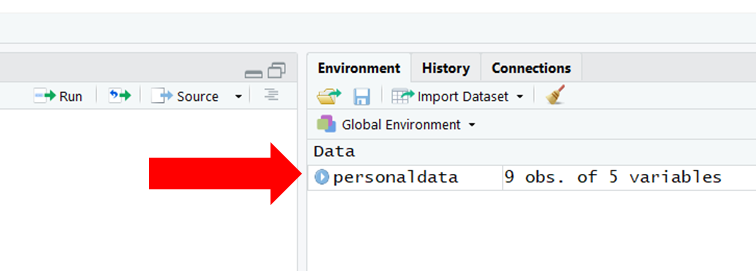
\includegraphics{dfobject.png}
\caption{}
\end{figure}

Alternatively, you can use the \texttt{View} function from base R with
the name of the data frame object we just created as the parenthetical
argument. Note that the \texttt{View} function begins with an upper-case
\texttt{V}. Remember, R is case and space sensitive when it comes to
function names. Further, the name of the data frame object you enter
into the parentheses of the function must be \emph{exactly} the same as
what you originally named the data frame object when you created it
(e.g., read it into R and named it). That is, R won't recognize the data
frame object if you type it as \texttt{PersonalData}, but R will
recognize it if you type it as \texttt{personaldata}. Sometimes it helps
to copy and paste the exact names of functions and variables into the
function parentheses.

\begin{Shaded}
\begin{Highlighting}[]
\CommentTok{# View data within data frame object}
\KeywordTok{View}\NormalTok{(personaldata)}
\end{Highlighting}
\end{Shaded}

Instead of using the \texttt{View} function, you could just ``run'' the
name of the data frame object by highlighting \texttt{personaldata} in
your R Script and clicking ``Run'' (or you can enter the name of the
data frame object directly into your Console command line and click
Enter). Another option is to use the \texttt{print} function (from base
R) with the name of the data frame object as the sole argument in the
parentheses. Similarly, if you have many rows of data, you can use the
\texttt{head} function from base R to see just the first 6 rows of data,
or you can use the \texttt{tail} function from base R to see the last 6
rows of data.

\begin{Shaded}
\begin{Highlighting}[]
\CommentTok{# Highlight the name of data frame object and click Run to view data in Console}
\NormalTok{personaldata}
\end{Highlighting}
\end{Shaded}

\begin{verbatim}
##    id   lastname firstname startdate gender
## 1 153    Sanchez Alejandro  1/1/2016   male
## 2 154   McDonald    Ronald  1/9/2016   male
## 3 155      Smith      John  1/9/2016   male
## 4 165        Doe      Jane  1/4/2016 female
## 5 125   Franklin  Benjamin  1/5/2016   male
## 6 111     Newton     Isaac  1/9/2016   male
## 7 198    Morales     Linda  1/7/2016 female
## 8 201 Providence     Cindy  1/9/2016 female
## 9 282     Legend      John  1/9/2016   male
\end{verbatim}

\begin{Shaded}
\begin{Highlighting}[]
\CommentTok{# Use print function with the name of the data frame object to view data in Console}
\KeywordTok{print}\NormalTok{(personaldata)}
\end{Highlighting}
\end{Shaded}

\begin{verbatim}
##    id   lastname firstname startdate gender
## 1 153    Sanchez Alejandro  1/1/2016   male
## 2 154   McDonald    Ronald  1/9/2016   male
## 3 155      Smith      John  1/9/2016   male
## 4 165        Doe      Jane  1/4/2016 female
## 5 125   Franklin  Benjamin  1/5/2016   male
## 6 111     Newton     Isaac  1/9/2016   male
## 7 198    Morales     Linda  1/7/2016 female
## 8 201 Providence     Cindy  1/9/2016 female
## 9 282     Legend      John  1/9/2016   male
\end{verbatim}

\begin{Shaded}
\begin{Highlighting}[]
\CommentTok{# View just the first 6 rows of the data frame object in Console}
\KeywordTok{head}\NormalTok{(personaldata)}
\end{Highlighting}
\end{Shaded}

\begin{verbatim}
##    id lastname firstname startdate gender
## 1 153  Sanchez Alejandro  1/1/2016   male
## 2 154 McDonald    Ronald  1/9/2016   male
## 3 155    Smith      John  1/9/2016   male
## 4 165      Doe      Jane  1/4/2016 female
## 5 125 Franklin  Benjamin  1/5/2016   male
## 6 111   Newton     Isaac  1/9/2016   male
\end{verbatim}

\begin{Shaded}
\begin{Highlighting}[]
\CommentTok{# View just the last 6 rows of the data frame object in Console}
\KeywordTok{tail}\NormalTok{(personaldata)}
\end{Highlighting}
\end{Shaded}

\begin{verbatim}
##    id   lastname firstname startdate gender
## 4 165        Doe      Jane  1/4/2016 female
## 5 125   Franklin  Benjamin  1/5/2016   male
## 6 111     Newton     Isaac  1/9/2016   male
## 7 198    Morales     Linda  1/7/2016 female
## 8 201 Providence     Cindy  1/9/2016 female
## 9 282     Legend      John  1/9/2016   male
\end{verbatim}

As a final note, where available, you can use the \texttt{read.csv}
function to read in .csv data from a website. For example, rather than
save the .csv file to a folder on your computer, you can read in the raw
data directly from my GitHub site. Within the quotation marks
(\texttt{"\ "}), simply paste in the following URL:
\url{https://raw.githubusercontent.com/davidcaughlin/R-Tutorial-Data-Files/master/PersData.csv}.

\begin{Shaded}
\begin{Highlighting}[]
\CommentTok{# Read data using URL}
\NormalTok{personaldata <-}\StringTok{ }\KeywordTok{read.csv}\NormalTok{(}\StringTok{"https://raw.githubusercontent.com/davidcaughlin/R-Tutorial-Data-Files/master/PersData.csv"}\NormalTok{)}
\end{Highlighting}
\end{Shaded}

Note that by naming the data frame object \texttt{personaldata} we have
overwritten the previous version of the object with that same name.

\subsection{\texorpdfstring{Option 2: \texttt{read\_csv} Function from
\texttt{readr}
Package}{Option 2: read\_csv Function from readr Package}}\label{option-2-read_csv-function-from-readr-package}

As part of the \texttt{tidyverse} of R packages
\citep{R-tidyverse, tidyverse2019}, the \texttt{readr} package
\citep{R-readr} and its functions can be used to read in a few different
data file formats (as long as they are rectangular), including .csv
files. We will use the \texttt{read\_csv} function from the package,
which as the name implies is used to read in .csv files. Among other
advantages over the \texttt{read.csv} function we learned in Option 1,
the \texttt{read\_csv} function is notably faster. Further,
\texttt{read\_csv} creates a tibble (as opposed to a data frame), which
behaves like a data frame for most purposes; for more information on
tibbles, check out Wickham and Grolemund's \citeyearpar{wickham2017}
chapter on tibbles: \url{http://r4ds.had.co.nz/tibbles.html}.

To use the \texttt{read\_csv} function, the \texttt{readr} package must
be installed and accessed using the \texttt{install.packages} and
\texttt{library} functions, respectively. Type \texttt{"readr"} (note
the quotation marks) into the parentheses of the
\texttt{install.packages} function. Next, type \texttt{readr} (without
quotation marks) into the parentheses of the \texttt{library} function.

Just like with the \texttt{read.csv} function, enter the \emph{exact}
name of the data file (as named in your working directory), followed by
.csv -- and all within quotation marks (\texttt{"\ "}). Further, either
the \texttt{\textless{}-} or \texttt{=} operator can be used to name the
data frame object. Below, I name the data frame object
\texttt{personaldata2} to distinguish it from the data frame object we
previously read in and named using the \texttt{read.csv} function.

\begin{Shaded}
\begin{Highlighting}[]
\CommentTok{# Install readr package}
\KeywordTok{install.packages}\NormalTok{(}\StringTok{"readr"}\NormalTok{)}
\end{Highlighting}
\end{Shaded}

\begin{Shaded}
\begin{Highlighting}[]
\CommentTok{# Access readr package}
\KeywordTok{library}\NormalTok{(readr)}

\CommentTok{# Read data and name data frame object}
\NormalTok{personaldata2 <-}\StringTok{ }\KeywordTok{read_csv}\NormalTok{(}\StringTok{"PersData.csv"}\NormalTok{)}
\end{Highlighting}
\end{Shaded}

\begin{verbatim}
## Parsed with column specification:
## cols(
##   id = col_double(),
##   lastname = col_character(),
##   firstname = col_character(),
##   startdate = col_character(),
##   gender = col_character()
## )
\end{verbatim}

\begin{Shaded}
\begin{Highlighting}[]
\CommentTok{# View just the first 6 rows of the data frame in Console}
\KeywordTok{head}\NormalTok{(personaldata2)}
\end{Highlighting}
\end{Shaded}

\begin{verbatim}
## # A tibble: 6 x 5
##      id lastname firstname startdate gender
##   <dbl> <chr>    <chr>     <chr>     <chr> 
## 1   153 Sanchez  Alejandro 1/1/2016  male  
## 2   154 McDonald Ronald    1/9/2016  male  
## 3   155 Smith    John      1/9/2016  male  
## 4   165 Doe      Jane      1/4/2016  female
## 5   125 Franklin Benjamin  1/5/2016  male  
## 6   111 Newton   Isaac     1/9/2016  male
\end{verbatim}

Where available, you can also use the \texttt{read\_csv} function to
read in .csv data from a website. For example, rather than save the .csv
file to a folder on your computer, you can read in the raw data directly
from my GitHub site. Within the quotation marks (\texttt{"\ "}), simply
paste in the following URL:
\url{https://raw.githubusercontent.com/davidcaughlin/R-Tutorial-Data-Files/master/PersData.csv}.

\begin{Shaded}
\begin{Highlighting}[]
\CommentTok{# Read data using URL}
\NormalTok{personaldata2 <-}\StringTok{ }\KeywordTok{read_csv}\NormalTok{(}\StringTok{"https://raw.githubusercontent.com/davidcaughlin/R-Tutorial-Data-Files/master/PersData.csv"}\NormalTok{)}
\end{Highlighting}
\end{Shaded}

\begin{verbatim}
## Parsed with column specification:
## cols(
##   id = col_double(),
##   lastname = col_character(),
##   firstname = col_character(),
##   startdate = col_character(),
##   gender = col_character()
## )
\end{verbatim}

Note that by naming the data frame object \texttt{personaldata2} we have
overwritten the previous version of the object with that same name.

\subsection{\texorpdfstring{Option 3: \texttt{Read} Function from
\texttt{lessR}
Package}{Option 3: Read Function from lessR Package}}\label{option-3-read-function-from-lessr-package}

Just like the \texttt{read.csv} and \texttt{read\_csv} functions, the
\texttt{Read} function from the \texttt{lessR} package
\citep{R-lessR2020} can read in .csv files; however, it can also read in
other file formats like .xls/x, .sas7bdat (SAS), and .sav (SPSS). When
reading in a .csv file using the \texttt{Read} function, the
\emph{exact} name of your data file from your working directory needs to
be entered as an argument (followed by .csv and surrounded by quotation
marks). Further, either the \texttt{\textless{}-} or \texttt{=} operator
can be used to name the data frame object. To use the \texttt{Read}
function, the \texttt{lessR} package needs to be installed and accessed
using the \texttt{install.packages} and \texttt{library} functions,
respectively.

\begin{Shaded}
\begin{Highlighting}[]
\CommentTok{# Install lessR package}
\KeywordTok{install.packages}\NormalTok{(}\StringTok{"lessR"}\NormalTok{)}
\end{Highlighting}
\end{Shaded}

\begin{Shaded}
\begin{Highlighting}[]
\CommentTok{# Access lessR package}
\KeywordTok{library}\NormalTok{(lessR)}

\CommentTok{# Read data and name data frame object}
\NormalTok{personaldata3 <-}\StringTok{ }\KeywordTok{Read}\NormalTok{(}\StringTok{"PersData.csv"}\NormalTok{)}
\end{Highlighting}
\end{Shaded}

\begin{verbatim}
## 
## >>> Suggestions
## To read a csv or Excel file of variable labels, var_labels=TRUE
##    Each row of the file:  Variable Name, Variable Label
## Details about your data, Enter:  details()  for d, or  details(name)
## 
## Data Types
## ------------------------------------------------------------
## character: Non-numeric data values
## integer: Numeric data values, integers only
## ------------------------------------------------------------
## 
##      Variable                  Missing  Unique 
##          Name     Type  Values  Values  Values   First and last values
## ------------------------------------------------------------------------------------------
##  1         id   integer      9       0       9   153  154  155 ... 198  201  282
##  2   lastname character      9       0       9   Sanchez  McDonald ... Providence  Legend
##  3  firstname character      9       0       8   Alejandro  Ronald ... Cindy  John
##  4  startdate character      9       0       5   1/1/2016  1/9/2016 ... 1/9/2016  1/9/2016
##  5     gender character      9       0       2   male  male  male ... female  female  male
## ------------------------------------------------------------------------------------------
\end{verbatim}

\begin{Shaded}
\begin{Highlighting}[]
\CommentTok{# View just the first 6 rows of the data frame object in Console}
\KeywordTok{head}\NormalTok{(personaldata3)}
\end{Highlighting}
\end{Shaded}

\begin{verbatim}
##    id lastname firstname startdate gender
## 1 153  Sanchez Alejandro  1/1/2016   male
## 2 154 McDonald    Ronald  1/9/2016   male
## 3 155    Smith      John  1/9/2016   male
## 4 165      Doe      Jane  1/4/2016 female
## 5 125 Franklin  Benjamin  1/5/2016   male
## 6 111   Newton     Isaac  1/9/2016   male
\end{verbatim}

Where available, you can also use the \texttt{Read} function to read in
data from a website. For example, rather than save the .csv file to a
folder on your computer, you can read in the raw data directly from my
GitHub site. Within the quotation marks (\texttt{"\ "}), simply paste in
the following URL:
\url{https://raw.githubusercontent.com/davidcaughlin/R-Tutorial-Data-Files/master/PersData.csv}.

\begin{Shaded}
\begin{Highlighting}[]
\CommentTok{# Read data using URL}
\NormalTok{personaldata3 <-}\StringTok{ }\KeywordTok{Read}\NormalTok{(}\StringTok{"https://raw.githubusercontent.com/davidcaughlin/R-Tutorial-Data-Files/master/PersData.csv"}\NormalTok{)}
\end{Highlighting}
\end{Shaded}

\begin{verbatim}
## 
## >>> Suggestions
## To read a csv or Excel file of variable labels, var_labels=TRUE
##    Each row of the file:  Variable Name, Variable Label
## Details about your data, Enter:  details()  for d, or  details(name)
## 
## Data Types
## ------------------------------------------------------------
## character: Non-numeric data values
## integer: Numeric data values, integers only
## ------------------------------------------------------------
## 
##      Variable                  Missing  Unique 
##          Name     Type  Values  Values  Values   First and last values
## ------------------------------------------------------------------------------------------
##  1         id   integer      9       0       9   153  154  155 ... 198  201  282
##  2   lastname character      9       0       9   Sanchez  McDonald ... Providence  Legend
##  3  firstname character      9       0       8   Alejandro  Ronald ... Cindy  John
##  4  startdate character      9       0       5   1/1/2016  1/9/2016 ... 1/9/2016  1/9/2016
##  5     gender character      9       0       2   male  male  male ... female  female  male
## ------------------------------------------------------------------------------------------
\end{verbatim}

Note that by naming the data frame object \texttt{personaldata3} we have
overwritten the previous version of the object with that same name.

For more information on the \texttt{Read} function from the
\texttt{lessR} package, check out David Gerbing's website for the
package and specifically the section with links to video tutorials:
\url{http://www.lessrstats.com/videos.html}.

\subsection{\texorpdfstring{Option 4: \texttt{read\_excel} Function from
\texttt{readxl}
Package}{Option 4: read\_excel Function from readxl Package}}\label{option-4-read_excel-function-from-readxl-package}

Reading in Excel workbook files with more than one worksheet requires a
bit more work. To read in a .xlsx file with two worksheets, we will use
the \texttt{excel\_sheets} and \texttt{read\_excel} functions from the
\texttt{readxl} package \citep{R-readxl}.

\begin{Shaded}
\begin{Highlighting}[]
\CommentTok{# Install readxl package}
\KeywordTok{install.packages}\NormalTok{(}\StringTok{"readxl"}\NormalTok{)}
\end{Highlighting}
\end{Shaded}

\begin{Shaded}
\begin{Highlighting}[]
\CommentTok{# Access readxl package}
\KeywordTok{library}\NormalTok{(readxl)}
\end{Highlighting}
\end{Shaded}

To view the worksheets within an Excel workbook file, simply type the
name of the \texttt{excel\_sheets} function, and as the sole
parenthetical argument type the exact name of the data file with the
.xlsx extension -- all within quotation marks (i.e.,
``PersData\_Excel.xlsx'').

\begin{Shaded}
\begin{Highlighting}[]
\CommentTok{# View Excel file worksheets}
\KeywordTok{excel_sheets}\NormalTok{(}\StringTok{"PersData_Excel.xlsx"}\NormalTok{)}
\end{Highlighting}
\end{Shaded}

\begin{verbatim}
## [1] "Year1" "Year2"
\end{verbatim}

Note that the .xlsx file contains two worksheets called ``Year1'' and
``Year2''. We can now reference each of these worksheets when reading in
the data from the Excel workbook file. To do so, we will use the
\texttt{read\_excel} function. As the first argument, enter the
\emph{exact} name of the data file (as named in your working directory),
followed by .xlsx -- and all within quotation marks (\texttt{"\ "}). As
the second argument, type \texttt{sheets=} followed by the name of the
worksheet containing the data you wish to read in; let's read in the
data from the worksheet called ``Year1''. Finally, either the
\texttt{\textless{}-} or \texttt{=} operator can be used to name the
data frame object. Below, I name the data frame object
\texttt{personaldata4}. \emph{Remember to type a comma (\texttt{,})
before the second argument, as this is how we separate arguments from
one another when there are more than one.}

\begin{Shaded}
\begin{Highlighting}[]
\CommentTok{# Read data from sheet called "Year1" and name data frame object}
\NormalTok{personaldata4 <-}\StringTok{ }\KeywordTok{read_excel}\NormalTok{(}\StringTok{"H:/RWorkshop/PersData_Excel.xlsx"}\NormalTok{, }\DataTypeTok{sheet=}\StringTok{"Year1"}\NormalTok{)}
\end{Highlighting}
\end{Shaded}

\begin{Shaded}
\begin{Highlighting}[]
\CommentTok{# View the data frame object in Console}
\KeywordTok{print}\NormalTok{(personaldata4)}
\end{Highlighting}
\end{Shaded}

\begin{verbatim}
## # A tibble: 9 x 5
##      id lastname   firstname startdate           gender
##   <dbl> <chr>      <chr>     <dttm>              <chr> 
## 1   153 Sanchez    Alejandro 2016-01-01 00:00:00 male  
## 2   154 McDonald   Ronald    2016-01-09 00:00:00 male  
## 3   155 Smith      John      2016-01-09 00:00:00 male  
## 4   165 Doe        Jane      2016-01-04 00:00:00 female
## 5   125 Franklin   Benjamin  2016-01-05 00:00:00 male  
## 6   111 Newton     Isaac     2016-01-09 00:00:00 male  
## 7   198 Morales    Linda     2016-01-07 00:00:00 female
## 8   201 Providence Cindy     2016-01-09 00:00:00 female
## 9   282 Legend     John      2016-01-09 00:00:00 male
\end{verbatim}

Let's repeat the process for the worksheet called ``Year2''.

\begin{Shaded}
\begin{Highlighting}[]
\CommentTok{# Read data from sheet called "Year2" and name data frame object}
\NormalTok{personaldata5 <-}\StringTok{ }\KeywordTok{read_excel}\NormalTok{(}\StringTok{"H:/RWorkshop/PersData_Excel.xlsx"}\NormalTok{, }\DataTypeTok{sheet=}\StringTok{"Year2"}\NormalTok{)}
\end{Highlighting}
\end{Shaded}

\begin{Shaded}
\begin{Highlighting}[]
\CommentTok{# View the data frame object in Console}
\KeywordTok{print}\NormalTok{(personaldata5)}
\end{Highlighting}
\end{Shaded}

\begin{verbatim}
## # A tibble: 9 x 5
##      id lastname   firstname startdate           gender
##   <dbl> <chr>      <chr>     <dttm>              <chr> 
## 1   153 Sanchez    Alejandro 2016-01-01 00:00:00 male  
## 2   155 Smith      John      2016-01-09 00:00:00 male  
## 3   165 Doe        Jane      2016-01-04 00:00:00 female
## 4   125 Franklin   Benjamin  2016-01-05 00:00:00 male  
## 5   111 Newton     Isaac     2016-01-09 00:00:00 male  
## 6   201 Providence Cindy     2016-01-09 00:00:00 female
## 7   282 Legend     John      2016-01-09 00:00:00 male  
## 8   312 Ramos      Jorge     2017-03-01 00:00:00 male  
## 9   395 Lucas      Nadia     2017-03-04 00:00:00 female
\end{verbatim}

\section{Special Topics}\label{special-topics}

Thus far in this chapter, I have showcased some of the most common
approaches to reading in data files, with an emphasis on reading in .csv
files with the first row corresponding to the column (variable) names
and the remaining rows containing the substantive data for cases. There
are, however, other challenges and considerations you might encounter
along the way, and this section, I cover some special topics related to
reading data into R.

\subsection{List Data File Names in Working
Directory}\label{list-data-file-names-in-working-directory}

If you would like to obtain the exact names of files located in a
(working) directory, the \texttt{list.files} function from base R comes
in handy. This function will return a list of all file names within a
particular directory or file names that meet a particular pattern. For
our purposes, let's identify all of the .csv data file names contained
within our current working directory. As the first argument, type
\texttt{path=} followed by the path associated with your working
directory. Second, because we are only pulling the file names associated
with .csv files, enter the argument \texttt{all.files=FALSE}. Third,
type the argument \texttt{full.names=FALSE} to indicate that we do not
want the path to precede the file names. Finally, type the argument
\texttt{pattern=".csv"} to request the names of only those file names
that match the regular expression of ``.csv'' will be returned.

\begin{Shaded}
\begin{Highlighting}[]
\CommentTok{# List data file names in working directory}
\KeywordTok{list.files}\NormalTok{(}\DataTypeTok{path=}\StringTok{"H:/RWorkshop"}\NormalTok{, }
           \DataTypeTok{all.files=}\OtherTok{FALSE}\NormalTok{, }
           \DataTypeTok{full.names=}\OtherTok{FALSE}\NormalTok{, }
           \DataTypeTok{pattern=}\StringTok{".csv"}\NormalTok{)}
\end{Highlighting}
\end{Shaded}

\begin{verbatim}
##  [1] "Aft_Monday_Week1.csv"                 
##  [2] "Aft_Tuesday_Week1.csv"                
##  [3] "Aft_Wednesday_Week1.csv"              
##  [4] "ANOVA_PerformanceMGMT.csv"            
##  [5] "Baseline.csv"                         
##  [6] "CData.csv"                            
##  [7] "ChiSquareTurnover.csv"                
##  [8] "DataCleaningExample.csv"              
##  [9] "Descriptive Statistics.csv"           
## [10] "DiffPred.csv"                         
## [11] "Edited PersData.csv"                  
## [12] "EmployeeDemographics.csv"             
## [13] "EmployeeSurveyData.csv"               
## [14] "EmployeeSurveyExample.csv"            
## [15] "Eve_Monday_Week1.csv"                 
## [16] "Eve_Tuesday_Week1.csv"                
## [17] "Eve_Wednesday_Week1.csv"              
## [18] "Headcount.csv"                        
## [19] "KruskalWallis.csv"                    
## [20] "lasso.csv"                            
## [21] "ManipulatingData.csv"                 
## [22] "MarketPayLine.csv"                    
## [23] "MarketSurveyData.csv"                 
## [24] "MMR.csv"                              
## [25] "Morn_Monday_Week1.csv"                
## [26] "Morn_Tuesday_Week1.csv"               
## [27] "Morn_Wednesday_Week1.csv"             
## [28] "Nonlinear.csv"                        
## [29] "PayDeterminants.csv"                  
## [30] "PayEquity.csv"                        
## [31] "PData.csv"                            
## [32] "PerfData.csv"                         
## [33] "PerfMgmtRewardSystemsExample.csv"     
## [34] "PersData.csv"                         
## [35] "PlannedBehavior.csv"                  
## [36] "Practice Table.csv"                   
## [37] "PredictiveAnalytics.csv"              
## [38] "PulseSurvey.csv"                      
## [39] "Regression.csv"                       
## [40] "Sample1.csv"                          
## [41] "Sample2.csv"                          
## [42] "SelectionExercise.csv"                
## [43] "Spearman.csv"                         
## [44] "Survival.csv"                         
## [45] "TrainingEval_inclass.csv"             
## [46] "TrainingEvaluation_PrePostControl.csv"
## [47] "TrainingEvaluation_PrePostOnly.csv"   
## [48] "TrainingEvaluation_ThreeGroupPost.csv"
## [49] "Turnover.csv"                         
## [50] "WilcoxonRankSum.csv"                  
## [51] "WilcoxonSignedRank.csv"
\end{verbatim}

In your Console, you should see the list of file names you requested.
You could then copy specific file names that you wish to read into R.

\subsection{Skip Rows of Data When
Reading}\label{skip-rows-of-data-when-reading}

Some survey platforms like Qualtrics allow for data to be downloaded in
.csv format; however, sometimes these platforms include variable name
and label information in the second and even third rows of data as
opposed to in just the first row. Fortunately, we can skip rows when
reading in such data files.

Let's pretend that the first row of the \textbf{``PersData.csv''} data
file contains variable names, and the second and third rows contain
variable label information and explanations. We can nest the
\texttt{read\_csv} function (see above) within the \texttt{names}
function, which will result in a vector of names from the first row of
the data file. Using the \texttt{\textless{}-} operator, let's name this
vector \texttt{var\_names} so that we can reference it in the subsequent
step.

\begin{Shaded}
\begin{Highlighting}[]
\CommentTok{# Read variable names from first row of data}
\NormalTok{var_names <-}\StringTok{ }\KeywordTok{names}\NormalTok{(}\KeywordTok{read_csv}\NormalTok{(}\StringTok{"PersData.csv"}\NormalTok{))}
\end{Highlighting}
\end{Shaded}

\begin{verbatim}
## Parsed with column specification:
## cols(
##   id = col_double(),
##   lastname = col_character(),
##   firstname = col_character(),
##   startdate = col_character(),
##   gender = col_character()
## )
\end{verbatim}

Next, using the \texttt{read\_csv} function, we will read in the data
file, skip the first three rows, and add the variable names we pulled in
the previous step. As usual, as the first argument of the
\texttt{read\_csv} function, type the exact name of the data file you
wish to read in within quotation marks (\texttt{"\ "}). As the second
argument, type \texttt{skip=3} to indicate that you wish to skip the
first three rows when reading in the data. As the third argument, type
\texttt{col\_names=} followed by the name of the \texttt{var\_names}
vector object we created in the previous step. Using the
\texttt{\textless{}-} operator, let's name this data frame object
\texttt{test}.

\begin{Shaded}
\begin{Highlighting}[]
\CommentTok{# Read data file (but skip rows 1-3) & introduce variable names}
\NormalTok{test <-}\StringTok{ }\KeywordTok{read_csv}\NormalTok{(}\StringTok{"PersData.csv"}\NormalTok{, }
                     \DataTypeTok{skip=}\DecValTok{3}\NormalTok{,}
                     \DataTypeTok{col_names=}\NormalTok{var_names)}
\end{Highlighting}
\end{Shaded}

\begin{verbatim}
## Parsed with column specification:
## cols(
##   id = col_double(),
##   lastname = col_character(),
##   firstname = col_character(),
##   startdate = col_character(),
##   gender = col_character()
## )
\end{verbatim}

Finally, let's see the fruits of our labor by printing the contents of
the \texttt{test} data frame object to our Console.

\begin{Shaded}
\begin{Highlighting}[]
\CommentTok{# Print data frame object}
\KeywordTok{print}\NormalTok{(test)}
\end{Highlighting}
\end{Shaded}

\begin{verbatim}
## # A tibble: 7 x 5
##      id lastname   firstname startdate gender
##   <dbl> <chr>      <chr>     <chr>     <chr> 
## 1   155 Smith      John      1/9/2016  male  
## 2   165 Doe        Jane      1/4/2016  female
## 3   125 Franklin   Benjamin  1/5/2016  male  
## 4   111 Newton     Isaac     1/9/2016  male  
## 5   198 Morales    Linda     1/7/2016  female
## 6   201 Providence Cindy     1/9/2016  female
## 7   282 Legend     John      1/9/2016  male
\end{verbatim}

\section{Summary}\label{summary}

Reading data into R is an important first step, and often, it is the
step that causes the most problems for new R users. The
\texttt{read.csv}, \texttt{read\_csv}, and \texttt{Read} functions can
all be used to read data into R. The \texttt{read\_csv} has the
advantage of being fast, which can be helpful when reading in large data
files. The \texttt{Read} function has the advantage of being able to
read in data file formats other than .csv. With all that said, if you're
working with smaller data files in the .csv format, the
\texttt{read.csv} format typically works just fine. In all subsequent
tutorials, I use the \texttt{read\_csv} function from the \texttt{readr}
package. Finally, I also demonstrated how to read in Excel workbooks
(.xlsx) files using the \texttt{read\_excel} function as well as
introduced some special topics related to reading data into R.

\chapter{Removing and Adding Variable Names}\label{addnames}

When working with a data frame object, you may encounter situations in
which it makes sense to remove the variable names (and not the variable
data) or to add or replace variables names. In this chapter, you will
learn simple techniques for removing the variable names (i.e., column
names) from a data frame object and adding (or replacing) variable names
in a data frame object.

\subsubsection{Video Tutorial}\label{video-tutorial}

Link to Video Tutorial: XXXX

\subsubsection{Functions \& Packages
Introduced}\label{functions-packages-introduced}

\begin{longtable}[]{@{}ll@{}}
\toprule
Function & Package\tabularnewline
\midrule
\endhead
\texttt{names} & base\tabularnewline
\texttt{colnames} & base\tabularnewline
\texttt{c} & base\tabularnewline
\texttt{head} & base\tabularnewline
\bottomrule
\end{longtable}

\subsubsection{Initial Steps}\label{initial-steps}

If you haven't already, save the file called \textbf{``PersData.csv''}
into a folder that you will subsequently set as your working directory.
Your working directory will likely be different than the one shown below
(i.e., \texttt{"H:/RWorkshop"}). As a reminder, you can access all of
the data files referenced in this book by downloading them as a
compressed (zipped) folder from the my GitHub site:
\url{https://github.com/davidcaughlin/R-Tutorial-Data-Files}; once
you've followed the link to GitHub, just click ``Code'' (or
``Download'') followed by ``Download ZIP'', which will download all of
the data files referenced in this book. For the sake of parsimony, I
recommend downloading all of the data files into the same folder on your
computer, which will allow you to set that same folder as your working
directory for each of the chapters in this book.

Next, using the \texttt{setwd} function, set your working directory to
the folder in which you saved the data file for this chapter.
Alternatively, you can manually set your working directory folder in
your drop-down menus by going to \emph{Session \textgreater{} Set
Working Directory \textgreater{} Choose Directory\ldots{}}. Be sure to
create a new R script file (.R) or update an existing R script file so
that you can save your script and annotations. If you need refreshers on
how to set your working directory and how to create and save an R
script, please refer to \protect\hyperlink{setwd}{Setting a Working
Directory} and \protect\hyperlink{createRscript}{Creating \& Saving an R
Script}.

\begin{Shaded}
\begin{Highlighting}[]
\CommentTok{# Set your working directory}
\KeywordTok{setwd}\NormalTok{(}\StringTok{"H:/RWorkshop"}\NormalTok{)}
\end{Highlighting}
\end{Shaded}

Next, read in the .csv data file called \textbf{``PersData.csv''} using
your choice of read function. In this example, I use the
\texttt{read\_csv} function from the \texttt{readr} package
\citep{R-readr}. If you choose to use the \texttt{read\_csv} function,
be sure that you have installed and accessed the \texttt{readr} package
using the \texttt{install.packages} and \texttt{library} functions.
\emph{Note: You don't need to install a package every time you wish to
access it; in general, I would recommend updating a package installation
once ever 1-3 months.} For refreshers on installing packages and reading
data into R, please refer to \protect\hyperlink{packages}{Packages} and
\protect\hyperlink{read}{Reading Data into R}.

\begin{Shaded}
\begin{Highlighting}[]
\CommentTok{# Install readr package if you haven't already}
\CommentTok{# [Note: You don't need to install a package every }
\CommentTok{# time you wish to access it]}
\KeywordTok{install.packages}\NormalTok{(}\StringTok{"readr"}\NormalTok{)}
\end{Highlighting}
\end{Shaded}

\begin{Shaded}
\begin{Highlighting}[]
\CommentTok{# Access readr package}
\KeywordTok{library}\NormalTok{(readr)}

\CommentTok{# Read data and name data frame (tibble) object}
\NormalTok{personaldata <-}\StringTok{ }\KeywordTok{read_csv}\NormalTok{(}\StringTok{"PersData.csv"}\NormalTok{)}
\end{Highlighting}
\end{Shaded}

\begin{verbatim}
## Parsed with column specification:
## cols(
##   id = col_double(),
##   lastname = col_character(),
##   firstname = col_character(),
##   startdate = col_character(),
##   gender = col_character()
## )
\end{verbatim}

\begin{Shaded}
\begin{Highlighting}[]
\CommentTok{# View the names of the variables in the data frame (tibble) object}
\KeywordTok{names}\NormalTok{(personaldata)}
\end{Highlighting}
\end{Shaded}

\begin{verbatim}
## [1] "id"        "lastname"  "firstname" "startdate" "gender"
\end{verbatim}

\begin{Shaded}
\begin{Highlighting}[]
\CommentTok{# View data frame (tibble) object}
\NormalTok{personaldata}
\end{Highlighting}
\end{Shaded}

\begin{verbatim}
## # A tibble: 9 x 5
##      id lastname   firstname startdate gender
##   <dbl> <chr>      <chr>     <chr>     <chr> 
## 1   153 Sanchez    Alejandro 1/1/2016  male  
## 2   154 McDonald   Ronald    1/9/2016  male  
## 3   155 Smith      John      1/9/2016  male  
## 4   165 Doe        Jane      1/4/2016  female
## 5   125 Franklin   Benjamin  1/5/2016  male  
## 6   111 Newton     Isaac     1/9/2016  male  
## 7   198 Morales    Linda     1/7/2016  female
## 8   201 Providence Cindy     1/9/2016  female
## 9   282 Legend     John      1/9/2016  male
\end{verbatim}

As you can see from the output generated in your console, the
\texttt{personaldata} data frame object contains basic employee
demographic information. The variable names include: \texttt{id},
\texttt{lastname}, \texttt{firstname}, \texttt{startdate}, and
\texttt{gender}. *Technically, the \texttt{read\_csv} function reads in
what is called a ``tibble'' object (as opposed to a data frame object),
but for our purposes a tibble will behave similarly to a data frame. For
more information on tibbles, check out Wickham and Grolemund's
\citeyearpar{wickham2017} chapter on tibbles:
\url{http://r4ds.had.co.nz/tibbles.html.*}

\section{Remove Variable Names from a Data Frame
Object}\label{remove-variable-names-from-a-data-frame-object}

In some instances, you may wish to remove the variable names from a data
frame. For example, I sometimes write (i.e., export) a data frame object
I've been cleaning in R so that I may use the data file with the
statistical software program called Mplus \citep{mplus}. Because Mplus
does accept variable names within its data files, I may drop the
variable names from the data frame object prior to writing to my working
directory.

To remove variable names, just apply the \texttt{names} function with
the data frame name as the argument, and then use either the
\texttt{\textless{}-} operator with \texttt{NULL} to remove the variable
names.

\begin{Shaded}
\begin{Highlighting}[]
\CommentTok{# Remove variable names}
\KeywordTok{names}\NormalTok{(personaldata) <-}\StringTok{ }\OtherTok{NULL}

\CommentTok{# View just the first 6 rows of the data frame object in Console}
\KeywordTok{head}\NormalTok{(personaldata)}
\end{Highlighting}
\end{Shaded}

\begin{verbatim}
## # A tibble: 6 x 5
##   <dbl> <chr>    <chr>     <chr>    <chr> 
## 1   153 Sanchez  Alejandro 1/1/2016 male  
## 2   154 McDonald Ronald    1/9/2016 male  
## 3   155 Smith    John      1/9/2016 male  
## 4   165 Doe      Jane      1/4/2016 female
## 5   125 Franklin Benjamin  1/5/2016 male  
## 6   111 Newton   Isaac     1/9/2016 male
\end{verbatim}

As you can see, the variable names do not appear in the overwritten
\texttt{personaldata} data frame object.

\section{Add Variable Names from a Data Frame
Object}\label{add-variable-names-from-a-data-frame-object}

In other instances, you might find yourself with a dataset that lacks
variable names (or has variable names that need to be replaced), which
means that you will need to add those variable names to the data frame.

Let's work with the \texttt{personaldata} data frame object from the
previous section for practice. To add variable names, we can use the
\texttt{colnames} function from base R, and enter the name of the data
frame as the argument. Using the \texttt{\textless{}-} operator, we can
specify the variable names using the \texttt{c} (combine) function that
contains a vector of variable names in quotation marks (\texttt{"\ "})
as the arguments. \emph{Remember to type a comma (\texttt{,}) between
the function arguments, as commas are used to separate arguments from
one another when there are more than one.} Please note that the it's
important that the vector of variable names contains the same number of
names as the data frame object has columns.

\begin{Shaded}
\begin{Highlighting}[]
\CommentTok{# Add (or replace) variable names to data frame object}
\KeywordTok{colnames}\NormalTok{(personaldata) <-}\StringTok{ }\KeywordTok{c}\NormalTok{(}\StringTok{"id"}\NormalTok{, }\StringTok{"lastname"}\NormalTok{, }\StringTok{"firstname"}\NormalTok{, }\StringTok{"startdate"}\NormalTok{, }\StringTok{"gender"}\NormalTok{)}

\CommentTok{# View just the first 6 rows of data in Console}
\KeywordTok{head}\NormalTok{(personaldata)}
\end{Highlighting}
\end{Shaded}

\begin{verbatim}
## # A tibble: 6 x 5
##      id lastname firstname startdate gender
##   <dbl> <chr>    <chr>     <chr>     <chr> 
## 1   153 Sanchez  Alejandro 1/1/2016  male  
## 2   154 McDonald Ronald    1/9/2016  male  
## 3   155 Smith    John      1/9/2016  male  
## 4   165 Doe      Jane      1/4/2016  female
## 5   125 Franklin Benjamin  1/5/2016  male  
## 6   111 Newton   Isaac     1/9/2016  male
\end{verbatim}

Now the data frame object has variable names!

\section{Summary}\label{summary}

In this chapter, we reviewed how to remove and add variable names in a
data frame object.

\chapter{Writing Data from R}\label{write}

\textbf{Writing data} refers to the process of exporting data from the R
environment to a (working directory) folder. If you collaborate with
others who do not work in R, writing data will allow them to use the
data you cleaned, managed, or manipulated in the R environment in other
software programs. In this chapter, we will focus on how to write a data
frame and a table to our working directory folder as .csv files.

\subsubsection{Video Tutorial}\label{video-tutorial}

Link to Video Tutorial: \url{https://youtu.be/ORTe8vE7nzU}

\subsubsection{Functions \& Packages
Introduced}\label{functions-packages-introduced}

\begin{longtable}[]{@{}ll@{}}
\toprule
Function & Package\tabularnewline
\midrule
\endhead
\texttt{write.csv} & base\tabularnewline
\texttt{write.table} & base\tabularnewline
\texttt{table} & base\tabularnewline
\bottomrule
\end{longtable}

\subsubsection{Initial Steps}\label{initial-steps}

If you haven't already, save the file called \textbf{``PersData.csv''}
into a folder that you will subsequently set as your working directory.
Your working directory will likely be different than the one shown below
(i.e., \texttt{"H:/RWorkshop"}). As a reminder, you can access all of
the data files referenced in this book by downloading them as a
compressed (zipped) folder from the my GitHub site:
\url{https://github.com/davidcaughlin/R-Tutorial-Data-Files}; once
you've followed the link to GitHub, just click ``Code'' (or
``Download'') followed by ``Download ZIP'', which will download all of
the data files referenced in this book. For the sake of parsimony, I
recommend downloading all of the data files into the same folder on your
computer, which will allow you to set that same folder as your working
directory for each of the chapters in this book.

Next, using the \texttt{setwd} function, set your working directory to
the folder in which you saved the data file for this chapter.
Alternatively, you can manually set your working directory folder in
your drop-down menus by going to \emph{Session \textgreater{} Set
Working Directory \textgreater{} Choose Directory\ldots{}}. Be sure to
create a new R script file (.R) or update an existing R script file so
that you can save your script and annotations. If you need refreshers on
how to set your working directory and how to create and save an R
script, please refer to \protect\hyperlink{setwd}{Setting a Working
Directory} and \protect\hyperlink{createRscript}{Creating \& Saving an R
Script}.

\begin{Shaded}
\begin{Highlighting}[]
\CommentTok{# Set your working directory}
\KeywordTok{setwd}\NormalTok{(}\StringTok{"H:/RWorkshop"}\NormalTok{)}
\end{Highlighting}
\end{Shaded}

Next, read in the .csv data file called \textbf{``PersData.csv''} using
your choice of read function. In this example, I use the
\texttt{read\_csv} function from the \texttt{readr} package
\citep{R-readr}. If you choose to use the \texttt{read\_csv} function,
be sure that you have installed and accessed the \texttt{readr} package
using the \texttt{install.packages} and \texttt{library} functions.
\emph{Note: You don't need to install a package every time you wish to
access it; in general, I would recommend updating a package installation
once ever 1-3 months.} For refreshers on installing packages and reading
data into R, please refer to \protect\hyperlink{packages}{Packages} and
\protect\hyperlink{read}{Reading Data into R}.

\begin{Shaded}
\begin{Highlighting}[]
\CommentTok{# Install readr package if you haven't already}
\CommentTok{# [Note: You don't need to install a package every }
\CommentTok{# time you wish to access it]}
\KeywordTok{install.packages}\NormalTok{(}\StringTok{"readr"}\NormalTok{)}
\end{Highlighting}
\end{Shaded}

\begin{Shaded}
\begin{Highlighting}[]
\CommentTok{# Access readr package}
\KeywordTok{library}\NormalTok{(readr)}

\CommentTok{# Read data and name data frame (tibble) object}
\NormalTok{personaldata <-}\StringTok{ }\KeywordTok{read_csv}\NormalTok{(}\StringTok{"PersData.csv"}\NormalTok{)}
\end{Highlighting}
\end{Shaded}

\begin{verbatim}
## Parsed with column specification:
## cols(
##   id = col_double(),
##   lastname = col_character(),
##   firstname = col_character(),
##   startdate = col_character(),
##   gender = col_character()
## )
\end{verbatim}

\begin{Shaded}
\begin{Highlighting}[]
\CommentTok{# View the names of the variables in the data frame (tibble) object}
\KeywordTok{names}\NormalTok{(personaldata)}
\end{Highlighting}
\end{Shaded}

\begin{verbatim}
## [1] "id"        "lastname"  "firstname" "startdate" "gender"
\end{verbatim}

\begin{Shaded}
\begin{Highlighting}[]
\CommentTok{# View data frame (tibble) object}
\NormalTok{personaldata}
\end{Highlighting}
\end{Shaded}

\begin{verbatim}
## # A tibble: 9 x 5
##      id lastname   firstname startdate gender
##   <dbl> <chr>      <chr>     <chr>     <chr> 
## 1   153 Sanchez    Alejandro 1/1/2016  male  
## 2   154 McDonald   Ronald    1/9/2016  male  
## 3   155 Smith      John      1/9/2016  male  
## 4   165 Doe        Jane      1/4/2016  female
## 5   125 Franklin   Benjamin  1/5/2016  male  
## 6   111 Newton     Isaac     1/9/2016  male  
## 7   198 Morales    Linda     1/7/2016  female
## 8   201 Providence Cindy     1/9/2016  female
## 9   282 Legend     John      1/9/2016  male
\end{verbatim}

As you can see from the output generated in your console, the
\texttt{personaldata} data frame object contains basic employee
demographic information. The variable names include: \texttt{id},
\texttt{lastname}, \texttt{firstname}, \texttt{startdate}, and
\texttt{gender}. *Technically, the \texttt{read\_csv} function reads in
what is called a ``tibble'' object (as opposed to a data frame object),
but for our purposes a tibble will behave similarly to a data frame. For
more information on tibbles, check out Wickham and Grolemund's
\citeyearpar{wickham2017} chapter on tibbles:
\url{http://r4ds.had.co.nz/tibbles.html.*}

\section{Write Data Frame to Working
Directory}\label{write-data-frame-to-working-directory}

The \texttt{write.csv} function from base R can be used to write a data
frame object to your working directory or to a folder of your choosing.
Let's write the \texttt{personaldata} data frame (that we read in and
named above) to our working directory. Before doing so, however, let's
make a minor change to the data frame to illustrate a scenario in which
you clean your data in R and then write the data to a .csv file so that
a colleague can work with the data in another program. Specifically,
let's remove the \texttt{lastname} variable from the data frame. To do
so, type the name of the data frame (\texttt{personaldata}), followed by
the \texttt{\$} symbol and then the name of the variable in question
(\texttt{lastname}). Next, type the \texttt{\textless{}-} operator
followed by \texttt{NULL}. This code will remove the variable from the
data frame.

\begin{Shaded}
\begin{Highlighting}[]
\CommentTok{# Remove variable from data frame}
\NormalTok{personaldata}\OperatorTok{$}\NormalTok{lastname <-}\StringTok{ }\OtherTok{NULL}

\CommentTok{# View data frame object}
\NormalTok{personaldata}
\end{Highlighting}
\end{Shaded}

\begin{verbatim}
## # A tibble: 9 x 4
##      id firstname startdate gender
##   <dbl> <chr>     <chr>     <chr> 
## 1   153 Alejandro 1/1/2016  male  
## 2   154 Ronald    1/9/2016  male  
## 3   155 John      1/9/2016  male  
## 4   165 Jane      1/4/2016  female
## 5   125 Benjamin  1/5/2016  male  
## 6   111 Isaac     1/9/2016  male  
## 7   198 Linda     1/7/2016  female
## 8   201 Cindy     1/9/2016  female
## 9   282 John      1/9/2016  male
\end{verbatim}

As you can see in your Console output, the variable called
\texttt{lastname} is no longer present in the data frame object.

To write our ``cleaned''" data frame (\texttt{personaldata}) to our
working directory, we use the \texttt{write.csv} function from base R.
As the first argument in the parentheses, type the name of the data
frame (\texttt{personaldata}). \emph{Remember to type a comma
(\texttt{,}) before the second argument, as this is how we separate
arguments from one another when there are more than one.} As the second
argument, let's type what we want to name the file that we will create
in our working directory. Make sure that the name of the new .csv file
is in quotation marks (\texttt{"\ "}). Here, I name the new file
\textbf{``Cleaned PersData.csv''}; it is important that you keep the
.csv extension at the end of the name you provide.

\begin{Shaded}
\begin{Highlighting}[]
\CommentTok{# Write data frame to working directory}
\KeywordTok{write.csv}\NormalTok{(personaldata, }\StringTok{"Cleaned PersData.csv"}\NormalTok{)}
\end{Highlighting}
\end{Shaded}

If you go to your working directory folder, you will find the file
called \textbf{``Cleaned PersData.csv''} saved there.

We can also specify which folder that we want to write our data to using
the full path extension and what we would like to name the new .csv
file.

\begin{Shaded}
\begin{Highlighting}[]
\CommentTok{# Write data frame to folder}
\KeywordTok{write.csv}\NormalTok{(personaldata, }\StringTok{"H:/RWorkshop/Cleaned PersData2.csv"}\NormalTok{)}
\end{Highlighting}
\end{Shaded}

If you go to your working directory folder, you will find the file
called **``Cleaned PersData2.csv*``**.

\section{Write Table to Working
Directory}\label{write-table-to-working-directory}

Sometimes we work with table objects in R. If we wish to write a table
to our working directory, we can use the \texttt{write.table} function
from base R. Before doing so, we need to create a data table object as
an example, which we can do using the \texttt{table} function from base
R.

To create a table, first, come up with a name for your new table object;
in this example, I name the table \texttt{table\_example} (because I'm
so creative). Second, type the \texttt{\textless{}-} operator to the
right of your new table name to tell R that you are creating a new
object. Third, type the name of the table-creation function, which is
\texttt{table}. Fourth, in the function's parentheses, as the first
argument, enter the name of first variable you wish to use to make the
table, and use the \texttt{\$} symbol to indicate that the variable
(\texttt{gender}) belongs to the data frame in question
(\texttt{personaldata}), which should look like this:
\texttt{personaldata\$gender}. Fifth, as the second argument, enter the
name of the second variable you wish to use to make the table, and use
the \texttt{\$} symbol to indicate that the variable
(\texttt{startdate}) belongs to the data frame in question
(\texttt{personaldata}), which should look like this:
\texttt{personaldata\$startdate}.

\begin{Shaded}
\begin{Highlighting}[]
\CommentTok{# Create table from gender and startdate variables from personaldata data frame}
\NormalTok{table_example <-}\StringTok{ }\KeywordTok{table}\NormalTok{(personaldata}\OperatorTok{$}\NormalTok{gender, personaldata}\OperatorTok{$}\NormalTok{startdate)}

\CommentTok{# View table in Console}
\NormalTok{table_example}
\end{Highlighting}
\end{Shaded}

\begin{verbatim}
##         
##          1/1/2016 1/4/2016 1/5/2016 1/7/2016 1/9/2016
##   female        0        1        0        1        1
##   male          1        0        1        0        4
\end{verbatim}

The table above shows how how many female versus male employees started
working on a given date.

Now we are ready to write the table called \texttt{table\_example} to
our working directory using the \texttt{write.table} function. As the
first argument, type the name of the table object
(\texttt{table\_example}). Second, type what we would like to call the
file when it is saved in our working directory
(\texttt{**"Practice\ Table.csv"**}); be sure to include the .csv
extension in the name and wrap it all in quotation marks. Third, use the
\texttt{sep=","} argument to specify that the values in the table are
separated by commas, as this will be a comma separated values file.
Fourth, add the argument \texttt{col.names=NA} to format the table such
that the column names will be aligned with their respective values. The
reason for this fourth argument is that in our table the first column
will contain the row names of one of the variables; if we don't include
this argument, the function will by default enter the name of the first
column name associated with one of the levels of the variables in the
first column, and because the first column actually contains the row
names for the table, the row names will be off by one column. The
\texttt{col.names=NA} argument simply leaves the first cell in the top
row blank so that in the next column to the right, the first column name
for one of the variables will appear. {[}To understand what the table
would look like \emph{without} this fourth argument, simply omit it, and
open the resulting file in your working directory to see what
happens.{]}

\begin{Shaded}
\begin{Highlighting}[]
\CommentTok{# Write table to working directory}
\KeywordTok{write.table}\NormalTok{(table_example, }\StringTok{"Practice Table.csv"}\NormalTok{, }\DataTypeTok{sep=}\StringTok{","}\NormalTok{, }\DataTypeTok{col.names=}\OtherTok{NA}\NormalTok{)}
\end{Highlighting}
\end{Shaded}

If you go to your working directory, you will find the file called
\textbf{``Practice Table.csv''}.

\section{Summary}\label{summary}

Writing data from the R environment to your working directory or another
folder can be useful, especially when collaborating with those who do
not use R. The \texttt{write.csv} function writes a data frame object to
a .csv file, whereas the \texttt{write.table} function writes a data
table object to a .csv file.

\part{Data Management}\label{part-data-management}

\hypertarget{arrange}{\chapter{Arranging (Sorting) Data}\label{arrange}}

\textbf{Arranging (sorting) data} refers to the process of ordering rows
numerically or alphabetically in a data frame by the values of one or
more variables. When sorting data in R, the underlying source data file
does not change; rather, the data frame object in the R Global
Environment changes. Sorting can make it easier to visually scan raw
data, particularly when used in conjunction with the \texttt{View},
\texttt{head}, or \texttt{tail} functions from base R.

\subsubsection{Video Tutorial}\label{video-tutorial}

Link to Video Tutorial: \url{https://youtu.be/wVwJQsLNbmw}

\subsubsection{Functions \& Packages
Introduced}\label{functions-packages-introduced}

\begin{longtable}[]{@{}ll@{}}
\toprule
Function & Package\tabularnewline
\midrule
\endhead
\texttt{arrange} & \texttt{dplyr}\tabularnewline
\texttt{desc} & \texttt{dplyr}\tabularnewline
\texttt{order} & base\tabularnewline
\texttt{c} & base\tabularnewline
\bottomrule
\end{longtable}

\hypertarget{initsteps_arrange}{\subsubsection{Initial
Steps}\label{initsteps_arrange}}

Please note, that any function that appears in the \emph{Initial Steps}
section has been covered in a previous chapter. If you need a refresher,
please view the relevant chapter. In addition, a previous chapter may
show you how to perform the same action using different functions or
packages.

If you haven't already, save the file called \textbf{``PersData.csv''}
into a folder that you will subsequently set as your working directory.
Your working directory will likely be different than the one shown below
(i.e., \texttt{"H:/RWorkshop"}). As a reminder, you can access all of
the data files referenced in this book by downloading them as a
compressed (zipped) folder from the my GitHub site:
\url{https://github.com/davidcaughlin/R-Tutorial-Data-Files}; once
you've followed the link to GitHub, just click ``Code'' (or
``Download'') followed by ``Download ZIP'', which will download all of
the data files referenced in this book. For the sake of parsimony, I
recommend downloading all of the data files into the same folder on your
computer, which will allow you to set that same folder as your working
directory for each of the chapters in this book.

Next, using the \texttt{setwd} function, set your working directory to
the folder in which you saved the data file for this chapter.
Alternatively, you can manually set your working directory folder in
your drop-down menus by going to \emph{Session \textgreater{} Set
Working Directory \textgreater{} Choose Directory\ldots{}}. Be sure to
create a new R script file (.R) or update an existing R script file so
that you can save your script and annotations. If you need refreshers on
how to set your working directory and how to create and save an R
script, please refer to \protect\hyperlink{setwd}{Setting a Working
Directory} and \protect\hyperlink{createRscript}{Creating \& Saving an R
Script}.

\begin{Shaded}
\begin{Highlighting}[]
\CommentTok{# Set your working directory}
\KeywordTok{setwd}\NormalTok{(}\StringTok{"H:/RWorkshop"}\NormalTok{)}
\end{Highlighting}
\end{Shaded}

Next, read in the .csv data file called \textbf{``PersData.csv''} using
your choice of read function. In this example, I use the
\texttt{read\_csv} function from the \texttt{readr} package
\citep{R-readr}. If you choose to use the \texttt{read\_csv} function,
be sure that you have installed and accessed the \texttt{readr} package
using the \texttt{install.packages} and \texttt{library} functions.
\emph{Note: You don't need to install a package every time you wish to
access it; in general, I would recommend updating a package installation
once ever 1-3 months.} For refreshers on installing packages and reading
data into R, please refer to \protect\hyperlink{packages}{Packages} and
\protect\hyperlink{read}{Reading Data into R}.

\begin{Shaded}
\begin{Highlighting}[]
\CommentTok{# Install readr package if you haven't already}
\CommentTok{# [Note: You don't need to install a package every }
\CommentTok{# time you wish to access it]}
\KeywordTok{install.packages}\NormalTok{(}\StringTok{"readr"}\NormalTok{)}
\end{Highlighting}
\end{Shaded}

\begin{Shaded}
\begin{Highlighting}[]
\CommentTok{# Access readr package}
\KeywordTok{library}\NormalTok{(readr)}

\CommentTok{# Read data and name data frame (tibble) object}
\NormalTok{personaldata <-}\StringTok{ }\KeywordTok{read_csv}\NormalTok{(}\StringTok{"PersData.csv"}\NormalTok{)}
\end{Highlighting}
\end{Shaded}

\begin{verbatim}
## Parsed with column specification:
## cols(
##   id = col_double(),
##   lastname = col_character(),
##   firstname = col_character(),
##   startdate = col_character(),
##   gender = col_character()
## )
\end{verbatim}

\begin{Shaded}
\begin{Highlighting}[]
\CommentTok{# View the names of the variables in the data frame (tibble) object}
\KeywordTok{names}\NormalTok{(personaldata)}
\end{Highlighting}
\end{Shaded}

\begin{verbatim}
## [1] "id"        "lastname"  "firstname" "startdate" "gender"
\end{verbatim}

\begin{Shaded}
\begin{Highlighting}[]
\CommentTok{# View data frame (tibble) object}
\NormalTok{personaldata}
\end{Highlighting}
\end{Shaded}

\begin{verbatim}
## # A tibble: 9 x 5
##      id lastname   firstname startdate gender
##   <dbl> <chr>      <chr>     <chr>     <chr> 
## 1   153 Sanchez    Alejandro 1/1/2016  male  
## 2   154 McDonald   Ronald    1/9/2016  male  
## 3   155 Smith      John      1/9/2016  male  
## 4   165 Doe        Jane      1/4/2016  female
## 5   125 Franklin   Benjamin  1/5/2016  male  
## 6   111 Newton     Isaac     1/9/2016  male  
## 7   198 Morales    Linda     1/7/2016  female
## 8   201 Providence Cindy     1/9/2016  female
## 9   282 Legend     John      1/9/2016  male
\end{verbatim}

As you can see from the output generated in your console, the
\texttt{personaldata} data frame object contains basic employee
demographic information. The variable names include: \texttt{id},
\texttt{lastname}, \texttt{firstname}, \texttt{startdate}, and
\texttt{gender}. Technically, the \texttt{read\_csv} function reads in
what is called a ``tibble'' object (as opposed to a data frame object),
but for our purposes a tibble will behave similarly to a data frame. For
more information on tibbles, check out Wickham and Grolemund's
\citeyearpar{wickham2017} chapter on tibbles:
\url{http://r4ds.had.co.nz/tibbles.html}.

\section{Arrange (Sort) Data}\label{arrangebyvalues}

There are different functions we could use to arrange (sort) the data in
the data frame, and in this chapter, we will focus on the
\texttt{arrange} function from the \texttt{dplyr} package
\citep{R-dplyr}. Please note that there are other functions we could use
to sort data, and if you're interested, in the
\protect\hyperlink{arrange_supplement}{Arranging (Sorting) Data: Chapter
Supplement}, I demonstrate how to use the \texttt{order} function from
base R to carry out the same operations we will cover below.

Because the \texttt{arrange} function comes from the \texttt{dplyr}
package, which is part of the \texttt{tidyverse} of R packages
\citep{R-tidyverse, tidyverse2019}. If you haven't already, install and
access the \texttt{dplyr} package using the \texttt{install.packages}
and \texttt{library} functions, respectively.

\begin{Shaded}
\begin{Highlighting}[]
\CommentTok{# Install dplyr package if you haven't already}
\CommentTok{# [Note: You don't need to install a package every }
\CommentTok{# time you wish to access it]}
\KeywordTok{install.packages}\NormalTok{(}\StringTok{"dplyr"}\NormalTok{)}
\end{Highlighting}
\end{Shaded}

\begin{Shaded}
\begin{Highlighting}[]
\CommentTok{# Access dplyr package}
\KeywordTok{library}\NormalTok{(dplyr)}
\end{Highlighting}
\end{Shaded}

Before diving into arranging the data, as a disclaimer, I will
demonstrate two techniques for arranging (sorting) data using the
\texttt{arrange} function.

The \emph{first technique} uses a ``pipe'' which in R is represented by
the \texttt{\%\textgreater{}\%} operator. The pipe operator comes from a
package called \texttt{magrittr} \citep{R-magrittr}, on which the
\texttt{dplyr} is partially dependent. In short, a pipe allows a person
to more efficiently write code and to improve the readability of the
code and overall script. Specifically, a \textbf{pipe} forwards the
result or value of one object or expression to a subsequent function. In
doing so, one can avoid writing functions in which other functions are
nested parenthetically. For more information on the pipe operator, check
out Wickham and Grolemund's \citeyearpar{wickham2017} chapter on pipes:
\url{https://r4ds.had.co.nz/pipes.html}.

This brings us to the \emph{second technique} for arranging (sorting)
data using the \texttt{arrange} function. The second technique uses a
more traditional approach that some may argue lacks the efficiency and
readability of the pipe. Conversely, others may argue against the use of
pipes altogether. I'm not here to settle any ``pipes versus no pipes''
debate, and you're welcome to use either technique. If you don't want to
learn how to use pipes (or would like to learn how to use them at a
later date), feel free to skip to the section below called
\protect\hyperlink{opt1_arrange_withoutpipe}{Without Pipe}.

\hypertarget{opt1_arrange_withpipe}{\subsection{\texorpdfstring{\emph{With}
Pipe}{With Pipe}}\label{opt1_arrange_withpipe}}

To use the ``with pipe'' technique, first, type the name of our data
frame object, which we previously named \texttt{personaldata}, followed
by the pipe (\texttt{\%\textgreater{}\%}) operator. This will ``pipe''
our data frame into the subsequent function. Second, either on the same
line or on the next line, type the name of the \texttt{arrange}
function, and within the parentheses, enter the variable name
\texttt{startdate} as the argument to indicate that we want to arrange
(sort) the data by the start date of the employees. The default
operation of the \texttt{arrange} function is to arrange (sort) the data
in \emph{ascending} order. If you're wondering where I found the exact
names of the variables in the data frame, revisit the use of the
\texttt{names} function, which I demonstrated previously in this chapter
in the \protect\hyperlink{initsteps_arrange}{Initial Steps} section.

\begin{Shaded}
\begin{Highlighting}[]
\CommentTok{# Arrange (sort) data by variable in ascending order (single line) (with pipe)}
\NormalTok{personaldata }\OperatorTok\StringTok{ }\KeywordTok{arrange}\NormalTok{(startdate)}
\end{Highlighting}
\end{Shaded}

\begin{verbatim}
## # A tibble: 9 x 5
##      id lastname   firstname startdate gender
##   <dbl> <chr>      <chr>     <chr>     <chr> 
## 1   153 Sanchez    Alejandro 1/1/2016  male  
## 2   165 Doe        Jane      1/4/2016  female
## 3   125 Franklin   Benjamin  1/5/2016  male  
## 4   198 Morales    Linda     1/7/2016  female
## 5   154 McDonald   Ronald    1/9/2016  male  
## 6   155 Smith      John      1/9/2016  male  
## 7   111 Newton     Isaac     1/9/2016  male  
## 8   201 Providence Cindy     1/9/2016  female
## 9   282 Legend     John      1/9/2016  male
\end{verbatim}

Alternatively, we can write this script over two lines and achieve the
same output in our Console.

\begin{Shaded}
\begin{Highlighting}[]
\CommentTok{# Arrange (sort) data by variable in ascending order (two lines) (with pipe)}
\NormalTok{personaldata }\OperatorTok\StringTok{ }
\StringTok{  }\KeywordTok{arrange}\NormalTok{(startdate)}
\end{Highlighting}
\end{Shaded}

\begin{verbatim}
## # A tibble: 9 x 5
##      id lastname   firstname startdate gender
##   <dbl> <chr>      <chr>     <chr>     <chr> 
## 1   153 Sanchez    Alejandro 1/1/2016  male  
## 2   165 Doe        Jane      1/4/2016  female
## 3   125 Franklin   Benjamin  1/5/2016  male  
## 4   198 Morales    Linda     1/7/2016  female
## 5   154 McDonald   Ronald    1/9/2016  male  
## 6   155 Smith      John      1/9/2016  male  
## 7   111 Newton     Isaac     1/9/2016  male  
## 8   201 Providence Cindy     1/9/2016  female
## 9   282 Legend     John      1/9/2016  male
\end{verbatim}

Please note that the operations we have performed thus far have not
changed anything in the \texttt{personaldata} data frame object itself;
rather, the output in the Console simply shows what it \emph{looks like}
if the data are sorted by the variable in question. We can verify this
by viewing the first six rows of data in our data frame object using the
\texttt{head} function. As you can see below, nothing changed in the
data frame itself.

\begin{Shaded}
\begin{Highlighting}[]
\CommentTok{# View just the first 6 rows of the data frame in Console}
\KeywordTok{head}\NormalTok{(personaldata)}
\end{Highlighting}
\end{Shaded}

\begin{verbatim}
## # A tibble: 6 x 5
##      id lastname firstname startdate gender
##   <dbl> <chr>    <chr>     <chr>     <chr> 
## 1   153 Sanchez  Alejandro 1/1/2016  male  
## 2   154 McDonald Ronald    1/9/2016  male  
## 3   155 Smith    John      1/9/2016  male  
## 4   165 Doe      Jane      1/4/2016  female
## 5   125 Franklin Benjamin  1/5/2016  male  
## 6   111 Newton   Isaac     1/9/2016  male
\end{verbatim}

To change the ordering of data in the \texttt{personaldata} data frame
object itself, we will need to (re)name the data frame object using the
\texttt{\textless{}-} variable assignment operator. In this example, I
will demonstrate how to overwrite the existing data frame object, and
thus I give the data frame object the \emph{exact} same name as it had
originally (i.e., \texttt{personaldata}). To do so, to the \emph{left}
of the \texttt{\textless{}-} operator, type what you would like to name
the new (updated) sorted data frame object (\texttt{personaldata}).
Next, to the \emph{right} of the \texttt{\textless{}-} operator, copy
and paste the same code we wrote above. Finally, use the \texttt{head}
function from base R to view the first six rows of the new data frame
object.

\begin{Shaded}
\begin{Highlighting}[]
\CommentTok{# Arrange (sort) data by variable in ascending order and }
\CommentTok{# overwrite existing data frame object (with pipe)}
\NormalTok{personaldata <-}\StringTok{ }\NormalTok{personaldata }\OperatorTok\StringTok{ }\KeywordTok{arrange}\NormalTok{(startdate)}

\CommentTok{# View just the first 6 rows of the data frame in Console}
\KeywordTok{head}\NormalTok{(personaldata)}
\end{Highlighting}
\end{Shaded}

\begin{verbatim}
## # A tibble: 6 x 5
##      id lastname firstname startdate gender
##   <dbl> <chr>    <chr>     <chr>     <chr> 
## 1   153 Sanchez  Alejandro 1/1/2016  male  
## 2   165 Doe      Jane      1/4/2016  female
## 3   125 Franklin Benjamin  1/5/2016  male  
## 4   198 Morales  Linda     1/7/2016  female
## 5   154 McDonald Ronald    1/9/2016  male  
## 6   155 Smith    John      1/9/2016  male
\end{verbatim}

As you can see in the Console output, now the \texttt{personaldata} data
frame object has been changed such that the data are arranged (sorted)
by the \texttt{startdate} variable.

To arrange the data in \emph{descending} order, just use the
\texttt{desc} function from \texttt{dplyr} within the \texttt{arrange}
function as shown below.

\begin{Shaded}
\begin{Highlighting}[]
\CommentTok{# Arrange (sort) data by variable in ascending order and }
\CommentTok{# overwrite existing data frame object (with pipe)}
\NormalTok{personaldata <-}\StringTok{ }\NormalTok{personaldata }\OperatorTok\StringTok{ }\KeywordTok{arrange}\NormalTok{(}\KeywordTok{desc}\NormalTok{(startdate))}

\CommentTok{# View just the first 6 rows of the data frame in Console}
\KeywordTok{head}\NormalTok{(personaldata)}
\end{Highlighting}
\end{Shaded}

\begin{verbatim}
## # A tibble: 6 x 5
##      id lastname   firstname startdate gender
##   <dbl> <chr>      <chr>     <chr>     <chr> 
## 1   154 McDonald   Ronald    1/9/2016  male  
## 2   155 Smith      John      1/9/2016  male  
## 3   111 Newton     Isaac     1/9/2016  male  
## 4   201 Providence Cindy     1/9/2016  female
## 5   282 Legend     John      1/9/2016  male  
## 6   198 Morales    Linda     1/7/2016  female
\end{verbatim}

To arrange (sort) data by values/levels of two variables, we simply
enter the names of two variables as consecutive arguments. Let's enter
the \texttt{gender} variable first, followed by the \texttt{startdate}
variable. The ordering of the two variables matters; the function sorts
initially by the values/levels of the first variable listed and sorts
subsequently by the values/levels of the second variable listed, but
does so \emph{within} the values/levels of the first variable listed. As
shown below, \texttt{startdate} is sorted within the sorted levels of
the \texttt{gender} variable. As a reminder, the default operation of
the \texttt{arrange} function is to arrange (sort) the data in
\emph{ascending} order. \emph{Remember, we use commas to separate
arguments used in a function (if there are more than one arguments).}

\begin{Shaded}
\begin{Highlighting}[]
\CommentTok{# Arrange (sort) data by two variables in ascending order (with pipe)}
\NormalTok{personaldata }\OperatorTok\StringTok{ }\KeywordTok{arrange}\NormalTok{(gender, startdate)}
\end{Highlighting}
\end{Shaded}

\begin{verbatim}
## # A tibble: 9 x 5
##      id lastname   firstname startdate gender
##   <dbl> <chr>      <chr>     <chr>     <chr> 
## 1   165 Doe        Jane      1/4/2016  female
## 2   198 Morales    Linda     1/7/2016  female
## 3   201 Providence Cindy     1/9/2016  female
## 4   153 Sanchez    Alejandro 1/1/2016  male  
## 5   125 Franklin   Benjamin  1/5/2016  male  
## 6   154 McDonald   Ronald    1/9/2016  male  
## 7   155 Smith      John      1/9/2016  male  
## 8   111 Newton     Isaac     1/9/2016  male  
## 9   282 Legend     John      1/9/2016  male
\end{verbatim}

Watch what happens when we switch the order of the two variables we are
using to sort the data.

\begin{Shaded}
\begin{Highlighting}[]
\CommentTok{# Arrange (sort) data by two variables in ascending order (with pipe)}
\NormalTok{personaldata }\OperatorTok\StringTok{ }\KeywordTok{arrange}\NormalTok{(startdate, gender)}
\end{Highlighting}
\end{Shaded}

\begin{verbatim}
## # A tibble: 9 x 5
##      id lastname   firstname startdate gender
##   <dbl> <chr>      <chr>     <chr>     <chr> 
## 1   153 Sanchez    Alejandro 1/1/2016  male  
## 2   165 Doe        Jane      1/4/2016  female
## 3   125 Franklin   Benjamin  1/5/2016  male  
## 4   198 Morales    Linda     1/7/2016  female
## 5   201 Providence Cindy     1/9/2016  female
## 6   154 McDonald   Ronald    1/9/2016  male  
## 7   155 Smith      John      1/9/2016  male  
## 8   111 Newton     Isaac     1/9/2016  male  
## 9   282 Legend     John      1/9/2016  male
\end{verbatim}

As you can see, the order of the two sorting variables matters.

To arrange the data in \emph{descending} order, just use the
\texttt{desc} function from \texttt{dplyr} within the \texttt{arrange}
function.

\begin{Shaded}
\begin{Highlighting}[]
\CommentTok{# Arrange (sort) data by variable in descending order (with pipe)}
\NormalTok{personaldata }\OperatorTok\StringTok{ }\KeywordTok{arrange}\NormalTok{(}\KeywordTok{desc}\NormalTok{(gender,startdate))}
\end{Highlighting}
\end{Shaded}

\begin{verbatim}
## # A tibble: 9 x 5
##      id lastname   firstname startdate gender
##   <dbl> <chr>      <chr>     <chr>     <chr> 
## 1   154 McDonald   Ronald    1/9/2016  male  
## 2   155 Smith      John      1/9/2016  male  
## 3   111 Newton     Isaac     1/9/2016  male  
## 4   282 Legend     John      1/9/2016  male  
## 5   125 Franklin   Benjamin  1/5/2016  male  
## 6   153 Sanchez    Alejandro 1/1/2016  male  
## 7   201 Providence Cindy     1/9/2016  female
## 8   198 Morales    Linda     1/7/2016  female
## 9   165 Doe        Jane      1/4/2016  female
\end{verbatim}

Or, we can sort one variable in the default ascending order and the
other in descending order.

\begin{Shaded}
\begin{Highlighting}[]
\CommentTok{# Arrange (sort) data by two variables in ascending & descending order (with pipe)}
\NormalTok{personaldata }\OperatorTok\StringTok{ }\KeywordTok{arrange}\NormalTok{(gender, }\KeywordTok{desc}\NormalTok{(startdate))}
\end{Highlighting}
\end{Shaded}

\begin{verbatim}
## # A tibble: 9 x 5
##      id lastname   firstname startdate gender
##   <dbl> <chr>      <chr>     <chr>     <chr> 
## 1   201 Providence Cindy     1/9/2016  female
## 2   198 Morales    Linda     1/7/2016  female
## 3   165 Doe        Jane      1/4/2016  female
## 4   154 McDonald   Ronald    1/9/2016  male  
## 5   155 Smith      John      1/9/2016  male  
## 6   111 Newton     Isaac     1/9/2016  male  
## 7   282 Legend     John      1/9/2016  male  
## 8   125 Franklin   Benjamin  1/5/2016  male  
## 9   153 Sanchez    Alejandro 1/1/2016  male
\end{verbatim}

\hypertarget{opt1_arrange_withoutpipe}{\subsection{\texorpdfstring{\emph{Without}
Pipe}{Without Pipe}}\label{opt1_arrange_withoutpipe}}

We can achieve the same output \emph{without} using the pipe
(\texttt{\%\textgreater{}\%}) operator as
\protect\hyperlink{opt1_arrange_withpipe}{\emph{with} the pipe
operator}; again, your choice of using or not using the pipe operator is
up to you.

To use the \texttt{arrange} function without the pipe operator, type the
name of the \texttt{arrange} function, and within the parentheses, as
the first argument, type the name of the \texttt{personaldata} data
frame object, and as the second argument, type the \texttt{startdate}
variable, where the latter indicates that we want to arrange (sort) the
data frame object by the start date of the employees. The default
operation of the \texttt{arrange} function is to arrange (sort) the data
in \emph{ascending} order. \emph{Remember, we use commas to separate
arguments used in a function (if there are more than one arguments).} If
you're wondering where I found the exact names of the variables in the
data frame, revisit the use of the \texttt{names} function, which I
demonstrated previously in this chapter in the
\protect\hyperlink{initsteps_arrange}{Initial Steps} section.

\begin{Shaded}
\begin{Highlighting}[]
\CommentTok{# Arrange (sort) data by variable in ascending order without pipe}
\KeywordTok{arrange}\NormalTok{(personaldata, startdate)}
\end{Highlighting}
\end{Shaded}

\begin{verbatim}
## # A tibble: 9 x 5
##      id lastname   firstname startdate gender
##   <dbl> <chr>      <chr>     <chr>     <chr> 
## 1   153 Sanchez    Alejandro 1/1/2016  male  
## 2   165 Doe        Jane      1/4/2016  female
## 3   125 Franklin   Benjamin  1/5/2016  male  
## 4   198 Morales    Linda     1/7/2016  female
## 5   154 McDonald   Ronald    1/9/2016  male  
## 6   155 Smith      John      1/9/2016  male  
## 7   111 Newton     Isaac     1/9/2016  male  
## 8   201 Providence Cindy     1/9/2016  female
## 9   282 Legend     John      1/9/2016  male
\end{verbatim}

To change the ordering of data in the \texttt{personaldata} data frame
object itself, we will need to (re)name the data frame object using the
\texttt{\textless{}-} variable assignment operator. In this example, I
will demonstrate how to overwrite the existing data frame object, and
thus I give the data frame object the \emph{exact} same name as it had
originally (i.e., \texttt{personaldata}). To do so, to the \emph{left}
of the \texttt{\textless{}-} operator, type what you would like to name
the new (updated) sorted data frame object (\texttt{personaldata}).
Next, to the \emph{right} of the \texttt{\textless{}-} operator, copy
and paste the same code we wrote above. Finally, use the \texttt{head}
function from base R to view the first six rows of the new data frame
object.

\begin{Shaded}
\begin{Highlighting}[]
\CommentTok{# Arrange (sort) data by variable in ascending order and }
\CommentTok{# overwrite existing data frame object without pipe}
\NormalTok{personaldata <-}\StringTok{ }\KeywordTok{arrange}\NormalTok{(personaldata, startdate)}

\CommentTok{# View just the first 6 rows of the data frame in Console}
\KeywordTok{head}\NormalTok{(personaldata)}
\end{Highlighting}
\end{Shaded}

\begin{verbatim}
## # A tibble: 6 x 5
##      id lastname firstname startdate gender
##   <dbl> <chr>    <chr>     <chr>     <chr> 
## 1   153 Sanchez  Alejandro 1/1/2016  male  
## 2   165 Doe      Jane      1/4/2016  female
## 3   125 Franklin Benjamin  1/5/2016  male  
## 4   198 Morales  Linda     1/7/2016  female
## 5   154 McDonald Ronald    1/9/2016  male  
## 6   155 Smith    John      1/9/2016  male
\end{verbatim}

To arrange the data in \emph{descending} order, just use the
\texttt{desc} function from \texttt{dplyr} within the \texttt{arrange}
function as shown below.

\begin{Shaded}
\begin{Highlighting}[]
\CommentTok{# Arrange (sort) data by variable in descending order and }
\CommentTok{# overwrite existing data frame object without pipe}
\NormalTok{personaldata <-}\StringTok{ }\KeywordTok{arrange}\NormalTok{(personaldata, }\KeywordTok{desc}\NormalTok{(startdate))}

\CommentTok{# View just the first 6 rows of the data frame in Console}
\KeywordTok{head}\NormalTok{(personaldata)}
\end{Highlighting}
\end{Shaded}

\begin{verbatim}
## # A tibble: 6 x 5
##      id lastname   firstname startdate gender
##   <dbl> <chr>      <chr>     <chr>     <chr> 
## 1   154 McDonald   Ronald    1/9/2016  male  
## 2   155 Smith      John      1/9/2016  male  
## 3   111 Newton     Isaac     1/9/2016  male  
## 4   201 Providence Cindy     1/9/2016  female
## 5   282 Legend     John      1/9/2016  male  
## 6   198 Morales    Linda     1/7/2016  female
\end{verbatim}

To arrange (sort) data by values/levels of two variables, we simply
enter the names of two variables as consecutive arguments (after the
name of the data frame, which is the first argument). Let's enter the
\texttt{gender} variable first, followed by the \texttt{startdate}
variable. The ordering of the two variables matters; the function sorts
initially by the values/levels of the first variable listed and sorts
subsequently by the values/levels of the second variable listed, but
does so \emph{within} the values/levels of the first variable listed.

\begin{Shaded}
\begin{Highlighting}[]
\CommentTok{# Arrange (sort) data by variable in ascending order without pipe}
\NormalTok{personaldata <-}\StringTok{ }\KeywordTok{arrange}\NormalTok{(personaldata, gender, startdate)}
\end{Highlighting}
\end{Shaded}

As shown in the output above, \texttt{startdate} is sorted within the
sorted levels of the \texttt{gender} variable. This also verifies that
the default operation of the \texttt{arrange} function is to arrange
(sort) the data in \emph{ascending} order.

To arrange the data in \emph{descending} order, just use the
\texttt{desc} function from \texttt{dplyr} within the \texttt{arrange}
function as shown below. You can use the \texttt{desc} function on one
or both sorting variables.

\begin{Shaded}
\begin{Highlighting}[]
\CommentTok{# Arrange (sort) data by one variable in ascending order and }
\CommentTok{# the other in descending order without pipe}
\NormalTok{personaldata <-}\StringTok{ }\KeywordTok{arrange}\NormalTok{(personaldata, gender, }\KeywordTok{desc}\NormalTok{(startdate))}
\end{Highlighting}
\end{Shaded}

Or we can apply the \texttt{desc} function to both variables.

\begin{Shaded}
\begin{Highlighting}[]
\CommentTok{# Arrange (sort) data by both variables descending order without pipe}
\NormalTok{personaldata <-}\StringTok{ }\KeywordTok{arrange}\NormalTok{(personaldata, }\KeywordTok{desc}\NormalTok{(gender, startdate))}
\end{Highlighting}
\end{Shaded}

\section{Summary}\label{summary}

In this chapter, we learned how to arrange (sort) data by one or more
variables using the \texttt{arrange} and \texttt{desc} functions from
the \texttt{dplyr} package. This chapter also introduced the pipe
(\texttt{\%\textgreater{}\%}) operator, which can help make code easier
to read in some contexts.

\hypertarget{join}{\chapter{Joining (Merging) Data}\label{join}}

\textbf{Joining} refers to the process of matching two data frames by
either one or more key variables (i.e., horizontal join) or by variable
names or columns (i.e., vertical join). Sometimes a \textbf{join} is
referred to as a \textbf{merge}, and thus I will use these terms
interchangeably. Broadly speaking, there are two types of joins
(merges): horizontal and vertical.

\subsubsection{Joining Data
Horizontally}\label{joining-data-horizontally}

A \textbf{horizontal join (merge)} refers to the process of matching
cases (i.e., rows, observations) between two data frames using a
\emph{key variable} (\emph{matching variable}), which results in
distinct sets of variables (i.e., fields, columns) being combined
horizontally (laterally) across two data frames. The resulting joined
data frame will be wider (in terms of the number of variables) than
either of the original data frames in isolation. For example, imagine
that we pull data from separate information systems, each with different
variables (i.e., fields) but at least some employees (i.e., cases) in
common; to combine these two data frames, we can perform a horizontal
join. This is often a necessary step when creating a data frame that
contains all of the variables we will need in subsequent data analyses.
For instance, if we wish to estimate the criterion-related validities
(see \protect\hyperlink{selectiontoolvalidation}{Selection Tool
Validation}) using the selection tool scores from one data frame with
criterion (e.g., job performance) scores from another data frame, then
we could perform a horizontal join.

\begin{figure}
\centering
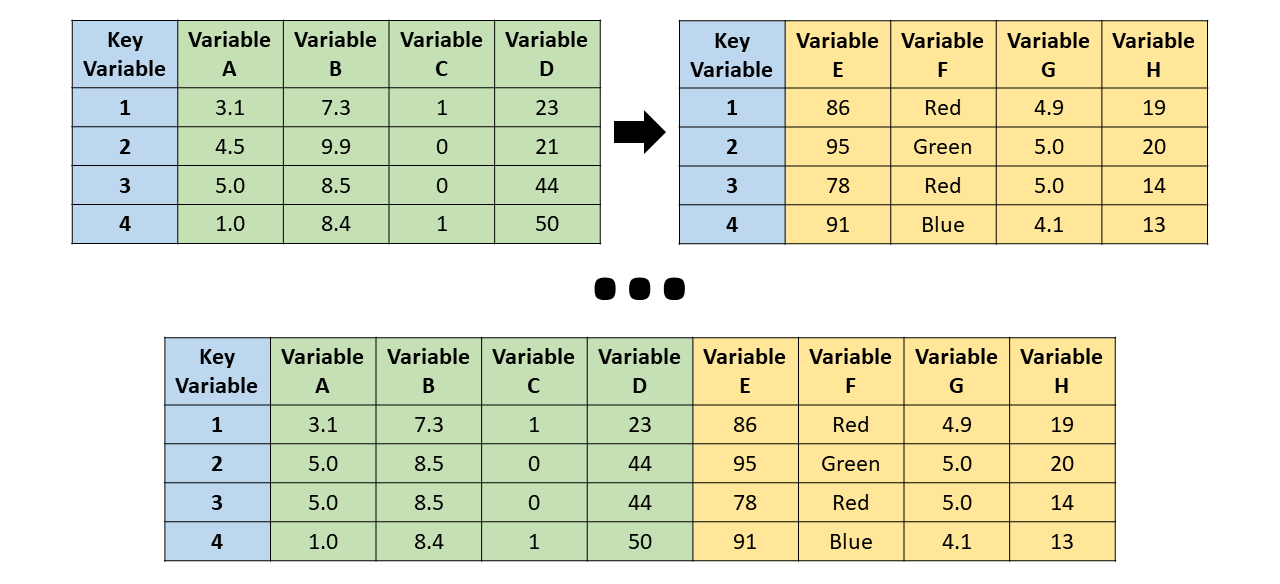
\includegraphics{horizontal_join.png}
\caption{In a \emph{horizontal join}, cases (or observations) are
matched between two data frames using one or more key variables.}
\end{figure}

We will focus on four different types of horizontal joins:

\begin{enumerate}
\def\labelenumi{\arabic{enumi}.}
\item
  Inner join
\item
  Full join
\item
  Left join
\item
  Right join
\item
  \textbf{Inner join}: All unmatched cases (or observations) are
  dropped, thereby retaining only those cases that are present in both
  the left (x, first) and right (y, second) data frames. In other words,
  a case is only included in the merged data frame if it appears in both
  of the original data data frames.
\end{enumerate}

\begin{figure}
\centering
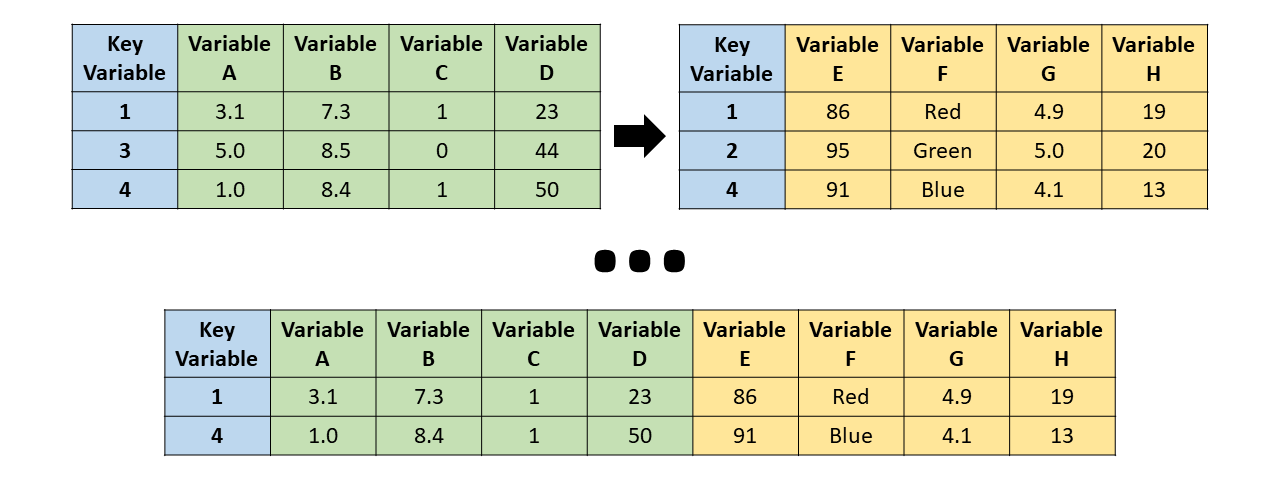
\includegraphics{inner_join.png}
\caption{In an \emph{inner join}, all unmatched cases (or observations)
are dropped, thereby retaining only those cases that are present in both
the left (x, first) and right (y, second) data frames.}
\end{figure}

\begin{enumerate}
\def\labelenumi{\arabic{enumi}.}
\setcounter{enumi}{1}
\tightlist
\item
  \textbf{Full join}: All cases (or observations) are retained,
  including those cases that do not have a match in the other data data
  frame. In other words, a case is included in the merged data frame
  even if it only appears in one of the original data data frames. These
  type of join leads to the highest number of retained cases under
  conditions in which both data frames contain unique cases.
\end{enumerate}

\begin{figure}
\centering
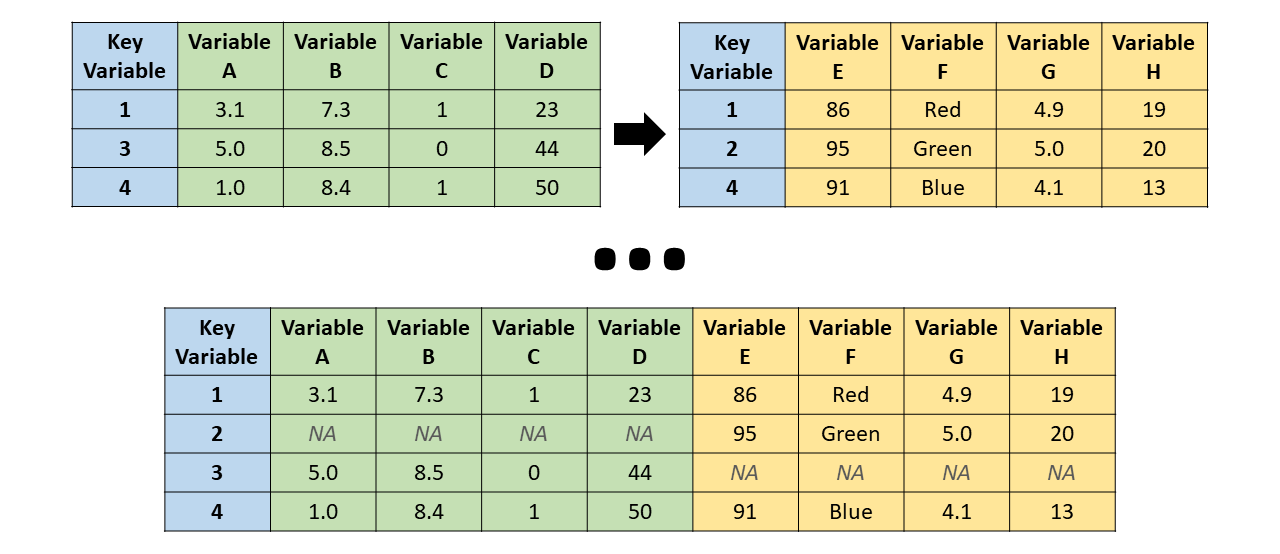
\includegraphics{full_join.png}
\caption{In a \emph{full join}, all cases (or observations) are
retained, including those cases that do not have a match in the other
data data frame.}
\end{figure}

\begin{enumerate}
\def\labelenumi{\arabic{enumi}.}
\setcounter{enumi}{2}
\tightlist
\item
  \textbf{Left join}: All cases (or observations) that appear in the
  left (x, first) data frame are retained, even if they lack a match in
  the right (y, second) data frame. Consequently, cases from the right
  data frame that lack a match in the left data frame are dropped in the
  merged data frame.
\end{enumerate}

\begin{figure}
\centering
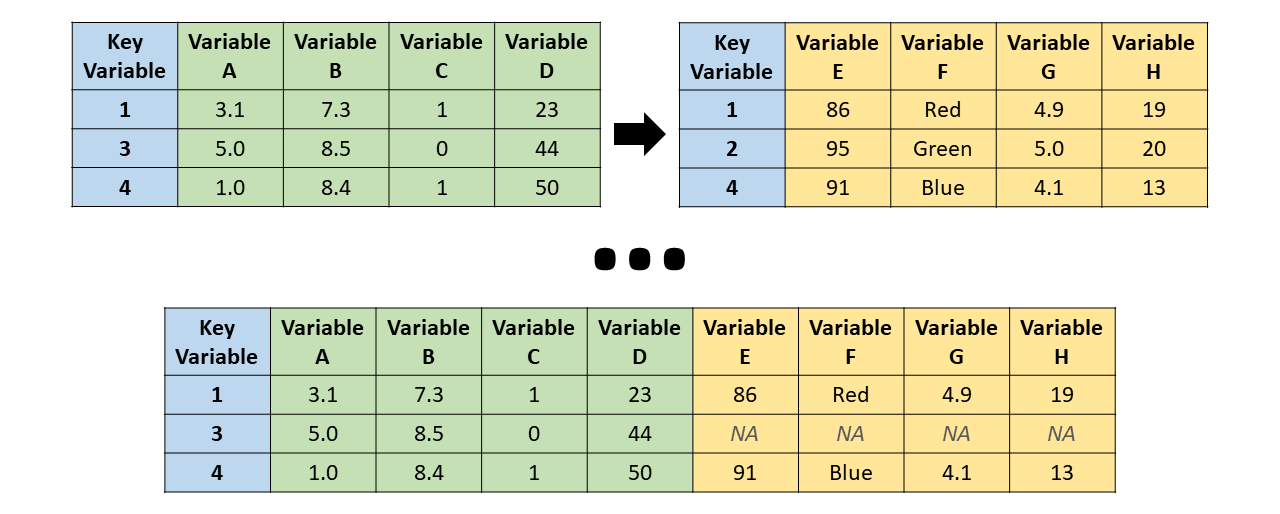
\includegraphics{left_join.png}
\caption{In a \emph{left join}, all cases (or observations) that appear
in the left (x, first) data frame are retained, even if they lack a
match in the right (y, second) data frame.}
\end{figure}

\begin{enumerate}
\def\labelenumi{\arabic{enumi}.}
\setcounter{enumi}{3}
\tightlist
\item
  \textbf{Right join}: All cases (or observations) that appear in the
  right (y, second) data frame are retained, even if they lack a match
  in the left (x, first) data frame. Consequently, cases from the left
  data frame that lack a match in the right data frame are dropped in
  the merged data frame.
\end{enumerate}

\begin{figure}
\centering
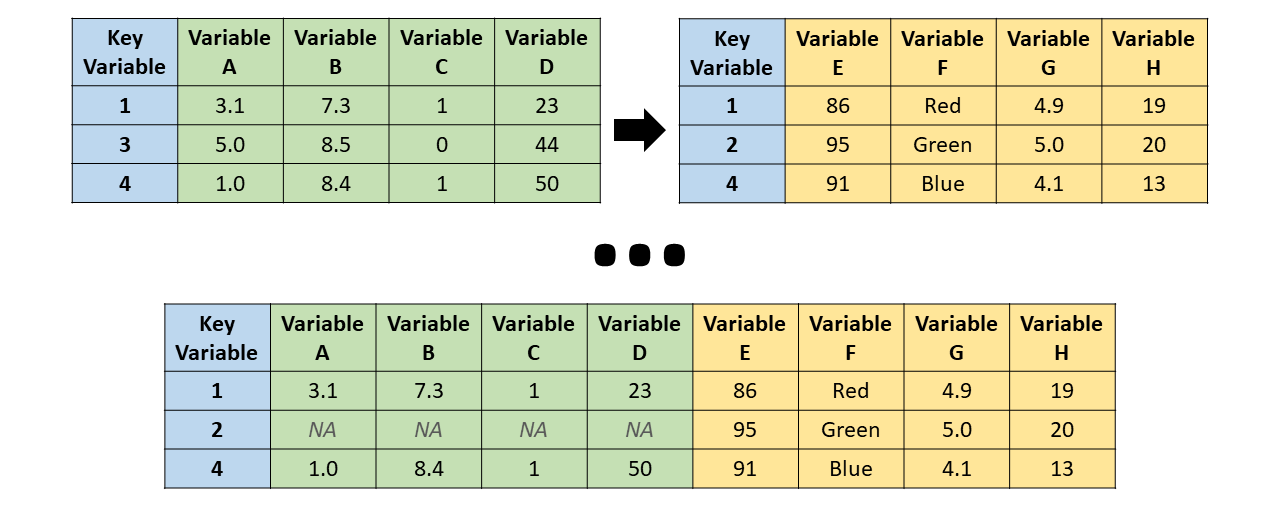
\includegraphics{right_join.png}
\caption{In a \emph{left join}, only cases (or observations) that appear
in the left (x, first) data frame are retained, even if they lack a
match in the right (y, second) data frame.}
\end{figure}

Please note that I have illustrated different types of horizontal joins
using a single key variable. It is entirely possible to perform
horizontal joins using two or more key variables. For example, imagine
that each morning we administered a pulse survey to employees and each
afternoon we afternoon we administered a different pulse survey to the
same employees, and that we repeated this process for five consecutive
workdays. In this instance, we would likely need to horizontally join
the data frames using both a unique employee identifier variable and a
unique day-of-week variable.

\subsubsection{Joining Data Vertically}\label{joining-data-vertically}

A \textbf{vertical join (merge)} refers to the process of matching
identical variables from two data frames, which results in distinct sets
of cases or observations being combined vertically. The resulting joined
data frame will be longer (in terms of the number of cases) than either
of the original data frames in isolation. For example, imagine an
organization administered the same survey to two facilities (i.e.,
independent groups) each with unique employees; we could combine the two
resulting data frames by performing a vertical join.

\begin{figure}
\centering
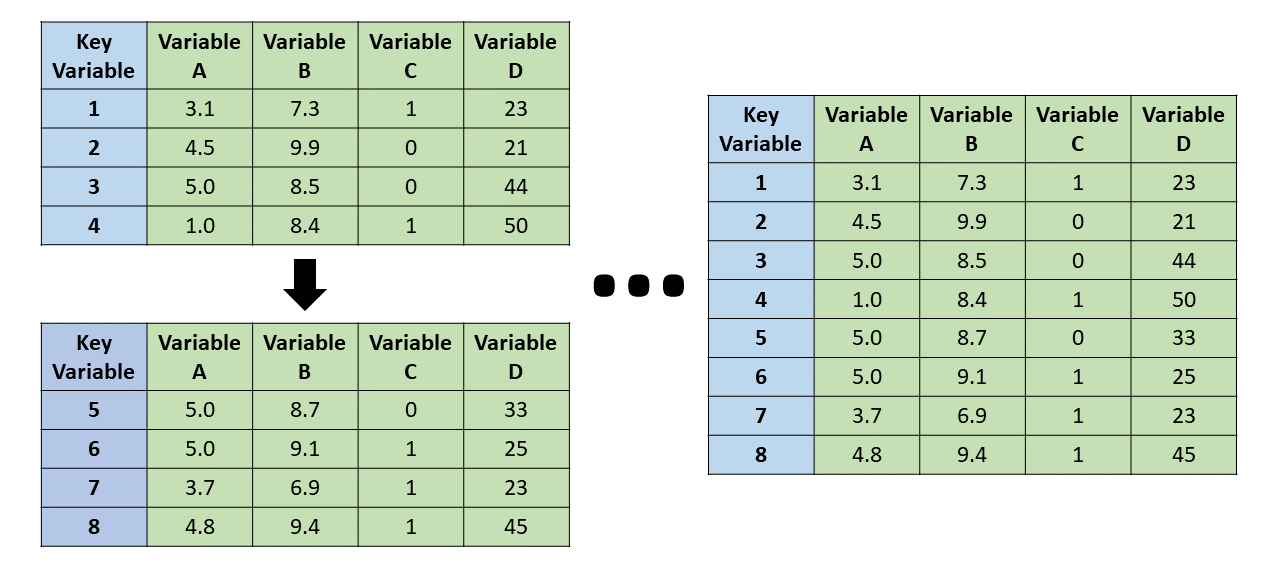
\includegraphics{vertical_join.png}
\caption{In a \emph{vertical join}, identical variables are matched
between two data frames, each with distinct sets of cases or
observations.}
\end{figure}

\subsubsection{Video Tutorial}\label{video-tutorial}

Link to Video Tutorial: \url{https://youtu.be/wVwJQsLNbmw}

\subsubsection{Functions \& Packages
Introduced}\label{functions-packages-introduced}

\begin{longtable}[]{@{}ll@{}}
\toprule
Function & Package\tabularnewline
\midrule
\endhead
\texttt{merge} & base\tabularnewline
\texttt{right\_join} & \texttt{dplyr}\tabularnewline
\texttt{left\_join} & \texttt{dplyr}\tabularnewline
\texttt{inner\_join} & \texttt{dplyr}\tabularnewline
\texttt{full\_join} & \texttt{dplyr}\tabularnewline
\texttt{data.frame} & base\tabularnewline
\texttt{c} & base\tabularnewline
\texttt{rep} & base\tabularnewline
\texttt{rbind} & base\tabularnewline
\bottomrule
\end{longtable}

\hypertarget{initsteps_join}{\subsubsection{Initial
Steps}\label{initsteps_join}}

If you haven't already, save the files called \textbf{``PersData.csv''}
and \textbf{``PerfData.csv''} into a folder that you will subsequently
set as your working directory. Your working directory will likely be
different than the one shown below (i.e., \texttt{"H:/RWorkshop"}). As a
reminder, you can access all of the data files referenced in this book
by downloading them as a compressed (zipped) folder from the my GitHub
site: \url{https://github.com/davidcaughlin/R-Tutorial-Data-Files}; once
you've followed the link to GitHub, just click ``Code'' (or
``Download'') followed by ``Download ZIP'', which will download all of
the data files referenced in this book. For the sake of parsimony, I
recommend downloading all of the data files into the same folder on your
computer, which will allow you to set that same folder as your working
directory for each of the chapters in this book.

Next, using the \texttt{setwd} function, set your working directory to
the folder in which you saved the data file for this chapter.
Alternatively, you can manually set your working directory folder in
your drop-down menus by going to \emph{Session \textgreater{} Set
Working Directory \textgreater{} Choose Directory\ldots{}}. Be sure to
create a new R script file (.R) or update an existing R script file so
that you can save your script and annotations. If you need refreshers on
how to set your working directory and how to create and save an R
script, please refer to \protect\hyperlink{setwd}{Setting a Working
Directory} and \protect\hyperlink{createRscript}{Creating \& Saving an R
Script}.

\begin{Shaded}
\begin{Highlighting}[]
\CommentTok{# Set your working directory}
\KeywordTok{setwd}\NormalTok{(}\StringTok{"H:/RWorkshop"}\NormalTok{)}
\end{Highlighting}
\end{Shaded}

Next, read in the .csv data files called \textbf{``PersData.csv''} and
\textbf{``PerfData.csv''} using your choice of read function. In this
example, I use the \texttt{read\_csv} function from the \texttt{readr}
package \citep{R-readr}. If you choose to use the \texttt{read\_csv}
function, be sure that you have installed and accessed the
\texttt{readr} package using the \texttt{install.packages} and
\texttt{library} functions. \emph{Note: You don't need to install a
package every time you wish to access it; in general, I would recommend
updating a package installation once ever 1-3 months.} For refreshers on
installing packages and reading data into R, please refer to
\protect\hyperlink{packages}{Packages} and
\protect\hyperlink{read}{Reading Data into R}.

\begin{Shaded}
\begin{Highlighting}[]
\CommentTok{# Install readr package if you haven't already}
\CommentTok{# [Note: You don't need to install a package every }
\CommentTok{# time you wish to access it]}
\KeywordTok{install.packages}\NormalTok{(}\StringTok{"readr"}\NormalTok{)}
\end{Highlighting}
\end{Shaded}

\begin{Shaded}
\begin{Highlighting}[]
\CommentTok{# Access readr package}
\KeywordTok{library}\NormalTok{(readr)}

\CommentTok{# Read data and name data frame (tibble) objects}
\NormalTok{personaldata <-}\StringTok{ }\KeywordTok{read_csv}\NormalTok{(}\StringTok{"PersData.csv"}\NormalTok{)}
\end{Highlighting}
\end{Shaded}

\begin{verbatim}
## Parsed with column specification:
## cols(
##   id = col_double(),
##   lastname = col_character(),
##   firstname = col_character(),
##   startdate = col_character(),
##   gender = col_character()
## )
\end{verbatim}

\begin{Shaded}
\begin{Highlighting}[]
\NormalTok{performancedata <-}\StringTok{ }\KeywordTok{read_csv}\NormalTok{(}\StringTok{"PerfData.csv"}\NormalTok{)}
\end{Highlighting}
\end{Shaded}

\begin{verbatim}
## Parsed with column specification:
## cols(
##   id = col_double(),
##   perf_q1 = col_double(),
##   perf_q2 = col_double(),
##   perf_q3 = col_double(),
##   perf_q4 = col_double()
## )
\end{verbatim}

\begin{Shaded}
\begin{Highlighting}[]
\CommentTok{# View the names of the variables in the data frame (tibble) objects}
\KeywordTok{names}\NormalTok{(personaldata)}
\end{Highlighting}
\end{Shaded}

\begin{verbatim}
## [1] "id"        "lastname"  "firstname" "startdate" "gender"
\end{verbatim}

\begin{Shaded}
\begin{Highlighting}[]
\KeywordTok{names}\NormalTok{(performancedata)}
\end{Highlighting}
\end{Shaded}

\begin{verbatim}
## [1] "id"      "perf_q1" "perf_q2" "perf_q3" "perf_q4"
\end{verbatim}

\begin{Shaded}
\begin{Highlighting}[]
\CommentTok{# View data frame (tibble) objects}
\NormalTok{personaldata}
\end{Highlighting}
\end{Shaded}

\begin{verbatim}
## # A tibble: 9 x 5
##      id lastname   firstname startdate gender
##   <dbl> <chr>      <chr>     <chr>     <chr> 
## 1   153 Sanchez    Alejandro 1/1/2016  male  
## 2   154 McDonald   Ronald    1/9/2016  male  
## 3   155 Smith      John      1/9/2016  male  
## 4   165 Doe        Jane      1/4/2016  female
## 5   125 Franklin   Benjamin  1/5/2016  male  
## 6   111 Newton     Isaac     1/9/2016  male  
## 7   198 Morales    Linda     1/7/2016  female
## 8   201 Providence Cindy     1/9/2016  female
## 9   282 Legend     John      1/9/2016  male
\end{verbatim}

\begin{Shaded}
\begin{Highlighting}[]
\NormalTok{performancedata}
\end{Highlighting}
\end{Shaded}

\begin{verbatim}
## # A tibble: 6 x 5
##      id perf_q1 perf_q2 perf_q3 perf_q4
##   <dbl>   <dbl>   <dbl>   <dbl>   <dbl>
## 1   153     3.9     4.8     4.9     5  
## 2   125     2.1     1.9     2.1     2.3
## 3   111     3.3     3.3     3.4     3.3
## 4   198     4.9     4.5     4.4     4.8
## 5   201     1.2     1.1     1       1  
## 6   282     2.2     2.3     2.4     2.5
\end{verbatim}

As you can see from the output generated in your console, on the one
hand, the \texttt{personaldata} data frame object contains basic
employee demographic information. The variable names include:
\texttt{id}, \texttt{lastname}, \texttt{firstname}, \texttt{startdate},
and \texttt{gender}. On the other hand, the \texttt{personaldata} data
frame object contains the same \texttt{id} unique identifer variable as
the \texttt{personaldata} data frame object, but instead of employee
demographic information, this data frame object includes varuables
associated with quarterly employee performance: \texttt{perf\_q1},
\texttt{perf\_q2}, \texttt{perf\_q3}, and \texttt{perf\_q4}.

In order to better illustrate certain join functions later on in this
chapter, we'll begin by removing the case (i.e., employee) associated
with the \texttt{id} variable value of 153 (i.e., Alejandro Sanchez); in
terms of a rationale for doing so, let's imagine that Alejandro no
longer works for the organization, and thus we would like to remove him
from the \texttt{personaldata} data frame. If you don't completely
understand the following process for removing this individual from the
data frame, no need to worry, as you will learn more in the subsequent
chapter on \protect\hyperlink{filter}{filtering data}.

\begin{enumerate}
\def\labelenumi{\arabic{enumi}.}
\tightlist
\item
  Type the name of the data frame object (\texttt{personaldata})
  followed by the \texttt{\textless{}-} operator to overwrite the
  existing data frame object.
\item
  Type the name of the original data frame object
  (\texttt{personaldata}) followed by brackets (\texttt{{[}\ {]}}).
\item
  Within the brackets (\texttt{{[}\ {]}}), type the name of the data
  frame object (\texttt{personaldata}) again, followed by the
  \texttt{\$} operator and the name of the variable we wish to use to
  select the case that will be removed, which in this instance is the
  \texttt{id} unique identifier variable. The \texttt{\$} operator
  indicates to R that the \texttt{id} variable belongs to the
  \texttt{personaldata} data frame.
\item
  Type the ``not equal to'' operator, which is \texttt{!=} (the
  \texttt{!} means ``not''), followed by the \texttt{id} variable value
  we wish to use to remove the case (i.e., 153).
\item
  Type a comma (\texttt{,}) to indicate that we are removing a row, not
  a column. \emph{When referencing rows and columns in R, as we are
  doing in the brackets (\texttt{{[}\ {]}}), rows are entered first
  (before a comma), and columns are entered second (after a comma).} In
  doing so, we are telling R to retain all rows of data in
  \texttt{personaldata} except for the one corresponding to \texttt{id}
  equal to 153.
\end{enumerate}

\begin{Shaded}
\begin{Highlighting}[]
\CommentTok{# Remove case with id variable equal to 153}
\NormalTok{personaldata <-}\StringTok{ }\NormalTok{personaldata[personaldata}\OperatorTok{$}\NormalTok{id }\OperatorTok{!=}\StringTok{ }\DecValTok{153}\NormalTok{,]}
\end{Highlighting}
\end{Shaded}

Check out the first 6 rows of the updated data frame for
\texttt{personaldata}, and note that the data corresponding to the case
associated with \texttt{id} equal to 153 is gone.

\begin{Shaded}
\begin{Highlighting}[]
\CommentTok{# View first 6 rows of first data frame object once more}
\KeywordTok{head}\NormalTok{(personaldata)}
\end{Highlighting}
\end{Shaded}

\begin{verbatim}
## # A tibble: 6 x 5
##      id lastname firstname startdate gender
##   <dbl> <chr>    <chr>     <chr>     <chr> 
## 1   154 McDonald Ronald    1/9/2016  male  
## 2   155 Smith    John      1/9/2016  male  
## 3   165 Doe      Jane      1/4/2016  female
## 4   125 Franklin Benjamin  1/5/2016  male  
## 5   111 Newton   Isaac     1/9/2016  male  
## 6   198 Morales  Linda     1/7/2016  female
\end{verbatim}

\hypertarget{horizontaljoin}{\section{Horizontal Join
(Merge)}\label{horizontaljoin}}

Recall that a horizontal join (merge) means that cases are matched using
one more more key variables, and as a result, variables (i.e., columns,
fields) are combined across two data frames. We will review two options
for performing horizontal joins.

To perform horizontal joins, we will learn how to use the \texttt{join}
functions from the the \texttt{dplyr} package \citep{R-dplyr}, which
include: \texttt{right\_join}, \texttt{left\_join},
\texttt{inner\_join}, and \texttt{full\_join}. Please note that there
are other functions we could use to perform horizontal joins, and if
you're interested, in the \protect\hyperlink{join_supplement}{Joining
(Merging) Data: Chapter Supplement}, I demonstrate how to use the
\texttt{merge} function from base R to carry out the same operations we
will cover below.

Using the aformentioned \texttt{join} functions, we will match cases
from the \texttt{personaldata} and \texttt{performancedata} data frames
using the \texttt{id} unique identifer variable as a key variable. So
how can we verify that \texttt{id} is an appropriate key variable? Well,
let's use the \texttt{names} function from base R to retrieve the list
of variable names from the two data frames, which we already did above.
Nevertheless, let's call up those variable names once more. Simply enter
the name of the data frame as a parenthetical argument in the
\texttt{names} function.

\begin{Shaded}
\begin{Highlighting}[]
\CommentTok{# Retrieve variable names from first data frame}
\KeywordTok{names}\NormalTok{(personaldata)}
\end{Highlighting}
\end{Shaded}

\begin{verbatim}
## [1] "id"        "lastname"  "firstname" "startdate" "gender"
\end{verbatim}

\begin{Shaded}
\begin{Highlighting}[]
\CommentTok{# Retrieve variable names from second data frame}
\KeywordTok{names}\NormalTok{(performancedata)}
\end{Highlighting}
\end{Shaded}

\begin{verbatim}
## [1] "id"      "perf_q1" "perf_q2" "perf_q3" "perf_q4"
\end{verbatim}

As you can see in the variable names listed above, the \texttt{id}
variable is common to both data frames, and thus it will serve as our
key variable.

Now we are almost ready to begin joining the two data frames using the
\texttt{id} unique identifer as a key variable. Before doing so,
however, we should make sure that we have installed and accessed the
\texttt{dplyr} package (if we haven't already), as the \texttt{join}
functions come from that package.

\begin{Shaded}
\begin{Highlighting}[]
\CommentTok{# Install dplyr package if you haven't already}
\CommentTok{# [Note: You don't need to install a package every }
\CommentTok{# time you wish to access it]}
\KeywordTok{install.packages}\NormalTok{(}\StringTok{"dplyr"}\NormalTok{)}
\end{Highlighting}
\end{Shaded}

\begin{Shaded}
\begin{Highlighting}[]
\CommentTok{# Access dplyr package}
\KeywordTok{library}\NormalTok{(dplyr)}
\end{Highlighting}
\end{Shaded}

I will demonstrate two techniques for applying the \texttt{join}
function.

The \emph{first technique} uses the pipe operator
(\texttt{\%\textgreater{}\%}). The pipe operator comes from a package
called \texttt{magrittr} \citep{R-magrittr}, on which the \texttt{dplyr}
is partially dependent. In short, a pipe allows a person to more
efficiently write code and to improve the readability of the code and
overall script. Specifically, a \textbf{pipe} forwards the result or
value of one object or expression to a subsequent function. In doing so,
one can avoid writing functions in which other functions are nested
parenthetically. For more information on the pipe operator, check out
Wickham and Grolemund's \citeyearpar{wickham2017} chapter on pipes:
\url{https://r4ds.had.co.nz/pipes.html}.

The \emph{second technique} for applying the \texttt{join} function
takes a more traditional approach in that it involves nested functions
being nested parenthetically. If you don't want to learn how to use
pipes (or would like to learn how to use them at a later date), feel
free to skip to the section below called
\protect\hyperlink{opt2_join_withoutpipe}{Without Pipe}.

\hypertarget{opt2_join_withpipe}{\subsection{\texorpdfstring{\emph{With}
Pipe}{With Pipe}}\label{opt2_join_withpipe}}

Using the pipe (\texttt{\%\textgreater{}\%}) operator technique, let's
begin with what is referred to as an \textbf{inner join} by doing the
following:

\begin{enumerate}
\def\labelenumi{\arabic{enumi}.}
\tightlist
\item
  Use the \texttt{\textless{}-} symbol to name the joined (merged) data
  frame that we will create using the one of the \texttt{dplyr} join
  functions. For this example, I name the new joined data frame
  \texttt{mergeddf}, which is completely arbitrary; you could name it
  whatever you would like. Make sure you put the name of the new data
  frame object to the \emph{left} of the \texttt{\textless{}-} operator.
\item
  To the \emph{right} of the \texttt{\textless{}-} operator, type the
  name of the first data frame, which we named \texttt{personaldata},
  followed by the pipe (\texttt{\%\textgreater{}\%}) operator. This will
  ``pipe'' our data frame into the subsequent function.
\item
  On the same line or on the next line, type the \texttt{inner\_join}
  function, and within the parentheses as the first argument, type the
  name of the second data frame, which we called
  \texttt{performancedata}. As the second argument, use the \texttt{by=}
  argument to indicate the name of the key variable, which in this
  example is \texttt{id}; make sure the key variable is in quotation
  marks (\texttt{"\ "}), and remember, object and variable names in R
  are case and space sensitive.
\end{enumerate}

\begin{Shaded}
\begin{Highlighting}[]
\CommentTok{# Inner join (with pipe)}
\NormalTok{mergeddf <-}\StringTok{ }\NormalTok{personaldata }\OperatorTok\StringTok{ }\KeywordTok{inner_join}\NormalTok{(performancedata, }\DataTypeTok{by=}\StringTok{"id"}\NormalTok{)}

\CommentTok{# View the joined data frame}
\NormalTok{mergeddf}
\end{Highlighting}
\end{Shaded}

\begin{verbatim}
## # A tibble: 5 x 9
##      id lastname   firstname startdate gender perf_q1 perf_q2 perf_q3 perf_q4
##   <dbl> <chr>      <chr>     <chr>     <chr>    <dbl>   <dbl>   <dbl>   <dbl>
## 1   125 Franklin   Benjamin  1/5/2016  male       2.1     1.9     2.1     2.3
## 2   111 Newton     Isaac     1/9/2016  male       3.3     3.3     3.4     3.3
## 3   198 Morales    Linda     1/7/2016  female     4.9     4.5     4.4     4.8
## 4   201 Providence Cindy     1/9/2016  female     1.2     1.1     1       1  
## 5   282 Legend     John      1/9/2016  male       2.2     2.3     2.4     2.5
\end{verbatim}

Now, let's revisit the original data frame objects that we read in
initially.

\begin{Shaded}
\begin{Highlighting}[]
\CommentTok{# View the first original data frame}
\NormalTok{personaldata}
\end{Highlighting}
\end{Shaded}

\begin{verbatim}
## # A tibble: 8 x 5
##      id lastname   firstname startdate gender
##   <dbl> <chr>      <chr>     <chr>     <chr> 
## 1   154 McDonald   Ronald    1/9/2016  male  
## 2   155 Smith      John      1/9/2016  male  
## 3   165 Doe        Jane      1/4/2016  female
## 4   125 Franklin   Benjamin  1/5/2016  male  
## 5   111 Newton     Isaac     1/9/2016  male  
## 6   198 Morales    Linda     1/7/2016  female
## 7   201 Providence Cindy     1/9/2016  female
## 8   282 Legend     John      1/9/2016  male
\end{verbatim}

\begin{Shaded}
\begin{Highlighting}[]
\CommentTok{# View the second original data frame}
\NormalTok{performancedata}
\end{Highlighting}
\end{Shaded}

\begin{verbatim}
## # A tibble: 6 x 5
##      id perf_q1 perf_q2 perf_q3 perf_q4
##   <dbl>   <dbl>   <dbl>   <dbl>   <dbl>
## 1   153     3.9     4.8     4.9     5  
## 2   125     2.1     1.9     2.1     2.3
## 3   111     3.3     3.3     3.4     3.3
## 4   198     4.9     4.5     4.4     4.8
## 5   201     1.2     1.1     1       1  
## 6   282     2.2     2.3     2.4     2.5
\end{verbatim}

In the output, first, note how all of the variables from the original
data frames (i.e., \texttt{personaldata}, \texttt{performancedata}) are
represented in the merged data frame (i.e., \texttt{mergeddf}). Second,
note how the cases are matched by the \texttt{id} key variable. Third,
note that the \texttt{personaldata} data frame has 8 cases, the
\texttt{performancedata} data frame has 6 cases, and the
\texttt{mergeddf} data frame has 6 cases. By default, the \texttt{merge}
function performs an \emph{inner join} and retains only those matched
cases that have data in \emph{both} data frames. Because cases whose
\texttt{id} values were \texttt{154}, \texttt{155}, and \texttt{165} had
data in \texttt{personaldata} but not \texttt{performancedata} and
because the case with an \texttt{id} value equal to 153 was in
\texttt{performancedata} but not \texttt{personaldata}, only the 5 cases
that had available data in both data frames were retained.

To perform what is referred to as a \textbf{full join} in which we
retain all cases and available data, we simply swap out the
\texttt{inner\_join} function from our previous code with the
\texttt{full\_join} function.

\begin{Shaded}
\begin{Highlighting}[]
\CommentTok{# Full join (with pipe)}
\NormalTok{mergeddf <-}\StringTok{ }\NormalTok{personaldata }\OperatorTok\StringTok{ }\KeywordTok{full_join}\NormalTok{(performancedata, }\DataTypeTok{by=}\StringTok{"id"}\NormalTok{)}

\CommentTok{# View the joined data frame}
\NormalTok{mergeddf}
\end{Highlighting}
\end{Shaded}

\begin{verbatim}
## # A tibble: 9 x 9
##      id lastname   firstname startdate gender perf_q1 perf_q2 perf_q3 perf_q4
##   <dbl> <chr>      <chr>     <chr>     <chr>    <dbl>   <dbl>   <dbl>   <dbl>
## 1   154 McDonald   Ronald    1/9/2016  male      NA      NA      NA      NA  
## 2   155 Smith      John      1/9/2016  male      NA      NA      NA      NA  
## 3   165 Doe        Jane      1/4/2016  female    NA      NA      NA      NA  
## 4   125 Franklin   Benjamin  1/5/2016  male       2.1     1.9     2.1     2.3
## 5   111 Newton     Isaac     1/9/2016  male       3.3     3.3     3.4     3.3
## 6   198 Morales    Linda     1/7/2016  female     4.9     4.5     4.4     4.8
## 7   201 Providence Cindy     1/9/2016  female     1.2     1.1     1       1  
## 8   282 Legend     John      1/9/2016  male       2.2     2.3     2.4     2.5
## 9   153 <NA>       <NA>      <NA>      <NA>       3.9     4.8     4.9     5
\end{verbatim}

Note how the \texttt{full\_join} function retains all available cases
that had available data in at least one of the data frames, which in
this example is 9 cases. \emph{When in doubt, I recommend using the
\texttt{full\_join} function to retain all available data.}

To perform what is referred to as a \textbf{left join} in which we
retain only those cases with data available in the first (left, x) data
frame (\texttt{personaldata}), we use the \texttt{left\_join} function
instead, while keeping the rest of the previous code the same.

\begin{Shaded}
\begin{Highlighting}[]
\CommentTok{# Left join (with pipe)}
\NormalTok{mergeddf <-}\StringTok{ }\NormalTok{personaldata }\OperatorTok\StringTok{ }\KeywordTok{left_join}\NormalTok{(performancedata, }\DataTypeTok{by=}\StringTok{"id"}\NormalTok{)}

\CommentTok{# View the joined data frame}
\NormalTok{mergeddf}
\end{Highlighting}
\end{Shaded}

\begin{verbatim}
## # A tibble: 8 x 9
##      id lastname   firstname startdate gender perf_q1 perf_q2 perf_q3 perf_q4
##   <dbl> <chr>      <chr>     <chr>     <chr>    <dbl>   <dbl>   <dbl>   <dbl>
## 1   154 McDonald   Ronald    1/9/2016  male      NA      NA      NA      NA  
## 2   155 Smith      John      1/9/2016  male      NA      NA      NA      NA  
## 3   165 Doe        Jane      1/4/2016  female    NA      NA      NA      NA  
## 4   125 Franklin   Benjamin  1/5/2016  male       2.1     1.9     2.1     2.3
## 5   111 Newton     Isaac     1/9/2016  male       3.3     3.3     3.4     3.3
## 6   198 Morales    Linda     1/7/2016  female     4.9     4.5     4.4     4.8
## 7   201 Providence Cindy     1/9/2016  female     1.2     1.1     1       1  
## 8   282 Legend     John      1/9/2016  male       2.2     2.3     2.4     2.5
\end{verbatim}

Note how the \texttt{left\_join} function retains only those cases for
which the first (left, x) data frame (i.e., \texttt{personaldata}) has
complete data, which in this case happens to be 8 cases. Notably absent
is the case associated with \texttt{id} equal to 153 because the first
(left, x) data frame (i.e., \texttt{personaldata}) lacked that case. An
\texttt{NA} appears for each case from the second (right, y) data frame
that contained missing values on variables from that data frame.

To perform what is referred to as a \textbf{right join} in which we
retain only those cases with data available in the second (right, y)
data frame (\texttt{performancedata}), we use the \texttt{right\_join}
function instead, while keeping the rest of the previous code the same.

\begin{Shaded}
\begin{Highlighting}[]
\CommentTok{# Right join (with pipe)}
\NormalTok{mergeddf <-}\StringTok{ }\NormalTok{personaldata }\OperatorTok\StringTok{ }\KeywordTok{right_join}\NormalTok{(performancedata, }\DataTypeTok{by=}\StringTok{"id"}\NormalTok{)}

\CommentTok{# View the joined data frame}
\NormalTok{mergeddf}
\end{Highlighting}
\end{Shaded}

\begin{verbatim}
## # A tibble: 6 x 9
##      id lastname   firstname startdate gender perf_q1 perf_q2 perf_q3 perf_q4
##   <dbl> <chr>      <chr>     <chr>     <chr>    <dbl>   <dbl>   <dbl>   <dbl>
## 1   125 Franklin   Benjamin  1/5/2016  male       2.1     1.9     2.1     2.3
## 2   111 Newton     Isaac     1/9/2016  male       3.3     3.3     3.4     3.3
## 3   198 Morales    Linda     1/7/2016  female     4.9     4.5     4.4     4.8
## 4   201 Providence Cindy     1/9/2016  female     1.2     1.1     1       1  
## 5   282 Legend     John      1/9/2016  male       2.2     2.3     2.4     2.5
## 6   153 <NA>       <NA>      <NA>      <NA>       3.9     4.8     4.9     5
\end{verbatim}

Note how the \texttt{right\_join} function retains only those cases for
which the joined (second, right, y) data frame (i.e.,
\texttt{performancedata}) has complete data. Because the first (left, x)
data frame lacks data for the case in which \texttt{id} is equal to 153,
an \texttt{NA} appears for each case from the first data frame that
contained missing values on variables from that data frame.

\hypertarget{opt2_join_withoutpipe}{\subsection{\texorpdfstring{\emph{Without}
Pipe}{Without Pipe}}\label{opt2_join_withoutpipe}}

In this section, I demonstrate the same \texttt{dplyr} join functions
\protect\hyperlink{opt2_join_withpipe}{as above}, except here I
demonstrate how to specify the functions \emph{without} the use of a
pipe (\texttt{\%\textgreater{}\%}) operator.

Let's begin with what is referred to as an \textbf{inner join} by doing
the following:

\begin{enumerate}
\def\labelenumi{\arabic{enumi}.}
\tightlist
\item
  Use the \texttt{\textless{}-} operator to name the joined (merged)
  data frame that we will create using the one of the \texttt{dplyr}
  join functions. For this example, I name the new joined data frame
  \texttt{mergeddf}, which is completely arbitrary; you could name it
  whatever you would like. Make sure you put the name of the new data
  frame object to the \emph{left} of the \texttt{\textless{}-} operator.
\item
  To the \emph{right} of the \texttt{\textless{}-} operator, type the
  name of the \texttt{inner\_join} function. As the first argument
  within the parentheses, type the name of the first data frame, which
  we named \texttt{personaldata}. As the second argument, type the name
  of the second data frame we named \texttt{performancedata}. As the
  third argument, use the \texttt{by=} argument to indicate the name of
  the key variable, which in this example is \texttt{id}; make sure the
  key variable is in quotation marks (\texttt{"\ "}), and remember,
  object and variable names in R are case and space sensitive.
\end{enumerate}

\begin{Shaded}
\begin{Highlighting}[]
\CommentTok{# Inner join (without pipe)}
\NormalTok{mergeddf <-}\StringTok{ }\KeywordTok{inner_join}\NormalTok{(personaldata, performancedata, }\DataTypeTok{by=}\StringTok{"id"}\NormalTok{)}

\CommentTok{# View the joined data frame}
\NormalTok{mergeddf}
\end{Highlighting}
\end{Shaded}

\begin{verbatim}
## # A tibble: 5 x 9
##      id lastname   firstname startdate gender perf_q1 perf_q2 perf_q3 perf_q4
##   <dbl> <chr>      <chr>     <chr>     <chr>    <dbl>   <dbl>   <dbl>   <dbl>
## 1   125 Franklin   Benjamin  1/5/2016  male       2.1     1.9     2.1     2.3
## 2   111 Newton     Isaac     1/9/2016  male       3.3     3.3     3.4     3.3
## 3   198 Morales    Linda     1/7/2016  female     4.9     4.5     4.4     4.8
## 4   201 Providence Cindy     1/9/2016  female     1.2     1.1     1       1  
## 5   282 Legend     John      1/9/2016  male       2.2     2.3     2.4     2.5
\end{verbatim}

Now, let's revisit the original data frame objects that we read in
initially.

\begin{Shaded}
\begin{Highlighting}[]
\CommentTok{# View the first original data frame}
\NormalTok{personaldata}
\end{Highlighting}
\end{Shaded}

\begin{verbatim}
## # A tibble: 8 x 5
##      id lastname   firstname startdate gender
##   <dbl> <chr>      <chr>     <chr>     <chr> 
## 1   154 McDonald   Ronald    1/9/2016  male  
## 2   155 Smith      John      1/9/2016  male  
## 3   165 Doe        Jane      1/4/2016  female
## 4   125 Franklin   Benjamin  1/5/2016  male  
## 5   111 Newton     Isaac     1/9/2016  male  
## 6   198 Morales    Linda     1/7/2016  female
## 7   201 Providence Cindy     1/9/2016  female
## 8   282 Legend     John      1/9/2016  male
\end{verbatim}

\begin{Shaded}
\begin{Highlighting}[]
\CommentTok{# View the second original data frame}
\NormalTok{performancedata}
\end{Highlighting}
\end{Shaded}

\begin{verbatim}
## # A tibble: 6 x 5
##      id perf_q1 perf_q2 perf_q3 perf_q4
##   <dbl>   <dbl>   <dbl>   <dbl>   <dbl>
## 1   153     3.9     4.8     4.9     5  
## 2   125     2.1     1.9     2.1     2.3
## 3   111     3.3     3.3     3.4     3.3
## 4   198     4.9     4.5     4.4     4.8
## 5   201     1.2     1.1     1       1  
## 6   282     2.2     2.3     2.4     2.5
\end{verbatim}

In the output, first, note how all of the variables from the original
data frames (i.e., \texttt{personaldata}, \texttt{performancedata}) are
represented in the merged data frame (i.e., \texttt{mergeddf}). Second,
note how the cases are matched by the \texttt{id} key variable. Third,
note that the \texttt{personaldata} data frame has 8 cases, the
\texttt{performancedata} data frame has 6 cases, and the
\texttt{mergeddf} data frame has 6 cases. By default, the \texttt{merge}
function performs an \emph{inner join} and retains only those matched
cases that have data in \emph{both} data frames. Because cases whose
\texttt{id} values were \texttt{154}, \texttt{155}, and \texttt{165} had
data in \texttt{personaldata} but not \texttt{performancedata} and
because the case with an \texttt{id} value equal to 153 was in
\texttt{performancedata} but not \texttt{personaldata}, only the 5 cases
that had available data in both data frames were retained.

To perform what is referred to as a \textbf{full join} in which we
retain all cases and available data, we simply swap out the
\texttt{inner\_join} function from our previous code with the
\texttt{full\_join} function.

\begin{Shaded}
\begin{Highlighting}[]
\CommentTok{# Full join (without pipe)}
\NormalTok{mergeddf <-}\StringTok{ }\KeywordTok{full_join}\NormalTok{(personaldata, performancedata, }\DataTypeTok{by=}\StringTok{"id"}\NormalTok{)}

\CommentTok{# View the joined data frame}
\NormalTok{mergeddf}
\end{Highlighting}
\end{Shaded}

\begin{verbatim}
## # A tibble: 9 x 9
##      id lastname   firstname startdate gender perf_q1 perf_q2 perf_q3 perf_q4
##   <dbl> <chr>      <chr>     <chr>     <chr>    <dbl>   <dbl>   <dbl>   <dbl>
## 1   154 McDonald   Ronald    1/9/2016  male      NA      NA      NA      NA  
## 2   155 Smith      John      1/9/2016  male      NA      NA      NA      NA  
## 3   165 Doe        Jane      1/4/2016  female    NA      NA      NA      NA  
## 4   125 Franklin   Benjamin  1/5/2016  male       2.1     1.9     2.1     2.3
## 5   111 Newton     Isaac     1/9/2016  male       3.3     3.3     3.4     3.3
## 6   198 Morales    Linda     1/7/2016  female     4.9     4.5     4.4     4.8
## 7   201 Providence Cindy     1/9/2016  female     1.2     1.1     1       1  
## 8   282 Legend     John      1/9/2016  male       2.2     2.3     2.4     2.5
## 9   153 <NA>       <NA>      <NA>      <NA>       3.9     4.8     4.9     5
\end{verbatim}

Note how the \texttt{full\_join} function retains all available cases
that had available data in at least one of the data frames, which in
this example is 9 cases. \emph{When in doubt, I recommend using the
\texttt{full\_join} function to retain all available data.}

To perform what is referred to as a \textbf{left join} in which we
retain only those cases with data available in the first (left, x) data
frame (\texttt{personaldata}), we use the \texttt{left\_join} function
instead, while keeping the rest of the previous code the same.

\begin{Shaded}
\begin{Highlighting}[]
\CommentTok{# Left join (without pipe)}
\NormalTok{mergeddf <-}\StringTok{ }\KeywordTok{left_join}\NormalTok{(personaldata, performancedata, }\DataTypeTok{by=}\StringTok{"id"}\NormalTok{)}

\CommentTok{# View the joined data frame}
\NormalTok{mergeddf}
\end{Highlighting}
\end{Shaded}

\begin{verbatim}
## # A tibble: 8 x 9
##      id lastname   firstname startdate gender perf_q1 perf_q2 perf_q3 perf_q4
##   <dbl> <chr>      <chr>     <chr>     <chr>    <dbl>   <dbl>   <dbl>   <dbl>
## 1   154 McDonald   Ronald    1/9/2016  male      NA      NA      NA      NA  
## 2   155 Smith      John      1/9/2016  male      NA      NA      NA      NA  
## 3   165 Doe        Jane      1/4/2016  female    NA      NA      NA      NA  
## 4   125 Franklin   Benjamin  1/5/2016  male       2.1     1.9     2.1     2.3
## 5   111 Newton     Isaac     1/9/2016  male       3.3     3.3     3.4     3.3
## 6   198 Morales    Linda     1/7/2016  female     4.9     4.5     4.4     4.8
## 7   201 Providence Cindy     1/9/2016  female     1.2     1.1     1       1  
## 8   282 Legend     John      1/9/2016  male       2.2     2.3     2.4     2.5
\end{verbatim}

Note how the \texttt{left\_join} function retains only those cases for
which the first (left, x) data frame (i.e., \texttt{personaldata}) has
complete data, which in this case happens to be 8 cases. Notably absent
is the case associated with \texttt{id} equal to 153 because the first
(left, x) data frame (i.e., \texttt{personaldata}) lacked that case. An
\texttt{NA} appears for each case from the second (right, y) data frame
that contained missing values on variables from that data frame.

To perform what is referred to as a \textbf{right join} in which we
retain only those cases with data available in the second (right, y)
data frame (\texttt{performancedata}), we use the \texttt{right\_join}
function instead, while keeping the rest of the previous code the same.

\begin{Shaded}
\begin{Highlighting}[]
\CommentTok{# Right join (without pipe)}
\NormalTok{mergeddf <-}\StringTok{ }\KeywordTok{right_join}\NormalTok{(personaldata, performancedata, }\DataTypeTok{by=}\StringTok{"id"}\NormalTok{)}

\CommentTok{# View the joined data frame}
\NormalTok{mergeddf}
\end{Highlighting}
\end{Shaded}

\begin{verbatim}
## # A tibble: 6 x 9
##      id lastname   firstname startdate gender perf_q1 perf_q2 perf_q3 perf_q4
##   <dbl> <chr>      <chr>     <chr>     <chr>    <dbl>   <dbl>   <dbl>   <dbl>
## 1   125 Franklin   Benjamin  1/5/2016  male       2.1     1.9     2.1     2.3
## 2   111 Newton     Isaac     1/9/2016  male       3.3     3.3     3.4     3.3
## 3   198 Morales    Linda     1/7/2016  female     4.9     4.5     4.4     4.8
## 4   201 Providence Cindy     1/9/2016  female     1.2     1.1     1       1  
## 5   282 Legend     John      1/9/2016  male       2.2     2.3     2.4     2.5
## 6   153 <NA>       <NA>      <NA>      <NA>       3.9     4.8     4.9     5
\end{verbatim}

Note how the \texttt{right\_join} function retains only those cases for
which the joined (second, right, y) data frame (i.e.,
\texttt{performancedata}) has complete data. Because the first (left, x)
data frame lacks data for the case in which \texttt{id} is equal to 153,
an \texttt{NA} appears for each case from the first data frame that
contained missing values on variables from that data frame.

\section{Vertical Join (Merge)}\label{verticaljoin}

To perform a vertical join (merge), we will use the \texttt{rbind}
function from base R, which stands for ``row bind.'' As a reminder, with
a horizontal join, our focus is on joining variables (i.e., columns,
fields) from two data frames containing overlapping cases (i.e., rows).
In contrast, with a vertical join, our focus is on joining cases from
data frames with the same variables.

To illustrate how to perform a vertical join, we take a slightly
different approach than what we did with
\protect\hyperlink{horizontaljoin}{horizontal joins}. Instead of reading
in data files, we will create two ``toy'' employee demographic data
frames with the exact same variables but different cases. We will use
the \texttt{data.frame} function from base R to indicate that we wish to
create a data frame object; we use the \texttt{c} (combine) function
from base R to combine values into a vector; and we use the \texttt{rep}
(replicate) function from base R to replicate the same value a specified
number of times. Also note that the \texttt{:} operator, when used
between two numbers, creates a vector of consecutive values, beginning
with the first value and ending with the second. Please note, that using
and understanding the \texttt{data.frame}, \texttt{c}, and \texttt{rep}
functions is not consequential for understanding how to do a vertical
merge; rather, I merely use these functions in this tutorial to create
quick toy data frames that we can use to illustrate how to do a vertical
join. For more information on the \texttt{data.frame} function and the
\texttt{c} function, please refer to the chapter called
\protect\hyperlink{gentleintro}{Basic Features and Operations of the R
Language}.

\begin{Shaded}
\begin{Highlighting}[]
\CommentTok{# Create data frames with same variables but arbitrary values}
\NormalTok{df1 <-}\StringTok{ }\KeywordTok{data.frame}\NormalTok{(}\DataTypeTok{id=}\KeywordTok{c}\NormalTok{(}\DecValTok{1}\OperatorTok{:}\DecValTok{6}\NormalTok{), }\DataTypeTok{age=}\KeywordTok{c}\NormalTok{(}\DecValTok{21}\OperatorTok{:}\DecValTok{26}\NormalTok{), }\DataTypeTok{sex=}\KeywordTok{c}\NormalTok{(}\KeywordTok{rep}\NormalTok{(}\StringTok{"male"}\NormalTok{, }\DecValTok{6}\NormalTok{)))}
\NormalTok{df2 <-}\StringTok{ }\KeywordTok{data.frame}\NormalTok{(}\DataTypeTok{id=}\KeywordTok{c}\NormalTok{(}\DecValTok{7}\OperatorTok{:}\DecValTok{10}\NormalTok{), }\DataTypeTok{age=}\KeywordTok{c}\NormalTok{(}\DecValTok{27}\OperatorTok{:}\DecValTok{30}\NormalTok{), }\DataTypeTok{sex=}\KeywordTok{c}\NormalTok{(}\KeywordTok{rep}\NormalTok{(}\StringTok{"female"}\NormalTok{, }\DecValTok{4}\NormalTok{)))}
\end{Highlighting}
\end{Shaded}

\begin{Shaded}
\begin{Highlighting}[]
\CommentTok{# View first data frame}
\NormalTok{df1}
\end{Highlighting}
\end{Shaded}

\begin{verbatim}
##   id age  sex
## 1  1  21 male
## 2  2  22 male
## 3  3  23 male
## 4  4  24 male
## 5  5  25 male
## 6  6  26 male
\end{verbatim}

\begin{Shaded}
\begin{Highlighting}[]
\CommentTok{# View second data frame}
\NormalTok{df2}
\end{Highlighting}
\end{Shaded}

\begin{verbatim}
##   id age    sex
## 1  7  27 female
## 2  8  28 female
## 3  9  29 female
## 4 10  30 female
\end{verbatim}

Given that these two data frames (i.e., \texttt{df1}, \texttt{df2}) have
the exact same variable names (\texttt{id}, \texttt{age}, and
\texttt{sex}), we can easily perform a vertical join using the
\texttt{rbind} function. To do so, enter the names of the two data
frames as arguments, separated by a comma. Use the \texttt{\textless{}-}
symbol to name the merged data frame something, which for this case, I
arbitrarily named it \texttt{mergeddf2}.

\begin{Shaded}
\begin{Highlighting}[]
\CommentTok{# Verticle merge}
\NormalTok{mergeddf2 <-}\StringTok{ }\KeywordTok{rbind}\NormalTok{(df1, df2)}

\CommentTok{# View the merged data frame}
\NormalTok{mergeddf2}
\end{Highlighting}
\end{Shaded}

\begin{verbatim}
##    id age    sex
## 1   1  21   male
## 2   2  22   male
## 3   3  23   male
## 4   4  24   male
## 5   5  25   male
## 6   6  26   male
## 7   7  27 female
## 8   8  28 female
## 9   9  29 female
## 10 10  30 female
\end{verbatim}

Note how the two data frames are now ``stacked'' on one another. This
was possible because they shared the same variables names and variables
types (e.g., numeric and character).

\section{Summary}\label{summary}

Joining (merging) data frames in R is a useful practice. In this
chapter, we learned how to perform a horizontal join using the
\texttt{right\_join}, \texttt{left\_join}, \texttt{inner\_join}, and
\texttt{full\_join} functions from the \texttt{dplyr} package. We also
learned how to perform a vertical join using the \texttt{rbind} function
from base R.

\hypertarget{filter}{\chapter{Filtering Data}\label{filter}}

Applying a \textbf{filter} to data (i.e., creating a \textbf{subset} of
data) is an important aspect of data management. When filter data, we
either (a) select a subset of cases based on values/scores on one or
more variables or (b) select a subset of variables. In this tutorial,
you will learn some fundamental techniques for filtering your data in
\texttt{R}.

\subsubsection{Video Tutorial}\label{video-tutorial}

Link to Video Tutorial: \url{https://youtu.be/izVcbPmu0D0}

\subsubsection{Functions \& Packages
Introduced}\label{functions-packages-introduced}

\begin{longtable}[]{@{}ll@{}}
\toprule
Function & Package\tabularnewline
\midrule
\endhead
\texttt{str} & base\tabularnewline
\texttt{filter} & \texttt{dplyr}\tabularnewline
\texttt{c} & base\tabularnewline
\texttt{as.Date} & base\tabularnewline
\texttt{select} & \texttt{dplyr}\tabularnewline
\texttt{subset} & base\tabularnewline
\bottomrule
\end{longtable}

\subsubsection{Initial Steps}\label{initsteps_filter}

If you haven't already, save the files called \textbf{``PersData.csv''}
and \textbf{``PerfData.csv''} into a folder that you will subsequently
set as your working directory. Your working directory will likely be
different than the one shown below (i.e., \texttt{"H:/RWorkshop"}). As a
reminder, you can access all of the data files referenced in this book
by downloading them as a compressed (zipped) folder from the my GitHub
site: \url{https://github.com/davidcaughlin/R-Tutorial-Data-Files}; once
you've followed the link to GitHub, just click ``Code'' (or
``Download'') followed by ``Download ZIP'', which will download all of
the data files referenced in this book. For the sake of parsimony, I
recommend downloading all of the data files into the same folder on your
computer, which will allow you to set that same folder as your working
directory for each of the chapters in this book.

Next, using the \texttt{setwd} function, set your working directory to
the folder in which you saved the data file for this chapter.
Alternatively, you can manually set your working directory folder in
your drop-down menus by going to \emph{Session \textgreater{} Set
Working Directory \textgreater{} Choose Directory\ldots{}}. Be sure to
create a new R script file (.R) or update an existing R script file so
that you can save your script and annotations. If you need refreshers on
how to set your working directory and how to create and save an R
script, please refer to \protect\hyperlink{setwd}{Setting a Working
Directory} and \protect\hyperlink{createRscript}{Creating \& Saving an R
Script}.

\begin{Shaded}
\begin{Highlighting}[]
\CommentTok{# Set your working directory}
\KeywordTok{setwd}\NormalTok{(}\StringTok{"H:/RWorkshop"}\NormalTok{)}
\end{Highlighting}
\end{Shaded}

Next, read in the .csv data files called \textbf{``PersData.csv''} and
\textbf{``PerfData.csv''} using your choice of read function. In this
example, I use the \texttt{read\_csv} function from the \texttt{readr}
package \citep{R-readr}. If you choose to use the \texttt{read\_csv}
function, be sure that you have installed and accessed the
\texttt{readr} package using the \texttt{install.packages} and
\texttt{library} functions. \emph{Note: You don't need to install a
package every time you wish to access it; in general, I would recommend
updating a package installation once ever 1-3 months.} For refreshers on
installing packages and reading data into R, please refer to
\protect\hyperlink{packages}{Packages} and
\protect\hyperlink{read}{Reading Data into R}.

\begin{Shaded}
\begin{Highlighting}[]
\CommentTok{# Install readr package if you haven't already}
\CommentTok{# [Note: You don't need to install a package every }
\CommentTok{# time you wish to access it]}
\KeywordTok{install.packages}\NormalTok{(}\StringTok{"readr"}\NormalTok{)}
\end{Highlighting}
\end{Shaded}

\begin{Shaded}
\begin{Highlighting}[]
\CommentTok{# Access readr package}
\KeywordTok{library}\NormalTok{(readr)}

\CommentTok{# Read data and name data frame (tibble) objects}
\NormalTok{personaldata <-}\StringTok{ }\KeywordTok{read_csv}\NormalTok{(}\StringTok{"PersData.csv"}\NormalTok{)}
\end{Highlighting}
\end{Shaded}

\begin{verbatim}
## Parsed with column specification:
## cols(
##   id = col_double(),
##   lastname = col_character(),
##   firstname = col_character(),
##   startdate = col_character(),
##   gender = col_character()
## )
\end{verbatim}

\begin{Shaded}
\begin{Highlighting}[]
\NormalTok{performancedata <-}\StringTok{ }\KeywordTok{read_csv}\NormalTok{(}\StringTok{"PerfData.csv"}\NormalTok{)}
\end{Highlighting}
\end{Shaded}

\begin{verbatim}
## Parsed with column specification:
## cols(
##   id = col_double(),
##   perf_q1 = col_double(),
##   perf_q2 = col_double(),
##   perf_q3 = col_double(),
##   perf_q4 = col_double()
## )
\end{verbatim}

\begin{Shaded}
\begin{Highlighting}[]
\CommentTok{# View the names of the variables in the data frame (tibble) objects}
\KeywordTok{names}\NormalTok{(personaldata)}
\end{Highlighting}
\end{Shaded}

\begin{verbatim}
## [1] "id"        "lastname"  "firstname" "startdate" "gender"
\end{verbatim}

\begin{Shaded}
\begin{Highlighting}[]
\KeywordTok{names}\NormalTok{(performancedata)}
\end{Highlighting}
\end{Shaded}

\begin{verbatim}
## [1] "id"      "perf_q1" "perf_q2" "perf_q3" "perf_q4"
\end{verbatim}

\begin{Shaded}
\begin{Highlighting}[]
\CommentTok{# View data frame (tibble) objects}
\NormalTok{personaldata}
\end{Highlighting}
\end{Shaded}

\begin{verbatim}
## # A tibble: 9 x 5
##      id lastname   firstname startdate gender
##   <dbl> <chr>      <chr>     <chr>     <chr> 
## 1   153 Sanchez    Alejandro 1/1/2016  male  
## 2   154 McDonald   Ronald    1/9/2016  male  
## 3   155 Smith      John      1/9/2016  male  
## 4   165 Doe        Jane      1/4/2016  female
## 5   125 Franklin   Benjamin  1/5/2016  male  
## 6   111 Newton     Isaac     1/9/2016  male  
## 7   198 Morales    Linda     1/7/2016  female
## 8   201 Providence Cindy     1/9/2016  female
## 9   282 Legend     John      1/9/2016  male
\end{verbatim}

\begin{Shaded}
\begin{Highlighting}[]
\NormalTok{performancedata}
\end{Highlighting}
\end{Shaded}

\begin{verbatim}
## # A tibble: 6 x 5
##      id perf_q1 perf_q2 perf_q3 perf_q4
##   <dbl>   <dbl>   <dbl>   <dbl>   <dbl>
## 1   153     3.9     4.8     4.9     5  
## 2   125     2.1     1.9     2.1     2.3
## 3   111     3.3     3.3     3.4     3.3
## 4   198     4.9     4.5     4.4     4.8
## 5   201     1.2     1.1     1       1  
## 6   282     2.2     2.3     2.4     2.5
\end{verbatim}

As you can see from the output generated in your console, on the one
hand, the \texttt{personaldata} data frame object contains basic
employee demographic information. The variable names include:
\texttt{id}, \texttt{lastname}, \texttt{firstname}, \texttt{startdate},
and \texttt{gender}. On the other hand, the \texttt{personaldata} data
frame object contains the same \texttt{id} unique identifer variable as
the \texttt{personaldata} data frame object, but instead of employee
demographic information, this data frame object includes varuables
associated with quarterly employee performance: \texttt{perf\_q1},
\texttt{perf\_q2}, \texttt{perf\_q3}, and \texttt{perf\_q4}.

To make this chapter more interesting (and for the sake of practice),
let's use the \texttt{full\_join} function from \texttt{dplyr} to join
(merge) the two data frames we just read in (\texttt{personaldata},
\texttt{performancedata}) using the \texttt{id} variable as the key
variable. Let's arbitrarily name the new joined (merged) data frame
\texttt{mergeddf} using the \texttt{\textless{}-} operator. For more
information on joining data, check out the chapter called
\protect\hyperlink{join}{Joining (Merging) Data}.

\begin{Shaded}
\begin{Highlighting}[]
\CommentTok{# Install readr package if you haven't already}
\CommentTok{# [Note: You don't need to install a package every }
\CommentTok{# time you wish to access it]}
\KeywordTok{install.packages}\NormalTok{(}\StringTok{"dplyr"}\NormalTok{)}
\end{Highlighting}
\end{Shaded}

\begin{Shaded}
\begin{Highlighting}[]
\CommentTok{# Access package}
\KeywordTok{library}\NormalTok{(dplyr)}
\end{Highlighting}
\end{Shaded}

\begin{Shaded}
\begin{Highlighting}[]
\CommentTok{# Full join (without pipe)}
\NormalTok{mergeddf <-}\StringTok{ }\KeywordTok{full_join}\NormalTok{(personaldata, performancedata, }\DataTypeTok{by=}\StringTok{"id"}\NormalTok{)}

\CommentTok{# View joined (merged) data frame object}
\NormalTok{mergeddf}
\end{Highlighting}
\end{Shaded}

\begin{verbatim}
## # A tibble: 9 x 9
##      id lastname   firstname startdate gender perf_q1 perf_q2 perf_q3 perf_q4
##   <dbl> <chr>      <chr>     <chr>     <chr>    <dbl>   <dbl>   <dbl>   <dbl>
## 1   153 Sanchez    Alejandro 1/1/2016  male       3.9     4.8     4.9     5  
## 2   154 McDonald   Ronald    1/9/2016  male      NA      NA      NA      NA  
## 3   155 Smith      John      1/9/2016  male      NA      NA      NA      NA  
## 4   165 Doe        Jane      1/4/2016  female    NA      NA      NA      NA  
## 5   125 Franklin   Benjamin  1/5/2016  male       2.1     1.9     2.1     2.3
## 6   111 Newton     Isaac     1/9/2016  male       3.3     3.3     3.4     3.3
## 7   198 Morales    Linda     1/7/2016  female     4.9     4.5     4.4     4.8
## 8   201 Providence Cindy     1/9/2016  female     1.2     1.1     1       1  
## 9   282 Legend     John      1/9/2016  male       2.2     2.3     2.4     2.5
\end{verbatim}

Now we have a joined data frame called \texttt{mergeddf}!

\section{Filter Data by Cases}\label{filter-data-by-cases}

Sometimes we want to select only a subset of cases from a data frame or
table. There are different functions that can achieve this end. For
example, the \texttt{subset} function filter from base \texttt{R} will
do the trick. With that said, the \texttt{dplyr} package offers the
\texttt{filter} function which has some advantages (e.g., faster with
larger amounts of data), and thus, I recommend that you use the
\texttt{filter} function, as we will do in this tutorial. In this
tutorial, we will first learn how to apply a filter using the
\texttt{filter} function from \texttt{dplyr} and later using the
\texttt{subset} function from base \texttt{R}. You can use either
approach, but as I mentioned there are some speed advantages to the
\texttt{dplyr} version of the function that become more noticeable with
larger datasets.

In order to properly filter data by cases, we need to know the
respective types (classes) of the variables in the data frame. Perhaps
the quickest way to find out the type (class) of each variable in the
data frame is to use the \texttt{str} (structure) function from base
\texttt{R}, and the function's parentheses, just enter the name of the
data frame (\texttt{mergeddf}).

\begin{Shaded}
\begin{Highlighting}[]
\CommentTok{# Determine class of variables}
\KeywordTok{str}\NormalTok{(mergeddf)}
\end{Highlighting}
\end{Shaded}

\begin{verbatim}
## tibble [9 x 9] (S3: spec_tbl_df/tbl_df/tbl/data.frame)
##  $ id       : num [1:9] 153 154 155 165 125 111 198 201 282
##  $ lastname : chr [1:9] "Sanchez" "McDonald" "Smith" "Doe" ...
##  $ firstname: chr [1:9] "Alejandro" "Ronald" "John" "Jane" ...
##  $ startdate: chr [1:9] "1/1/2016" "1/9/2016" "1/9/2016" "1/4/2016" ...
##  $ gender   : chr [1:9] "male" "male" "male" "female" ...
##  $ perf_q1  : num [1:9] 3.9 NA NA NA 2.1 3.3 4.9 1.2 2.2
##  $ perf_q2  : num [1:9] 4.8 NA NA NA 1.9 3.3 4.5 1.1 2.3
##  $ perf_q3  : num [1:9] 4.9 NA NA NA 2.1 3.4 4.4 1 2.4
##  $ perf_q4  : num [1:9] 5 NA NA NA 2.3 3.3 4.8 1 2.5
##  - attr(*, "spec")=
##   .. cols(
##   ..   id = col_double(),
##   ..   lastname = col_character(),
##   ..   firstname = col_character(),
##   ..   startdate = col_character(),
##   ..   gender = col_character()
##   .. )
\end{verbatim}

Note that the \texttt{id} variable is of type integer; the
\texttt{lastname}, \texttt{firstname}, \texttt{startdate}, and
\texttt{gender} variables are of type character (string); and the
\texttt{perf\_q4}, \texttt{perf\_q4}, \texttt{perf\_q4}, and
\texttt{perf\_q4} variables are of type numeric. The variable type will
have important implications for how use use the \texttt{filter} function
from \texttt{dplyr}.

In \texttt{R}, we can apply any one of the following logical operators
when filtering our data:

\begin{longtable}[]{@{}ll@{}}
\toprule
Logical Operator & Definition\tabularnewline
\midrule
\endhead
\texttt{\textless{}} & ``less than''\tabularnewline
\texttt{\textgreater{}} & ``greater than''\tabularnewline
\texttt{\textless{}=} & ``less than or equal to''\tabularnewline
\texttt{\textgreater{}=} & ``greater than or equal to''\tabularnewline
\texttt{==} & ``equal to''\tabularnewline
\texttt{!=} & ``not equal to''\tabularnewline
\texttt{\textbar{}} & ``or''\tabularnewline
\texttt{\&} & ``and''\tabularnewline
\texttt{!} & ``not''\tabularnewline
\bottomrule
\end{longtable}

\section{\texorpdfstring{Option 1: Using \texttt{filter} function from
\texttt{dplyr}}{Option 1: Using filter function from dplyr}}\label{option-1-using-filter-function-from-dplyr}

To get started, install and access the \texttt{dplyr} package.

\begin{Shaded}
\begin{Highlighting}[]
\CommentTok{# Install package}
\KeywordTok{install.packages}\NormalTok{(}\StringTok{"dplyr"}\NormalTok{)}
\end{Highlighting}
\end{Shaded}

\begin{Shaded}
\begin{Highlighting}[]
\CommentTok{# Access package}
\KeywordTok{library}\NormalTok{(dplyr)}
\end{Highlighting}
\end{Shaded}

I will demonstrate two approaches applying the \texttt{filter} function
from \texttt{dplyr}. The first option uses ``pipe(s),'' which in
\texttt{R} is represented by the \texttt{\%\textgreater{}\%} operator.
The pipe operator comes from a package called \texttt{magrittr}, on
which the \texttt{dplyr} is partially dependent. In short, a pipe allows
one to more efficiently code/script and to improve the readability of
the code/script under certain conditions. Specifically, a \textbf{pipe}
forwards the result or value of one object or expression to a subsequent
function. In doing so, one can avoid writing functions in which other
functions are nested parenthetically. The second option is more
traditional and lacks the efficiency and readability of pipes. You can
use either approach, and if don't you want to use pipes, skip to the
section below called \emph{Filter Data without Pipes}. For more
information on the pipe operator, check out this link:
\url{https://r4ds.had.co.nz/pipes.html}.

\subsection{\texorpdfstring{\emph{With}
Pipes}{With Pipes}}\label{with-pipes}

Using an approach with pipes, first, use the \texttt{\textless{}-}
symbol to name the filtered data frame that we will create. For this
example, I name the new joined data frame \texttt{filterdf}; you could
name it whatever you would like. Second, type the name of the first data
frame, which we named \texttt{mergeddf} (see above), followed by the
pipe (\texttt{\%\textgreater{}\%}) operator. This will ``pipe'' our data
frame into the subsequent function. Third, either on the same line or on
the next line, type the \texttt{filter} function. Fourth, within the
function parentheses, type the name of the variable we wish to filter
the data frame by, which in this example is \texttt{gender}. Fourth,
type a logical operator, which for this example is \texttt{==}. Fifth,
type a value for the filter variable, which in this example is
``female''; because the \texttt{gender} variable is of type
\emph{character}, we need to put quotation marks (\texttt{"\ "}) around
the value of the variable that we wish to filter by. Remember, object
names in \texttt{R} are case and space sensitive; for instance,
\texttt{gender} is different from \texttt{Gender}, and ``female'' is
different from ``Female''.

\begin{Shaded}
\begin{Highlighting}[]
\CommentTok{# Filter in by gender with pipe}
\NormalTok{filterdf <-}\StringTok{ }\NormalTok{mergeddf }\OperatorTok\StringTok{ }\KeywordTok{filter}\NormalTok{(gender}\OperatorTok{==}\StringTok{"female"}\NormalTok{)}

\CommentTok{# View filtered data frame}
\NormalTok{filterdf}
\end{Highlighting}
\end{Shaded}

\begin{verbatim}
## # A tibble: 3 x 9
##      id lastname   firstname startdate gender perf_q1 perf_q2 perf_q3 perf_q4
##   <dbl> <chr>      <chr>     <chr>     <chr>    <dbl>   <dbl>   <dbl>   <dbl>
## 1   165 Doe        Jane      1/4/2016  female    NA      NA      NA      NA  
## 2   198 Morales    Linda     1/7/2016  female     4.9     4.5     4.4     4.8
## 3   201 Providence Cindy     1/9/2016  female     1.2     1.1     1       1
\end{verbatim}

Note how the data frame above contains only those cases with ``female''
as their \texttt{gender} variable designation. The filter worked as
expected.

Alternatively, we could filter \emph{out} those cases in which
\texttt{gender} is equal to ``female'' using the \texttt{!=} (not equal
to) logical operator.

\begin{Shaded}
\begin{Highlighting}[]
\CommentTok{# Filter out by gender with pipe}
\NormalTok{filterdf <-}\StringTok{ }\NormalTok{mergeddf }\OperatorTok\StringTok{ }\KeywordTok{filter}\NormalTok{(gender}\OperatorTok{!=}\StringTok{"female"}\NormalTok{)}

\CommentTok{# View filtered data frame}
\NormalTok{filterdf}
\end{Highlighting}
\end{Shaded}

\begin{verbatim}
## # A tibble: 6 x 9
##      id lastname firstname startdate gender perf_q1 perf_q2 perf_q3 perf_q4
##   <dbl> <chr>    <chr>     <chr>     <chr>    <dbl>   <dbl>   <dbl>   <dbl>
## 1   153 Sanchez  Alejandro 1/1/2016  male       3.9     4.8     4.9     5  
## 2   154 McDonald Ronald    1/9/2016  male      NA      NA      NA      NA  
## 3   155 Smith    John      1/9/2016  male      NA      NA      NA      NA  
## 4   125 Franklin Benjamin  1/5/2016  male       2.1     1.9     2.1     2.3
## 5   111 Newton   Isaac     1/9/2016  male       3.3     3.3     3.4     3.3
## 6   282 Legend   John      1/9/2016  male       2.2     2.3     2.4     2.5
\end{verbatim}

Note how cases with \texttt{gender} equal to ``female'' are no longer in
the data frame, while every other case is retained.

Let's now filter by a variable of type numeric (or integer).
Specifically, let's select those cases in which the \texttt{perf\_q2}
variable is greater than (\texttt{\textgreater{}}) 4.0. Because the
\texttt{perf\_q2} variable is of type \emph{numeric}, we don't use
quotation marks (\texttt{"\ "}) around the value we wish to filter by,
which in this case is 4.0.

\begin{Shaded}
\begin{Highlighting}[]
\CommentTok{# Filter by perf_q2 with pipe}
\NormalTok{filterdf <-}\StringTok{ }\NormalTok{mergeddf }\OperatorTok\StringTok{ }\KeywordTok{filter}\NormalTok{(perf_q2}\OperatorTok{>}\FloatTok{4.0}\NormalTok{)}

\CommentTok{# View filtered data frame}
\NormalTok{filterdf}
\end{Highlighting}
\end{Shaded}

\begin{verbatim}
## # A tibble: 2 x 9
##      id lastname firstname startdate gender perf_q1 perf_q2 perf_q3 perf_q4
##   <dbl> <chr>    <chr>     <chr>     <chr>    <dbl>   <dbl>   <dbl>   <dbl>
## 1   153 Sanchez  Alejandro 1/1/2016  male       3.9     4.8     4.9     5  
## 2   198 Morales  Linda     1/7/2016  female     4.9     4.5     4.4     4.8
\end{verbatim}

If we wish to filter by two variables, we can apply the logical ``or''
(\texttt{\textbar{}}) operator or ``and'' (\texttt{\&}) operator. First,
let's select those cases in which either \texttt{gender} is equal to
``female'' or \texttt{perf\_q2} is greater than 4.0 using the ``or''
(\texttt{\textbar{}}) operator.

\begin{Shaded}
\begin{Highlighting}[]
\CommentTok{# Filter by gender or perf_q2 with pipe}
\NormalTok{filterdf <-}\StringTok{ }\NormalTok{mergeddf }\OperatorTok\StringTok{ }\KeywordTok{filter}\NormalTok{(gender}\OperatorTok{==}\StringTok{"female"} \OperatorTok{|}\StringTok{ }\NormalTok{perf_q2}\OperatorTok{>}\FloatTok{4.0}\NormalTok{)}

\CommentTok{# View filtered data frame}
\NormalTok{filterdf}
\end{Highlighting}
\end{Shaded}

\begin{verbatim}
## # A tibble: 4 x 9
##      id lastname   firstname startdate gender perf_q1 perf_q2 perf_q3 perf_q4
##   <dbl> <chr>      <chr>     <chr>     <chr>    <dbl>   <dbl>   <dbl>   <dbl>
## 1   153 Sanchez    Alejandro 1/1/2016  male       3.9     4.8     4.9     5  
## 2   165 Doe        Jane      1/4/2016  female    NA      NA      NA      NA  
## 3   198 Morales    Linda     1/7/2016  female     4.9     4.5     4.4     4.8
## 4   201 Providence Cindy     1/9/2016  female     1.2     1.1     1       1
\end{verbatim}

Watch what happens if we apply the logical ``and'' (\texttt{\&})
operator with the same syntax as above.

\begin{Shaded}
\begin{Highlighting}[]
\CommentTok{# Filter by gender and perf_q2 with pipe}
\NormalTok{filterdf <-}\StringTok{ }\NormalTok{mergeddf }\OperatorTok\StringTok{ }\KeywordTok{filter}\NormalTok{(gender}\OperatorTok{==}\StringTok{"female"} \OperatorTok{&}\StringTok{ }\NormalTok{perf_q2}\OperatorTok{>}\FloatTok{4.0}\NormalTok{)}

\CommentTok{# View filtered data frame}
\NormalTok{filterdf}
\end{Highlighting}
\end{Shaded}

\begin{verbatim}
## # A tibble: 1 x 9
##      id lastname firstname startdate gender perf_q1 perf_q2 perf_q3 perf_q4
##   <dbl> <chr>    <chr>     <chr>     <chr>    <dbl>   <dbl>   <dbl>   <dbl>
## 1   198 Morales  Linda     1/7/2016  female     4.9     4.5     4.4     4.8
\end{verbatim}

We can also use the logical ``or'' (\texttt{\textbar{}}) operator to
select two values of the same variable.

\begin{Shaded}
\begin{Highlighting}[]
\CommentTok{# Filter by two values of firstname with pipe}
\NormalTok{filterdf <-}\StringTok{ }\NormalTok{mergeddf }\OperatorTok\StringTok{ }\KeywordTok{filter}\NormalTok{(firstname}\OperatorTok{==}\StringTok{"John"} \OperatorTok{|}\StringTok{ }\NormalTok{firstname}\OperatorTok{==}\StringTok{"Jane"}\NormalTok{)}

\CommentTok{# View filtered data frame}
\NormalTok{filterdf}
\end{Highlighting}
\end{Shaded}

\begin{verbatim}
## # A tibble: 3 x 9
##      id lastname firstname startdate gender perf_q1 perf_q2 perf_q3 perf_q4
##   <dbl> <chr>    <chr>     <chr>     <chr>    <dbl>   <dbl>   <dbl>   <dbl>
## 1   155 Smith    John      1/9/2016  male      NA      NA      NA      NA  
## 2   165 Doe      Jane      1/4/2016  female    NA      NA      NA      NA  
## 3   282 Legend   John      1/9/2016  male       2.2     2.3     2.4     2.5
\end{verbatim}

Or we can select two ranges of values from the same variable using the
logical ``or'' (\texttt{\textbar{}}) operator, assuming the variable is
of type numeric, integer, or date.

\begin{Shaded}
\begin{Highlighting}[]
\CommentTok{# Filter by two ranges of values of perf_q1 with pipe}
\NormalTok{filterdf <-}\StringTok{ }\NormalTok{mergeddf }\OperatorTok\StringTok{ }\KeywordTok{filter}\NormalTok{(perf_q1}\OperatorTok{<=}\FloatTok{2.5} \OperatorTok{|}\StringTok{ }\NormalTok{perf_q1}\OperatorTok{>=}\FloatTok{4.0}\NormalTok{)}

\CommentTok{# View filtered data frame}
\NormalTok{filterdf}
\end{Highlighting}
\end{Shaded}

\begin{verbatim}
## # A tibble: 4 x 9
##      id lastname   firstname startdate gender perf_q1 perf_q2 perf_q3 perf_q4
##   <dbl> <chr>      <chr>     <chr>     <chr>    <dbl>   <dbl>   <dbl>   <dbl>
## 1   125 Franklin   Benjamin  1/5/2016  male       2.1     1.9     2.1     2.3
## 2   198 Morales    Linda     1/7/2016  female     4.9     4.5     4.4     4.8
## 3   201 Providence Cindy     1/9/2016  female     1.2     1.1     1       1  
## 4   282 Legend     John      1/9/2016  male       2.2     2.3     2.4     2.5
\end{verbatim}

The \texttt{filter} function can also be used to remove multiple
specific cases (such as from a unique identifier variable), which might
be useful when you've identified outliers that need to be removed. As a
first step, identify a vector of values that need to be removed. In this
example, let's pretend that cases with \texttt{id} variable values of
198 and 201 no longer work for this company, so they should be removed
from the sample. To create a vector of these two values, use the
\texttt{c} function like this: \texttt{c(198,201)}. Next, because you
are now filtering by a vector, you will need to use the \texttt{\%in\%}
operator, which is an operator that instructs \texttt{R} to go through
each value of the filter variable (\texttt{id}) and identify instances
of 198 and 201 (\texttt{c(198,201)}); if the values match, then those
cases are retained. However, because we entered \texttt{!} in front of
the filter variable, this actually reverses our logic and instructs
\texttt{R} to \emph{remove} those cases in which a value of the filter
variable matches a value contained in the vector.

\begin{Shaded}
\begin{Highlighting}[]
\CommentTok{# Filter out id of 198 and 201 with pipe}
\NormalTok{filterdf <-}\StringTok{ }\NormalTok{mergeddf }\OperatorTok\StringTok{ }\KeywordTok{filter}\NormalTok{(}\OperatorTok{!}\NormalTok{id }\OperatorTok\StringTok{ }\KeywordTok{c}\NormalTok{(}\DecValTok{198}\NormalTok{,}\DecValTok{201}\NormalTok{))}

\CommentTok{# View filtered data frame}
\NormalTok{filterdf}
\end{Highlighting}
\end{Shaded}

\begin{verbatim}
## # A tibble: 7 x 9
##      id lastname firstname startdate gender perf_q1 perf_q2 perf_q3 perf_q4
##   <dbl> <chr>    <chr>     <chr>     <chr>    <dbl>   <dbl>   <dbl>   <dbl>
## 1   153 Sanchez  Alejandro 1/1/2016  male       3.9     4.8     4.9     5  
## 2   154 McDonald Ronald    1/9/2016  male      NA      NA      NA      NA  
## 3   155 Smith    John      1/9/2016  male      NA      NA      NA      NA  
## 4   165 Doe      Jane      1/4/2016  female    NA      NA      NA      NA  
## 5   125 Franklin Benjamin  1/5/2016  male       2.1     1.9     2.1     2.3
## 6   111 Newton   Isaac     1/9/2016  male       3.3     3.3     3.4     3.3
## 7   282 Legend   John      1/9/2016  male       2.2     2.3     2.4     2.5
\end{verbatim}

Note that in the output above cases with \texttt{id} variable values
equal to 198 and 201 are no longer present.

If you remove the \texttt{!} in front of the filter variable, only cases
\texttt{198} and \texttt{201} are retained.

\begin{Shaded}
\begin{Highlighting}[]
\CommentTok{# Filter in id of 198 and 201 with pipe}
\NormalTok{filterdf <-}\StringTok{ }\NormalTok{mergeddf }\OperatorTok\StringTok{ }\KeywordTok{filter}\NormalTok{(id }\OperatorTok\StringTok{ }\KeywordTok{c}\NormalTok{(}\DecValTok{198}\NormalTok{,}\DecValTok{201}\NormalTok{))}

\CommentTok{# View filtered data frame}
\NormalTok{filterdf}
\end{Highlighting}
\end{Shaded}

\begin{verbatim}
## # A tibble: 2 x 9
##      id lastname   firstname startdate gender perf_q1 perf_q2 perf_q3 perf_q4
##   <dbl> <chr>      <chr>     <chr>     <chr>    <dbl>   <dbl>   <dbl>   <dbl>
## 1   198 Morales    Linda     1/7/2016  female     4.9     4.5     4.4     4.8
## 2   201 Providence Cindy     1/9/2016  female     1.2     1.1     1       1
\end{verbatim}

And if you wanted to remove just a single case, you could use the unique
identifier variable (\texttt{id}) and the following script/code.

\begin{Shaded}
\begin{Highlighting}[]
\CommentTok{# Filter out id of 198 with pipe}
\NormalTok{filterdf <-}\StringTok{ }\NormalTok{mergeddf }\OperatorTok\StringTok{ }\KeywordTok{filter}\NormalTok{(id}\OperatorTok{!=}\DecValTok{198}\NormalTok{)}

\CommentTok{# View filtered data frame}
\NormalTok{filterdf}
\end{Highlighting}
\end{Shaded}

\begin{verbatim}
## # A tibble: 8 x 9
##      id lastname   firstname startdate gender perf_q1 perf_q2 perf_q3 perf_q4
##   <dbl> <chr>      <chr>     <chr>     <chr>    <dbl>   <dbl>   <dbl>   <dbl>
## 1   153 Sanchez    Alejandro 1/1/2016  male       3.9     4.8     4.9     5  
## 2   154 McDonald   Ronald    1/9/2016  male      NA      NA      NA      NA  
## 3   155 Smith      John      1/9/2016  male      NA      NA      NA      NA  
## 4   165 Doe        Jane      1/4/2016  female    NA      NA      NA      NA  
## 5   125 Franklin   Benjamin  1/5/2016  male       2.1     1.9     2.1     2.3
## 6   111 Newton     Isaac     1/9/2016  male       3.3     3.3     3.4     3.3
## 7   201 Providence Cindy     1/9/2016  female     1.2     1.1     1       1  
## 8   282 Legend     John      1/9/2016  male       2.2     2.3     2.4     2.5
\end{verbatim}

When working with variables of type \emph{Date}, things can get a bit
trickier. When we applied the \texttt{str} function from base \texttt{R}
(see above), we found that the \texttt{startdate} variable was read in
and joined as a character variable as opposed to a date variable. As
such, we need to convert the \texttt{startdate} variable using the
\texttt{as.Date} function from base \texttt{R}. First, type the name of
the data frame object (\texttt{mergeddf}), followed by the \texttt{\$}
operator and the name of whatever you want to call the new variable
(\texttt{startdate2}); remember, the \texttt{\$} operator tells
\texttt{R} that a variable belongs to (or will belong to) a particular
data frame. Second, type the \texttt{\textless{}-} operator. Third, type
the name of the \texttt{as.Date} function. Fourth, in the function
parentheses, as the first argument, enter the \texttt{as.character}
function with the name of the data frame object (\texttt{mergeddf}),
followed by the \texttt{\$} operator and the name the original variable
(\texttt{startdate}) as the sole argument. Fifth, as the second argument
in the \texttt{as.Date} function, type \texttt{format="\%m/\%d/\%Y"} to
indicate the format for the data variable; note that the capital
\texttt{Y} in \texttt{\%Y} implies a 4-digit year, whereas a lower case
would imply a 2-digit year.

\begin{Shaded}
\begin{Highlighting}[]
\CommentTok{# Convert character startdate variable to the Date type startdate2 variable}
\NormalTok{mergeddf}\OperatorTok{$}\NormalTok{startdate2 <-}\StringTok{ }\KeywordTok{as.Date}\NormalTok{(}\KeywordTok{as.character}\NormalTok{(mergeddf}\OperatorTok{$}\NormalTok{startdate), }\DataTypeTok{format=}\StringTok{"%m/%d/%Y"}\NormalTok{)}
\end{Highlighting}
\end{Shaded}

To verify that the new \texttt{startdate2} variable is of type date, use
the \texttt{str} function from base \texttt{R}, and enter the name of
the data frame object (\texttt{mergeddf}) as the sole argument. As you
will see, the new \texttt{startdate2} variable is now of type
\emph{Date}.

\begin{Shaded}
\begin{Highlighting}[]
\CommentTok{# Verify that the startdate2 variable is now a variable of type Date}
\KeywordTok{str}\NormalTok{(mergeddf)}
\end{Highlighting}
\end{Shaded}

\begin{verbatim}
## tibble [9 x 10] (S3: spec_tbl_df/tbl_df/tbl/data.frame)
##  $ id        : num [1:9] 153 154 155 165 125 111 198 201 282
##  $ lastname  : chr [1:9] "Sanchez" "McDonald" "Smith" "Doe" ...
##  $ firstname : chr [1:9] "Alejandro" "Ronald" "John" "Jane" ...
##  $ startdate : chr [1:9] "1/1/2016" "1/9/2016" "1/9/2016" "1/4/2016" ...
##  $ gender    : chr [1:9] "male" "male" "male" "female" ...
##  $ perf_q1   : num [1:9] 3.9 NA NA NA 2.1 3.3 4.9 1.2 2.2
##  $ perf_q2   : num [1:9] 4.8 NA NA NA 1.9 3.3 4.5 1.1 2.3
##  $ perf_q3   : num [1:9] 4.9 NA NA NA 2.1 3.4 4.4 1 2.4
##  $ perf_q4   : num [1:9] 5 NA NA NA 2.3 3.3 4.8 1 2.5
##  $ startdate2: Date[1:9], format: "2016-01-01" "2016-01-09" ...
##  - attr(*, "spec")=
##   .. cols(
##   ..   id = col_double(),
##   ..   lastname = col_character(),
##   ..   firstname = col_character(),
##   ..   startdate = col_character(),
##   ..   gender = col_character()
##   .. )
\end{verbatim}

Now we are ready to filter using the new \texttt{startdate2} variable.
When specify the value of the \texttt{startdate2} variable by which you
wish to filter by, make sure to use the \texttt{as.Date} function once
more with the date (formatted as YYYY-MM-DD) in quotation marks
(\texttt{"\ "}) as the sole argument. Here, I filter for those cases in
which their \texttt{startdate2} values are greater than 2016-01-07.

\begin{Shaded}
\begin{Highlighting}[]
\CommentTok{# Filter by startdate2 with pipe}
\NormalTok{filterdf <-}\StringTok{ }\NormalTok{mergeddf }\OperatorTok\StringTok{ }\KeywordTok{filter}\NormalTok{(startdate2 }\OperatorTok{>}\StringTok{ }\KeywordTok{as.Date}\NormalTok{(}\StringTok{"2016-01-07"}\NormalTok{))}

\CommentTok{# View filtered data frame}
\KeywordTok{print}\NormalTok{(filterdf)}
\end{Highlighting}
\end{Shaded}

\begin{verbatim}
## # A tibble: 5 x 10
##      id lastname firstname startdate gender perf_q1 perf_q2 perf_q3 perf_q4
##   <dbl> <chr>    <chr>     <chr>     <chr>    <dbl>   <dbl>   <dbl>   <dbl>
## 1   154 McDonald Ronald    1/9/2016  male      NA      NA      NA      NA  
## 2   155 Smith    John      1/9/2016  male      NA      NA      NA      NA  
## 3   111 Newton   Isaac     1/9/2016  male       3.3     3.3     3.4     3.3
## 4   201 Provide~ Cindy     1/9/2016  female     1.2     1.1     1       1  
## 5   282 Legend   John      1/9/2016  male       2.2     2.3     2.4     2.5
## # ... with 1 more variable: startdate2 <date>
\end{verbatim}

\subsection{\texorpdfstring{\emph{Without}
Pipes}{Without Pipes}}\label{without-pipes}

We can also filter using the \texttt{filter} function from the
\texttt{dplyr} package without using the pipe
(\texttt{\%\textgreater{}\%}) operator. Note how I simply move the name
of the data frame object from before the pipe
(\texttt{\%\textgreater{}\%}) operator to the first argument in the
\texttt{filter} function. Everything else remains the same. For
simplicity, I don't display the output below as it is the same as the
output as above using pipes. \emph{Your decision whether to use a pipe
operator is completely up to you.}

Let's filter the \texttt{mergeddf} data frame object such that only
those cases for which the \texttt{gender} variable is equal to
``female'' are retained. Note how we apply the equal to (\texttt{==})
logical operator. A table of logical operators is presented towards the
beginning of this tutorial.

\begin{Shaded}
\begin{Highlighting}[]
\CommentTok{# Filter in by gender without pipe}
\NormalTok{filterdf <-}\StringTok{ }\KeywordTok{filter}\NormalTok{(mergeddf, gender}\OperatorTok{==}\StringTok{"female"}\NormalTok{)}

\CommentTok{# View filtered data frame}
\NormalTok{filterdf}
\end{Highlighting}
\end{Shaded}

Now let's filter \emph{out} those cases in which \texttt{gender} is
\emph{not} equal to ``female''. We apply the not equal to (\texttt{!=})
logical operator to do so.

\begin{Shaded}
\begin{Highlighting}[]
\CommentTok{# Filter in by gender without pipe}
\NormalTok{filterdf <-}\StringTok{ }\KeywordTok{filter}\NormalTok{(mergeddf, gender}\OperatorTok{!=}\StringTok{"female"}\NormalTok{)}

\CommentTok{# View filtered data frame}
\NormalTok{filterdf}
\end{Highlighting}
\end{Shaded}

Filter the data frame such that we retain those cases for which the
\texttt{perf\_q2} variable is greater than (\texttt{\textgreater{}})
4.0. Because the \texttt{perf\_q2} variable is numeric, we \emph{don't}
put the value 4.0 in quotation marks.

\begin{Shaded}
\begin{Highlighting}[]
\CommentTok{# Filter by perf_q2 without pipe}
\NormalTok{filterdf <-}\StringTok{ }\KeywordTok{filter}\NormalTok{(mergeddf, perf_q2}\OperatorTok{>}\FloatTok{4.0}\NormalTok{)}

\CommentTok{# View filtered data frame}
\NormalTok{filterdf}
\end{Highlighting}
\end{Shaded}

Using the logical ``or'' operator (\texttt{\textbar{}}), select those
cases for which \texttt{gender} is equal to ``female'' \emph{or} for
which \texttt{perf\_q2} is greater than 4.0.

\begin{Shaded}
\begin{Highlighting}[]
\CommentTok{# Filter by gender or perf_q2 without pipe}
\NormalTok{filterdf <-}\StringTok{ }\KeywordTok{filter}\NormalTok{(mergeddf, gender}\OperatorTok{==}\StringTok{"female"} \OperatorTok{|}\StringTok{ }\NormalTok{perf_q2}\OperatorTok{>}\FloatTok{4.0}\NormalTok{)}

\CommentTok{# View filtered data frame}
\NormalTok{filterdf}
\end{Highlighting}
\end{Shaded}

Using the logical ``and'' operator (\texttt{\&}), select those cases for
which \texttt{gender} is equal to ``female'' \emph{and} for which
\texttt{perf\_q2} is greater than 4.0. Note the difference in the
resulting filtered data frame.

\begin{Shaded}
\begin{Highlighting}[]
\CommentTok{# Filter by gender and perf_q2 without pipe}
\NormalTok{filterdf <-}\StringTok{ }\KeywordTok{filter}\NormalTok{(mergeddf, gender}\OperatorTok{==}\StringTok{"female"} \OperatorTok{&}\StringTok{ }\NormalTok{perf_q2}\OperatorTok{>}\FloatTok{4.0}\NormalTok{)}

\CommentTok{# View filtered data frame}
\NormalTok{filterdf}
\end{Highlighting}
\end{Shaded}

Using the logical ``or'' operator (\texttt{\textbar{}}), select those
cases for which \texttt{firstname} is equal to ``John'' \emph{or} for
which \texttt{firstname} is equal to ``Jane''. In other words, select
those individuals whose names are either ``John'' or ``Jane''.

\begin{Shaded}
\begin{Highlighting}[]
\CommentTok{# Filter by two values of firstname without pipe}
\NormalTok{filterdf <-}\StringTok{ }\KeywordTok{filter}\NormalTok{(mergeddf, firstname}\OperatorTok{==}\StringTok{"John"} \OperatorTok{|}\StringTok{ }\NormalTok{firstname}\OperatorTok{==}\StringTok{"Jane"}\NormalTok{)}

\CommentTok{# View filtered data frame}
\NormalTok{filterdf}
\end{Highlighting}
\end{Shaded}

Using the logical ``or'' operator (\texttt{\textbar{}}), select the
range of cases for which \texttt{perf\_q1} is less than equal to
(\texttt{\textless{}=}) 2.5 \emph{or} for which \texttt{perf\_q1} is
greater than or equal (\texttt{\textgreater{}=}) to 4.0.

\begin{Shaded}
\begin{Highlighting}[]
\CommentTok{# Filter by two ranges of values of perf_q1 without pipe}
\NormalTok{filterdf <-}\StringTok{ }\KeywordTok{filter}\NormalTok{(mergeddf, perf_q1}\OperatorTok{<=}\FloatTok{2.5} \OperatorTok{|}\StringTok{ }\NormalTok{perf_q1}\OperatorTok{>=}\FloatTok{4.0}\NormalTok{)}

\CommentTok{# View filtered data frame}
\NormalTok{filterdf}
\end{Highlighting}
\end{Shaded}

The \texttt{filter} function can also be used to remove multiple
specific cases (such as from a unique identifier variable), which might
be useful when you've identified outliers that need to be removed. As a
first step, identify a vector of values that need to be removed. In this
example, let's pretend that cases with \texttt{id} variable values of
198 and 201 no longer work for this company, so they should be removed
from the sample. To create a vector of these two values, use the
\texttt{c} function like this: \texttt{c(198,201)}. Next, because you
are now filtering by a vector, you will need to use the \texttt{\%in\%}
operator, which is an operator that instructs \texttt{R} to go through
each value of the filter variable (\texttt{id}) and identify instances
of 198 and 201 (\texttt{c(198,201)}); if the values match, then those
cases are retained. However, because we entered \texttt{!} in front of
the filter variable, this actually reverses our logic and instructs
\texttt{R} to \emph{remove} those cases in which a value of the filter
variable matches a value contained in the vector.

\begin{Shaded}
\begin{Highlighting}[]
\CommentTok{# Filter out id of 198 and 201 without pipe}
\NormalTok{filterdf <-}\StringTok{ }\KeywordTok{filter}\NormalTok{(mergeddf, }\OperatorTok{!}\NormalTok{id }\OperatorTok\StringTok{ }\KeywordTok{c}\NormalTok{(}\DecValTok{198}\NormalTok{,}\DecValTok{201}\NormalTok{))}

\CommentTok{# View filtered data frame}
\NormalTok{filterdf}
\end{Highlighting}
\end{Shaded}

Or if you wish to retain only those cases for which the \texttt{id}
variable is equal to 198 and 201, drop the not operator (\texttt{!})
from the previous script.

\begin{Shaded}
\begin{Highlighting}[]
\CommentTok{# Filter in id of 198 and 201 without pipe}
\NormalTok{filterdf <-}\StringTok{ }\KeywordTok{filter}\NormalTok{(mergeddf, id }\OperatorTok\StringTok{ }\KeywordTok{c}\NormalTok{(}\DecValTok{198}\NormalTok{,}\DecValTok{201}\NormalTok{))}

\CommentTok{# View filtered data frame}
\NormalTok{filterdf}
\end{Highlighting}
\end{Shaded}

You can also drop specific cases one by one using the not equal to
operator (\texttt{!=}) and the a unique identifier value associated with
the case you wish to remove. We accomplish the same result as above but
use two steps instead. Also, note that in the second step below, the new
data frame object (\texttt{filterdf}) is used as the first argument
because we want to retain the changes we made in the prior step (i.e.,
dropping case with \texttt{id} equal to 198).

\begin{Shaded}
\begin{Highlighting}[]
\CommentTok{# Filter in id of 198 without pipe}
\NormalTok{filterdf <-}\StringTok{ }\KeywordTok{filter}\NormalTok{(mergeddf, id}\OperatorTok{!=}\DecValTok{198}\NormalTok{)}

\CommentTok{# Filter in id of 201 without pipe}
\NormalTok{filterdf <-}\StringTok{ }\KeywordTok{filter}\NormalTok{(filterdf, id}\OperatorTok{!=}\DecValTok{201}\NormalTok{)}

\CommentTok{# View filtered data frame}
\NormalTok{filterdf}
\end{Highlighting}
\end{Shaded}

When working with variables of type \emph{Date}, things can get a bit
trickier. When we applied the \texttt{str} function from base \texttt{R}
(see above), we found that the \texttt{startdate} variable was read in
and joined as a character variable as opposed to a date variable. As
such, we need to convert the \texttt{startdate} variable using the
\texttt{as.Date} function from base \texttt{R}. First, type the name of
the data frame object (\texttt{mergeddf}), followed by the \texttt{\$}
operator and the name of whatever you want to call the new variable
(\texttt{startdate2}); remember, the \texttt{\$} operator tells
\texttt{R} that a variable belongs to (or will belong to) a particular
data frame. Second, type the \texttt{\textless{}-} operator. Third, type
the name of the \texttt{as.Date} function. Fourth, in the function
parentheses, as the first argument, enter the \texttt{as.character}
function with the name of the data frame object (\texttt{mergeddf}),
followed by the \texttt{\$} operator and the name the original variable
(\texttt{startdate}) as the sole argument. Fifth, as the second argument
in the \texttt{as.Date} function, type \texttt{format="\%m/\%d/\%Y"} to
indicate the format for the data variable; note that the capital
\texttt{Y} in \texttt{\%Y} implies a 4-digit year, whereas a lower case
would imply a 2-digit year. To verify that the new \texttt{startdate2}
variable is of type date, on the next line, use the \texttt{str}
function from base \texttt{R}, and enter the name of the data frame
object (\texttt{mergeddf}) as the sole argument. As you will see, the
new \texttt{startdate2} variable is now of type \emph{Date}.

\begin{Shaded}
\begin{Highlighting}[]
\CommentTok{# Convert character startdate variable to the date type startdate2 variable}
\NormalTok{mergeddf}\OperatorTok{$}\NormalTok{startdate2 <-}\StringTok{ }\KeywordTok{as.Date}\NormalTok{(}\KeywordTok{as.character}\NormalTok{(mergeddf}\OperatorTok{$}\NormalTok{startdate), }\DataTypeTok{format=}\StringTok{"%m/%d/%Y"}\NormalTok{)}

\CommentTok{# Verify that the startdate2 variable is now a variable of type date}
\KeywordTok{str}\NormalTok{(mergeddf)}
\end{Highlighting}
\end{Shaded}

Now we are ready to filter using the new \texttt{startdate2} variable.
When specify the value of the \texttt{startdate2} variable by which you
wish to filter by, make sure to use the \texttt{as.Date} function once
more with the date (formatted as YYYY-MM-DD) in quotation marks
(\texttt{"\ "}) as the sole argument. Here, I filter for those cases in
which their \texttt{startdate2} values are greater than 2016-01-07.

\begin{Shaded}
\begin{Highlighting}[]
\CommentTok{# Filter by startdate2 without pipe}
\NormalTok{filterdf <-}\StringTok{ }\KeywordTok{filter}\NormalTok{(mergeddf, startdate2 }\OperatorTok{>}\StringTok{ }\KeywordTok{as.Date}\NormalTok{(}\StringTok{"2016-01-07"}\NormalTok{))}

\CommentTok{# View filtered data frame}
\KeywordTok{print}\NormalTok{(filterdf)}
\end{Highlighting}
\end{Shaded}

\section{\texorpdfstring{Option 2: Using \texttt{subset} function from
base
\texttt{R}}{Option 2: Using subset function from base R}}\label{option-2-using-subset-function-from-base-r}

To filter a data frame by cases using the \texttt{subset} function from
base \texttt{R}, use the \texttt{\textless{}-} symbol to name the
filtered data frame that we are about to create. For this example, I
name the new joined data frame \texttt{filterdf}; you could name it
whatever you would like. To the right of the \texttt{\textless{}-}
symbol, type the name of \texttt{subset} function from base \texttt{R}.
As the first argument in the function, enter the name of the data frame
we created above (\texttt{mergeddf}). As the second argument, type the
name of the variable we wish to filter the data frame by, which in this
example is \texttt{gender} followed by a logical/conditional argument.
For this example, we wish to to retain only those cases in which
\texttt{gender} is equal to ``female'', and we do so using this logical
arguent \texttt{gender=="female"}. Because the \texttt{gender} variable
is of type \emph{character}, we need to put quotation marks
(\texttt{"\ "}) around the value of the variable that we wish to filter
by. Remember, object names in \texttt{R} are case and space sensitive;
for instance, \texttt{gender} is different from \texttt{Gender}, and
``female'' is different from ``Female''.

\begin{Shaded}
\begin{Highlighting}[]
\CommentTok{# Filter by gender}
\NormalTok{filterdf <-}\StringTok{ }\KeywordTok{subset}\NormalTok{(mergeddf, gender}\OperatorTok{==}\StringTok{"female"}\NormalTok{)}

\CommentTok{# View filtered data frame}
\NormalTok{filterdf}
\end{Highlighting}
\end{Shaded}

\begin{verbatim}
## # A tibble: 3 x 10
##      id lastname firstname startdate gender perf_q1 perf_q2 perf_q3 perf_q4
##   <dbl> <chr>    <chr>     <chr>     <chr>    <dbl>   <dbl>   <dbl>   <dbl>
## 1   165 Doe      Jane      1/4/2016  female    NA      NA      NA      NA  
## 2   198 Morales  Linda     1/7/2016  female     4.9     4.5     4.4     4.8
## 3   201 Provide~ Cindy     1/9/2016  female     1.2     1.1     1       1  
## # ... with 1 more variable: startdate2 <date>
\end{verbatim}

Note how the data frame above contains only those cases with ``female''
as their \texttt{gender} variable designation. The filter worked as
expected.

Alternatively, we could filter \emph{out} those cases in which
\texttt{gender} is equal to ``female'' using the \texttt{!=} (not equal
to) logical operator.

\begin{Shaded}
\begin{Highlighting}[]
\CommentTok{# Filter by gender}
\NormalTok{filterdf <-}\StringTok{ }\KeywordTok{subset}\NormalTok{(mergeddf, gender}\OperatorTok{!=}\StringTok{"female"}\NormalTok{)}

\CommentTok{# View filtered data frame}
\NormalTok{filterdf}
\end{Highlighting}
\end{Shaded}

\begin{verbatim}
## # A tibble: 6 x 10
##      id lastname firstname startdate gender perf_q1 perf_q2 perf_q3 perf_q4
##   <dbl> <chr>    <chr>     <chr>     <chr>    <dbl>   <dbl>   <dbl>   <dbl>
## 1   153 Sanchez  Alejandro 1/1/2016  male       3.9     4.8     4.9     5  
## 2   154 McDonald Ronald    1/9/2016  male      NA      NA      NA      NA  
## 3   155 Smith    John      1/9/2016  male      NA      NA      NA      NA  
## 4   125 Franklin Benjamin  1/5/2016  male       2.1     1.9     2.1     2.3
## 5   111 Newton   Isaac     1/9/2016  male       3.3     3.3     3.4     3.3
## 6   282 Legend   John      1/9/2016  male       2.2     2.3     2.4     2.5
## # ... with 1 more variable: startdate2 <date>
\end{verbatim}

Note how cases with \texttt{gender} equal to ``female'' are no longer in
the data frame, while every other case is retained.

Let's now filter by a variable of type \emph{numeric} (or
\emph{integer}). Specifically, let's select those cases in which the
\texttt{perf\_q2} variable is greater than (\texttt{\textgreater{}})
4.0. Because the \texttt{perf\_q2} variable is of type \emph{numeric},
we don't use quotation marks (\texttt{"\ "}) around the value we wish to
filter by, which in this case is 4.0.

\begin{Shaded}
\begin{Highlighting}[]
\CommentTok{# Filter by perf_q2}
\NormalTok{filterdf <-}\StringTok{ }\KeywordTok{subset}\NormalTok{(mergeddf, perf_q2}\OperatorTok{>}\FloatTok{4.0}\NormalTok{)}

\CommentTok{# View filtered data frame}
\NormalTok{filterdf}
\end{Highlighting}
\end{Shaded}

\begin{verbatim}
## # A tibble: 2 x 10
##      id lastname firstname startdate gender perf_q1 perf_q2 perf_q3 perf_q4
##   <dbl> <chr>    <chr>     <chr>     <chr>    <dbl>   <dbl>   <dbl>   <dbl>
## 1   153 Sanchez  Alejandro 1/1/2016  male       3.9     4.8     4.9     5  
## 2   198 Morales  Linda     1/7/2016  female     4.9     4.5     4.4     4.8
## # ... with 1 more variable: startdate2 <date>
\end{verbatim}

If we wish to filter by two variables, we can apply the logical ``or''
(\texttt{\textbar{}}) operator or ``and'' (\texttt{\&}) operator. First,
let's select those cases in which either \texttt{gender} is equal to
``female'' or \texttt{perf\_q2} is greater than 4.0 using the ``or''
(\texttt{\textbar{}}) operator.

\begin{Shaded}
\begin{Highlighting}[]
\CommentTok{# Filter by gender or perf_q2}
\NormalTok{filterdf <-}\StringTok{ }\KeywordTok{subset}\NormalTok{(mergeddf, gender}\OperatorTok{==}\StringTok{"female"} \OperatorTok{|}\StringTok{ }\NormalTok{perf_q2}\OperatorTok{>}\FloatTok{4.0}\NormalTok{)}

\CommentTok{# View filtered data frame}
\NormalTok{filterdf}
\end{Highlighting}
\end{Shaded}

\begin{verbatim}
## # A tibble: 4 x 10
##      id lastname firstname startdate gender perf_q1 perf_q2 perf_q3 perf_q4
##   <dbl> <chr>    <chr>     <chr>     <chr>    <dbl>   <dbl>   <dbl>   <dbl>
## 1   153 Sanchez  Alejandro 1/1/2016  male       3.9     4.8     4.9     5  
## 2   165 Doe      Jane      1/4/2016  female    NA      NA      NA      NA  
## 3   198 Morales  Linda     1/7/2016  female     4.9     4.5     4.4     4.8
## 4   201 Provide~ Cindy     1/9/2016  female     1.2     1.1     1       1  
## # ... with 1 more variable: startdate2 <date>
\end{verbatim}

Watch what happens if we apply the logical ``and'' (\texttt{\&})
operator with the same syntax as above.

\begin{Shaded}
\begin{Highlighting}[]
\CommentTok{# Filter by gender and perf_q2}
\NormalTok{filterdf <-}\StringTok{ }\KeywordTok{subset}\NormalTok{(mergeddf, gender}\OperatorTok{==}\StringTok{"female"} \OperatorTok{&}\StringTok{ }\NormalTok{perf_q2}\OperatorTok{>}\FloatTok{4.0}\NormalTok{)}

\CommentTok{# View filtered data frame}
\NormalTok{filterdf}
\end{Highlighting}
\end{Shaded}

\begin{verbatim}
## # A tibble: 1 x 10
##      id lastname firstname startdate gender perf_q1 perf_q2 perf_q3 perf_q4
##   <dbl> <chr>    <chr>     <chr>     <chr>    <dbl>   <dbl>   <dbl>   <dbl>
## 1   198 Morales  Linda     1/7/2016  female     4.9     4.5     4.4     4.8
## # ... with 1 more variable: startdate2 <date>
\end{verbatim}

We can also use the logical ``or'' (\texttt{\textbar{}}) operator to
select two values of the same variable.

\begin{Shaded}
\begin{Highlighting}[]
\CommentTok{# Filter by two values of firstname}
\NormalTok{filterdf <-}\StringTok{ }\KeywordTok{subset}\NormalTok{(mergeddf, firstname}\OperatorTok{==}\StringTok{"John"} \OperatorTok{|}\StringTok{ }\NormalTok{firstname}\OperatorTok{==}\StringTok{"Jane"}\NormalTok{)}

\CommentTok{# View filtered data frame}
\NormalTok{filterdf}
\end{Highlighting}
\end{Shaded}

\begin{verbatim}
## # A tibble: 3 x 10
##      id lastname firstname startdate gender perf_q1 perf_q2 perf_q3 perf_q4
##   <dbl> <chr>    <chr>     <chr>     <chr>    <dbl>   <dbl>   <dbl>   <dbl>
## 1   155 Smith    John      1/9/2016  male      NA      NA      NA      NA  
## 2   165 Doe      Jane      1/4/2016  female    NA      NA      NA      NA  
## 3   282 Legend   John      1/9/2016  male       2.2     2.3     2.4     2.5
## # ... with 1 more variable: startdate2 <date>
\end{verbatim}

Or we can select two ranges of values from the same variable using the
logical ``or'' (\texttt{\textbar{}}) operator, assuming the variable is
of type numeric, integer, or date.

\begin{Shaded}
\begin{Highlighting}[]
\CommentTok{# Filter by two ranges of values of perf_q1}
\NormalTok{filterdf <-}\StringTok{ }\KeywordTok{subset}\NormalTok{(mergeddf, perf_q1}\OperatorTok{<=}\FloatTok{2.5} \OperatorTok{|}\StringTok{ }\NormalTok{perf_q1}\OperatorTok{>=}\FloatTok{4.0}\NormalTok{)}

\CommentTok{# View filtered data frame}
\NormalTok{filterdf}
\end{Highlighting}
\end{Shaded}

\begin{verbatim}
## # A tibble: 4 x 10
##      id lastname firstname startdate gender perf_q1 perf_q2 perf_q3 perf_q4
##   <dbl> <chr>    <chr>     <chr>     <chr>    <dbl>   <dbl>   <dbl>   <dbl>
## 1   125 Franklin Benjamin  1/5/2016  male       2.1     1.9     2.1     2.3
## 2   198 Morales  Linda     1/7/2016  female     4.9     4.5     4.4     4.8
## 3   201 Provide~ Cindy     1/9/2016  female     1.2     1.1     1       1  
## 4   282 Legend   John      1/9/2016  male       2.2     2.3     2.4     2.5
## # ... with 1 more variable: startdate2 <date>
\end{verbatim}

The \texttt{subset} function can also be used to remove multiple
specific cases (such as from a unique identifier variable), which might
be useful when you've identified outliers that need to be removed. As a
first step, identify a vector of values that need to be removed. In this
example, let's pretend that cases with \texttt{id} variable values of
198 and 201 no longer work for this company, so they should be removed
from the sample. To create a vector of these two values, use the
\texttt{c} function like this: \texttt{c(198,201)}. Next, because you
are now filtering by a vector, you will need to use the \texttt{\%in\%}
operator, which is an operator that instructs \texttt{R} to go through
each value of the filter variable (\texttt{id}) and identify instances
of 198 and 201 (\texttt{c(198,201)}); if the values match, then those
cases are retained. However, because we entered \texttt{!} in front of
the filter variable, this actually reverses our logic and instructs
\texttt{R} to \emph{remove} those cases in which a value of the filter
variable matches a value contained in the vector.

\begin{Shaded}
\begin{Highlighting}[]
\CommentTok{# Filter out id of 198 and 201}
\NormalTok{filterdf <-}\StringTok{ }\KeywordTok{subset}\NormalTok{(mergeddf, }\OperatorTok{!}\NormalTok{id }\OperatorTok\StringTok{ }\KeywordTok{c}\NormalTok{(}\DecValTok{198}\NormalTok{,}\DecValTok{201}\NormalTok{))}

\CommentTok{# View filtered data frame}
\NormalTok{filterdf}
\end{Highlighting}
\end{Shaded}

\begin{verbatim}
## # A tibble: 7 x 10
##      id lastname firstname startdate gender perf_q1 perf_q2 perf_q3 perf_q4
##   <dbl> <chr>    <chr>     <chr>     <chr>    <dbl>   <dbl>   <dbl>   <dbl>
## 1   153 Sanchez  Alejandro 1/1/2016  male       3.9     4.8     4.9     5  
## 2   154 McDonald Ronald    1/9/2016  male      NA      NA      NA      NA  
## 3   155 Smith    John      1/9/2016  male      NA      NA      NA      NA  
## 4   165 Doe      Jane      1/4/2016  female    NA      NA      NA      NA  
## 5   125 Franklin Benjamin  1/5/2016  male       2.1     1.9     2.1     2.3
## 6   111 Newton   Isaac     1/9/2016  male       3.3     3.3     3.4     3.3
## 7   282 Legend   John      1/9/2016  male       2.2     2.3     2.4     2.5
## # ... with 1 more variable: startdate2 <date>
\end{verbatim}

Note that in the output above cases with \texttt{id} variable values
equal to 198 and 201 are no longer present.

If you remove the \texttt{!} in front of the filter variable, only cases
\texttt{198} and \texttt{201} are retained.

\begin{Shaded}
\begin{Highlighting}[]
\CommentTok{# Filter in id of 198 and 201}
\NormalTok{filterdf <-}\StringTok{ }\KeywordTok{subset}\NormalTok{(mergeddf, id }\OperatorTok\StringTok{ }\KeywordTok{c}\NormalTok{(}\DecValTok{198}\NormalTok{,}\DecValTok{201}\NormalTok{))}

\CommentTok{# View filtered data frame}
\NormalTok{filterdf}
\end{Highlighting}
\end{Shaded}

\begin{verbatim}
## # A tibble: 2 x 10
##      id lastname firstname startdate gender perf_q1 perf_q2 perf_q3 perf_q4
##   <dbl> <chr>    <chr>     <chr>     <chr>    <dbl>   <dbl>   <dbl>   <dbl>
## 1   198 Morales  Linda     1/7/2016  female     4.9     4.5     4.4     4.8
## 2   201 Provide~ Cindy     1/9/2016  female     1.2     1.1     1       1  
## # ... with 1 more variable: startdate2 <date>
\end{verbatim}

You can also drop specific cases one by one using the not equal to
operator (\texttt{!=}) and the a unique identifier value associated with
the case you wish to remove. We accomplish the same result as above but
use two steps instead. Also, note that in the second step below, the new
data frame object (\texttt{filterdf}) is used as the first argument
because we want to retain the changes we made in the prior step (i.e.,
dropping case with \texttt{id} equal to 198).

\begin{Shaded}
\begin{Highlighting}[]
\CommentTok{# Filter out id of 198}
\NormalTok{filterdf <-}\StringTok{ }\KeywordTok{subset}\NormalTok{(mergeddf, id}\OperatorTok{!=}\DecValTok{198}\NormalTok{)}

\CommentTok{# Filter out id of 201}
\NormalTok{filterdf <-}\StringTok{ }\KeywordTok{subset}\NormalTok{(filterdf, id}\OperatorTok{!=}\DecValTok{201}\NormalTok{)}

\CommentTok{# View filtered data frame}
\NormalTok{filterdf}
\end{Highlighting}
\end{Shaded}

\begin{verbatim}
## # A tibble: 7 x 10
##      id lastname firstname startdate gender perf_q1 perf_q2 perf_q3 perf_q4
##   <dbl> <chr>    <chr>     <chr>     <chr>    <dbl>   <dbl>   <dbl>   <dbl>
## 1   153 Sanchez  Alejandro 1/1/2016  male       3.9     4.8     4.9     5  
## 2   154 McDonald Ronald    1/9/2016  male      NA      NA      NA      NA  
## 3   155 Smith    John      1/9/2016  male      NA      NA      NA      NA  
## 4   165 Doe      Jane      1/4/2016  female    NA      NA      NA      NA  
## 5   125 Franklin Benjamin  1/5/2016  male       2.1     1.9     2.1     2.3
## 6   111 Newton   Isaac     1/9/2016  male       3.3     3.3     3.4     3.3
## 7   282 Legend   John      1/9/2016  male       2.2     2.3     2.4     2.5
## # ... with 1 more variable: startdate2 <date>
\end{verbatim}

When working with variables of type \emph{Date}, things can get a bit
trickier. When we applied the \texttt{str} function from base \texttt{R}
(see above), we found that the \texttt{startdate} variable was read in
and joined as a character variable as opposed to a date variable. As
such, we need to convert the \texttt{startdate} variable using the
\texttt{as.Date} function from base \texttt{R}. First, type the name of
the data frame object (\texttt{mergeddf}), followed by the \texttt{\$}
operator and the name of whatever you want to call the new variable
(\texttt{startdate2}); remember, the \texttt{\$} operator tells
\texttt{R} that a variable belongs to (or will belong to) a particular
data frame. Second, type the \texttt{\textless{}-} operator. Third, type
the name of the \texttt{as.Date} function. Fourth, in the function
parentheses, as the first argument, enter the \texttt{as.character}
function with the name of the data frame object (\texttt{mergeddf}),
followed by the \texttt{\$} operator and the name the original variable
(\texttt{startdate}) as the sole argument. Fifth, as the second argument
in the \texttt{as.Date} function, type \texttt{format="\%m/\%d/\%Y"} to
indicate the format for the data variable; note that the capital
\texttt{Y} in \texttt{\%Y} implies a 4-digit year, whereas a lower case
would imply a 2-digit year.

\begin{Shaded}
\begin{Highlighting}[]
\CommentTok{# Convert character startdate variable to the Date type startdate2 variable}
\NormalTok{mergeddf}\OperatorTok{$}\NormalTok{startdate2 <-}\StringTok{ }\KeywordTok{as.Date}\NormalTok{(}\KeywordTok{as.character}\NormalTok{(mergeddf}\OperatorTok{$}\NormalTok{startdate), }\DataTypeTok{format=}\StringTok{"%m/%d/%Y"}\NormalTok{)}
\end{Highlighting}
\end{Shaded}

To verify that the new \texttt{startdate2} variable is of type
\emph{Date}, use the \texttt{str} function from base \texttt{R}, and
enter the name of the data frame object (\texttt{mergeddf}) as the sole
argument. As you will see, the new \texttt{startdate2} variable is now
of type \emph{Date}.

\begin{Shaded}
\begin{Highlighting}[]
\CommentTok{# Verify that the startdate2 variable is now a variable of type Date}
\KeywordTok{str}\NormalTok{(mergeddf)}
\end{Highlighting}
\end{Shaded}

\begin{verbatim}
## tibble [9 x 10] (S3: spec_tbl_df/tbl_df/tbl/data.frame)
##  $ id        : num [1:9] 153 154 155 165 125 111 198 201 282
##  $ lastname  : chr [1:9] "Sanchez" "McDonald" "Smith" "Doe" ...
##  $ firstname : chr [1:9] "Alejandro" "Ronald" "John" "Jane" ...
##  $ startdate : chr [1:9] "1/1/2016" "1/9/2016" "1/9/2016" "1/4/2016" ...
##  $ gender    : chr [1:9] "male" "male" "male" "female" ...
##  $ perf_q1   : num [1:9] 3.9 NA NA NA 2.1 3.3 4.9 1.2 2.2
##  $ perf_q2   : num [1:9] 4.8 NA NA NA 1.9 3.3 4.5 1.1 2.3
##  $ perf_q3   : num [1:9] 4.9 NA NA NA 2.1 3.4 4.4 1 2.4
##  $ perf_q4   : num [1:9] 5 NA NA NA 2.3 3.3 4.8 1 2.5
##  $ startdate2: Date[1:9], format: "2016-01-01" "2016-01-09" ...
##  - attr(*, "spec")=
##   .. cols(
##   ..   id = col_double(),
##   ..   lastname = col_character(),
##   ..   firstname = col_character(),
##   ..   startdate = col_character(),
##   ..   gender = col_character()
##   .. )
\end{verbatim}

Now we are ready to filter using the new \texttt{startdate2} variable.
When specify the value of the \texttt{startdate2} variable by which you
wish to filter by, make sure to use the \texttt{as.Date} function once
more with the date (formatted as YYYY-MM-DD) in quotation marks
(\texttt{"\ "}) as the sole argument. Here, I filter for those cases in
which their \texttt{startdate2} values are greater than 2016-01-07.

\begin{Shaded}
\begin{Highlighting}[]
\CommentTok{# Filter by startdate2}
\NormalTok{filterdf <-}\StringTok{ }\KeywordTok{subset}\NormalTok{(mergeddf, startdate2 }\OperatorTok{>}\StringTok{ }\KeywordTok{as.Date}\NormalTok{(}\StringTok{"2016-01-07"}\NormalTok{))}

\CommentTok{# View filtered data frame}
\KeywordTok{print}\NormalTok{(filterdf)}
\end{Highlighting}
\end{Shaded}

\begin{verbatim}
## # A tibble: 5 x 10
##      id lastname firstname startdate gender perf_q1 perf_q2 perf_q3 perf_q4
##   <dbl> <chr>    <chr>     <chr>     <chr>    <dbl>   <dbl>   <dbl>   <dbl>
## 1   154 McDonald Ronald    1/9/2016  male      NA      NA      NA      NA  
## 2   155 Smith    John      1/9/2016  male      NA      NA      NA      NA  
## 3   111 Newton   Isaac     1/9/2016  male       3.3     3.3     3.4     3.3
## 4   201 Provide~ Cindy     1/9/2016  female     1.2     1.1     1       1  
## 5   282 Legend   John      1/9/2016  male       2.2     2.3     2.4     2.5
## # ... with 1 more variable: startdate2 <date>
\end{verbatim}

\section{Remove Single Variable from Data
Frame}\label{remove-single-variable-from-data-frame}

If you just need to remove a single variable from a data frame, using
the \texttt{NULL} object in \texttt{R} in conjunction with the
\texttt{\textless{}-} operator can designate which variable to drop. For
example, if we wish to drop the \texttt{startdate} variable from the
\texttt{mergeddf} data frame, we simply note that \texttt{startdate}
belongs to \texttt{mergeddf} by joining them with \texttt{\$}. Next, we
set \texttt{\textless{}-\ NULL} adjacent to \texttt{mergeddf\$startdate}
to indicate that we wish to remove that variable from that data frame.

\begin{Shaded}
\begin{Highlighting}[]
\CommentTok{# Remove variable}
\NormalTok{mergeddf}\OperatorTok{$}\NormalTok{startdate <-}\StringTok{ }\OtherTok{NULL}

\CommentTok{# View updated data frame}
\NormalTok{mergeddf}
\end{Highlighting}
\end{Shaded}

\begin{verbatim}
## # A tibble: 9 x 9
##      id lastname   firstname gender perf_q1 perf_q2 perf_q3 perf_q4 startdate2
##   <dbl> <chr>      <chr>     <chr>    <dbl>   <dbl>   <dbl>   <dbl> <date>    
## 1   153 Sanchez    Alejandro male       3.9     4.8     4.9     5   2016-01-01
## 2   154 McDonald   Ronald    male      NA      NA      NA      NA   2016-01-09
## 3   155 Smith      John      male      NA      NA      NA      NA   2016-01-09
## 4   165 Doe        Jane      female    NA      NA      NA      NA   2016-01-04
## 5   125 Franklin   Benjamin  male       2.1     1.9     2.1     2.3 2016-01-05
## 6   111 Newton     Isaac     male       3.3     3.3     3.4     3.3 2016-01-09
## 7   198 Morales    Linda     female     4.9     4.5     4.4     4.8 2016-01-07
## 8   201 Providence Cindy     female     1.2     1.1     1       1   2016-01-09
## 9   282 Legend     John      male       2.2     2.3     2.4     2.5 2016-01-09
\end{verbatim}

\section{Select Multiple Variables from Data
Frame}\label{select-multiple-variables-from-data-frame}

If you wish to \emph{select multiple variables} from a data frame (and
remove all others), the \texttt{select} function from \texttt{dplyr} and
\texttt{subset} function from base \texttt{R} are quite useful. You can
use either function, and I demonstrate both below.

\section{\texorpdfstring{Option 1: Using \texttt{select} Function from
\texttt{dplyr}}{Option 1: Using select Function from dplyr}}\label{option-1-using-select-function-from-dplyr}

We'll begin our quest to select multiple variables by applying the
\texttt{select} function from the \texttt{dplyr} package. In addition, I
demonstrate how to do so with and without pipes. If you don't want to
use pipes, feel free to skip down to the section called \emph{Without
Pipes}.

\subsection{\texorpdfstring{\emph{With}
Pipe}{With Pipe}}\label{with-pipe}

Using the pipe (\texttt{\%\textgreater{}\%}) operator, first, decide
whether you want to override an existing data frame or create a new data
frame based on our seletion; here, I override the \texttt{mergeddf} data
frame using the \texttt{\textless{}-} operator, which results in
\texttt{mergeddf\ \textless{}-}. Second, type the name of the original
data frame (\texttt{mergeddf}), followed by the pipe
(\texttt{\%\textgreater{}\%}) operator. Third, type the name of the
\texttt{select} function. Fourth, in the parentheses, list the names of
the variables you wish to select as arguments; all variables that are
not listed will be dropped. Here, we are selecting (to retain) the
\texttt{id}, \texttt{perf\_q1}, \texttt{gender}, \texttt{lastname}, and
\texttt{firstname} variables. Note that the updated date frame includes
the selected variables in the order in which you listed them.

\begin{Shaded}
\begin{Highlighting}[]
\CommentTok{# Select multiple variables with pipe}
\NormalTok{mergeddf <-}\StringTok{ }\NormalTok{mergeddf }\OperatorTok\StringTok{ }\KeywordTok{select}\NormalTok{(id, perf_q1, gender, lastname, firstname)}

\CommentTok{# View updated data frame}
\NormalTok{mergeddf}
\end{Highlighting}
\end{Shaded}

\begin{verbatim}
## # A tibble: 9 x 5
##      id perf_q1 gender lastname   firstname
##   <dbl>   <dbl> <chr>  <chr>      <chr>    
## 1   153     3.9 male   Sanchez    Alejandro
## 2   154    NA   male   McDonald   Ronald   
## 3   155    NA   male   Smith      John     
## 4   165    NA   female Doe        Jane     
## 5   125     2.1 male   Franklin   Benjamin 
## 6   111     3.3 male   Newton     Isaac    
## 7   198     4.9 female Morales    Linda    
## 8   201     1.2 female Providence Cindy    
## 9   282     2.2 male   Legend     John
\end{verbatim}

\subsection{\texorpdfstring{\emph{Without}
Pipe}{Without Pipe}}\label{without-pipe}

If you decide not to use the pipe (\texttt{\%\textgreater{}\%})
operator, the syntax remains almost the same except the name of the
original data frame object (\texttt{mergeddf}) is moved from before the
pipe (\texttt{\%\textgreater{}\%}) operator to the first argument in the
\texttt{select} function. Everything else remains the same.

\begin{Shaded}
\begin{Highlighting}[]
\CommentTok{# Select multiple variables without pipe}
\NormalTok{mergeddf <-}\StringTok{ }\KeywordTok{select}\NormalTok{(mergeddf, id, gender, lastname, firstname)}

\CommentTok{# View updated data frame}
\NormalTok{mergeddf}
\end{Highlighting}
\end{Shaded}

\section{\texorpdfstring{Option 2: Using \texttt{subset} Function from
base
\texttt{R}}{Option 2: Using subset Function from base R}}\label{option-2-using-subset-function-from-base-r-1}

As an alternative to the \texttt{select} function from \texttt{dplyr},
if you wish to \emph{select multiple variables} from a data frame (and
remove all others), the \texttt{subset} function from base \texttt{R}
has a special argument that can do this. As before, name the new data
frame using the \texttt{\textless{}-} symbol. As the first argument in
the \texttt{subset} function, type the name of your original data frame
object (\texttt{mergeddf}). As the second argument, type
\texttt{select=} followed by a vector of variable name you wish to
select/retain. The order in which you enter the variable names will
correspond to the order in which they appear in the new data frame
object. Use the \texttt{c} (combine) function from base \texttt{R} with
each variable name you wish to select as arguments separated by commas.

\begin{Shaded}
\begin{Highlighting}[]
\CommentTok{# Select multiple variables}
\NormalTok{mergeddf <-}\StringTok{ }\KeywordTok{subset}\NormalTok{(mergeddf, }\DataTypeTok{select=}\KeywordTok{c}\NormalTok{(id, gender, lastname, firstname))}

\CommentTok{# View updated data frame}
\NormalTok{mergeddf}
\end{Highlighting}
\end{Shaded}

\section{Remove Multiple Variables from Data
Frame}\label{remove-multiple-variables-from-data-frame}

If you wish to \emph{remove multiple variables} from a data frame,
either the \texttt{select} function from \texttt{dplyr} or the
\texttt{subset} function from base \texttt{R} will work. Choose
whichever one is most intuitive to you.

\section{\texorpdfstring{Option 1: Using \texttt{select} Function from
\texttt{dplyr}}{Option 1: Using select Function from dplyr}}\label{option-1-using-select-function-from-dplyr-1}

As the first option, let's apply the \texttt{select} function from
\texttt{dplyr}. I demonstrate how to do so with and without pipes. If
you don't want to use pipes, feel free to skip down to the section
called \emph{Without Pipes}.

\subsection{\texorpdfstring{\emph{With}
Pipe}{With Pipe}}\label{with-pipe-1}

Using the pipe (\texttt{\%\textgreater{}\%}) operator, first, decide
whether you want to override an existing data frame or create a new data
frame from the subset; here, I override the \texttt{mergeddf} data frame
using the \texttt{\textless{}-} operator, which results in
\texttt{mergeddf\ \textless{}-}. Second, type the name of the original
data frame (\texttt{mergeddf}), followed by the pipe
(\texttt{\%\textgreater{}\%}) operator. Third, enter the \texttt{select}
function. Fourth, use the \texttt{c} (combine) function with \texttt{-}
in front of it to note that you want to select all other variables
\emph{except} the ones listed in the \texttt{c} function.

\begin{Shaded}
\begin{Highlighting}[]
\CommentTok{# Remove multiple variables with pipe}
\NormalTok{mergeddf <-}\StringTok{ }\NormalTok{mergeddf }\OperatorTok\StringTok{ }\KeywordTok{select}\NormalTok{(}\OperatorTok{-}\KeywordTok{c}\NormalTok{(lastname, firstname))}

\CommentTok{# View updated data frame}
\NormalTok{mergeddf}
\end{Highlighting}
\end{Shaded}

\begin{verbatim}
## # A tibble: 9 x 3
##      id perf_q1 gender
##   <dbl>   <dbl> <chr> 
## 1   153     3.9 male  
## 2   154    NA   male  
## 3   155    NA   male  
## 4   165    NA   female
## 5   125     2.1 male  
## 6   111     3.3 male  
## 7   198     4.9 female
## 8   201     1.2 female
## 9   282     2.2 male
\end{verbatim}

Removing a single variable can also be done using the \texttt{select}
function. To do so, just list a single variable with \texttt{-} in front
of it (as the sole argument) to indicate that you wish to drop that
variable.

\begin{Shaded}
\begin{Highlighting}[]
\CommentTok{# Remove single variable with pipe}
\NormalTok{mergeddf <-}\StringTok{ }\NormalTok{mergeddf }\OperatorTok\StringTok{ }\KeywordTok{select}\NormalTok{(}\OperatorTok{-}\NormalTok{gender)}

\CommentTok{# View updated data frame}
\NormalTok{mergeddf}
\end{Highlighting}
\end{Shaded}

\begin{verbatim}
## # A tibble: 9 x 2
##      id perf_q1
##   <dbl>   <dbl>
## 1   153     3.9
## 2   154    NA  
## 3   155    NA  
## 4   165    NA  
## 5   125     2.1
## 6   111     3.3
## 7   198     4.9
## 8   201     1.2
## 9   282     2.2
\end{verbatim}

\subsection{\texorpdfstring{\emph{Without}
Pipe}{Without Pipe}}\label{without-pipe-1}

If you decide \emph{not} to use the pipe (\texttt{\%\textgreater{}\%})
operator, the syntax remains mostly the same except the name of the
original data frame object (\texttt{mergeddf}) is moved from before the
pipe (\texttt{\%\textgreater{}\%}) operator to the first argument in the
\texttt{select} function. Everything else remains the same.

\begin{Shaded}
\begin{Highlighting}[]
\CommentTok{# Remove multiple variables without pipe}
\NormalTok{mergeddf <-}\StringTok{ }\KeywordTok{select}\NormalTok{(mergeddf, }\OperatorTok{-}\KeywordTok{c}\NormalTok{(lastname, firstname))}

\CommentTok{# View updated data frame}
\NormalTok{mergeddf}
\end{Highlighting}
\end{Shaded}

And here's the non-pipe equivalent to removing a single variable using
this approach.

\begin{Shaded}
\begin{Highlighting}[]
\CommentTok{# Remove single variable without pipe}
\NormalTok{mergeddf <-}\StringTok{ }\NormalTok{mergeddf }\OperatorTok\StringTok{ }\KeywordTok{select}\NormalTok{(}\OperatorTok{-}\NormalTok{gender)}

\CommentTok{# View updated data frame}
\NormalTok{mergeddf}
\end{Highlighting}
\end{Shaded}

\section{\texorpdfstring{Option 2: Using \texttt{subset} Function from
base
\texttt{R}}{Option 2: Using subset Function from base R}}\label{option-2-using-subset-function-from-base-r-2}

As an alternative to the \texttt{select} function from \texttt{dplyr},
if our desire is to \emph{remove multiple variables} from a data frame,
we could use the \texttt{subset} function from base \texttt{R} instead.
Use the same syntax as you did when selecting multiple variables, except
insert a \texttt{-} (minus sign) in from the of the \texttt{c} function.
This tells the function to \emph{not} select those variables. Here, we
remove the \texttt{id} and \texttt{gender} variables.

\begin{Shaded}
\begin{Highlighting}[]
\CommentTok{# Remove multiple variables}
\NormalTok{mergeddf <-}\StringTok{ }\KeywordTok{subset}\NormalTok{(mergeddf, }\DataTypeTok{select=} \OperatorTok{-}\KeywordTok{c}\NormalTok{(id, gender))}

\CommentTok{# View updated data frame}
\NormalTok{mergeddf}
\end{Highlighting}
\end{Shaded}

\section{Summary}\label{summary}

Applying filters and creating subsets of cases (rows) and variables
(columns) from a data frame is an important part of data management. The
\texttt{dplyr} package has two useful functions that can be used for
these purposes: \texttt{filter} and \texttt{select}. In addition, the
\texttt{subset} function from base \texttt{R} can tackle both types of
filters.

\part*{Chapter Supplements}\label{part-chapter-supplements}
\addcontentsline{toc}{part}{Chapter Supplements}

\hypertarget{arrange_supplement}{\chapter*{Arranging (Sorting) Data:
Chapter Supplement}\label{arrange_supplement}}
\addcontentsline{toc}{chapter}{Arranging (Sorting) Data: Chapter
Supplement}

In addition to the \texttt{arrange} function from the \texttt{dplyr}
package covered in \protect\hyperlink{arrange}{Arranging (Sorting)
Data}, we can use the \texttt{order} function from base R to arrange
(sort) data by values for one or more variable. Because this function
comes from base R, we do not need to install and access an additional
package like we do with the \texttt{arrange} functions, which some may
find advantageous.

\subsubsection*{Functions \& Packages
Introduced}\label{functions-packages-introduced}
\addcontentsline{toc}{subsubsection}{Functions \& Packages Introduced}

\begin{longtable}[]{@{}ll@{}}
\toprule
Function & Package\tabularnewline
\midrule
\endhead
\texttt{order} & base\tabularnewline
\texttt{c} & base\tabularnewline
\bottomrule
\end{longtable}

\subsubsection*{Initial Steps}\label{initsteps_arrange_supp}
\addcontentsline{toc}{subsubsection}{Initial Steps}

If required, please refer to the
\protect\hyperlink{initsteps_arrange}{Initial Steps} section from the
chapter for more information on these initial steps.

\begin{Shaded}
\begin{Highlighting}[]
\CommentTok{# Set your working directory}
\KeywordTok{setwd}\NormalTok{(}\StringTok{"H:/RWorkshop"}\NormalTok{)}
\end{Highlighting}
\end{Shaded}

\begin{Shaded}
\begin{Highlighting}[]
\CommentTok{# Install readr package if you haven't already}
\CommentTok{# [Note: You don't need to install a package every }
\CommentTok{# time you wish to access it]}
\KeywordTok{install.packages}\NormalTok{(}\StringTok{"readr"}\NormalTok{)}
\end{Highlighting}
\end{Shaded}

\begin{Shaded}
\begin{Highlighting}[]
\CommentTok{# Access readr package}
\KeywordTok{library}\NormalTok{(readr)}

\CommentTok{# Read data and name data frame (tibble) object}
\NormalTok{personaldata <-}\StringTok{ }\KeywordTok{read_csv}\NormalTok{(}\StringTok{"PersData.csv"}\NormalTok{)}
\end{Highlighting}
\end{Shaded}

\begin{verbatim}
## Parsed with column specification:
## cols(
##   id = col_double(),
##   lastname = col_character(),
##   firstname = col_character(),
##   startdate = col_character(),
##   gender = col_character()
## )
\end{verbatim}

\begin{Shaded}
\begin{Highlighting}[]
\CommentTok{# View the names of the variables in the data frame (tibble) object}
\KeywordTok{names}\NormalTok{(personaldata)}
\end{Highlighting}
\end{Shaded}

\begin{verbatim}
## [1] "id"        "lastname"  "firstname" "startdate" "gender"
\end{verbatim}

\begin{Shaded}
\begin{Highlighting}[]
\CommentTok{# View data frame (tibble) object}
\NormalTok{personaldata}
\end{Highlighting}
\end{Shaded}

\begin{verbatim}
## # A tibble: 9 x 5
##      id lastname   firstname startdate gender
##   <dbl> <chr>      <chr>     <chr>     <chr> 
## 1   153 Sanchez    Alejandro 1/1/2016  male  
## 2   154 McDonald   Ronald    1/9/2016  male  
## 3   155 Smith      John      1/9/2016  male  
## 4   165 Doe        Jane      1/4/2016  female
## 5   125 Franklin   Benjamin  1/5/2016  male  
## 6   111 Newton     Isaac     1/9/2016  male  
## 7   198 Morales    Linda     1/7/2016  female
## 8   201 Providence Cindy     1/9/2016  female
## 9   282 Legend     John      1/9/2016  male
\end{verbatim}

\section*{\texorpdfstring{\texttt{order} Function from Base
R}{order Function from Base R}}\label{arrange_supp}
\addcontentsline{toc}{section}{\texttt{order} Function from Base R}

To sort a data frame object in ascending order based on a single
variable, we will use the \texttt{order} function from base R to do the
following:

\begin{enumerate}
\def\labelenumi{\arabic{enumi}.}
\tightlist
\item
  Type the name of the data frame object that you wish to arrange (sort)
  (\texttt{personaldata}).
\item
  Insert brackets (\texttt{{[}\ {]}}), which allow us to reference rows
  or columns depending on how we format the brackets. If we type a
  function or value before the comma, we are indicating that we wish to
  apply operations to row(s), and if we type a function or value after
  the comma, we are indicating that we wish to apply operations to
  column(s).
\item
  To sort the data frame into ascending rows by the \texttt{startdate}
  variable, type the name of the \texttt{order} function \emph{before}
  the comma in the brackets. As the sole parenthetical argument of the
  \texttt{order} function, type the name of the \texttt{personaldata}
  data frame object, followed by the \texttt{\$} operator and the name
  of the variable by which we wish to sort the data frame, which to
  reiterate is the \texttt{startdate} variable. The \texttt{\$} operator
  signals to R that a variable belongs to a particular data frame
  object. By default, the \texttt{order} function sorts in ascending
  order.
\end{enumerate}

\begin{Shaded}
\begin{Highlighting}[]
\CommentTok{# Arrange (sort) data by variable in ascending order }
\NormalTok{personaldata[}\KeywordTok{order}\NormalTok{(personaldata}\OperatorTok{$}\NormalTok{startdate),]}
\end{Highlighting}
\end{Shaded}

\begin{verbatim}
## # A tibble: 9 x 5
##      id lastname   firstname startdate gender
##   <dbl> <chr>      <chr>     <chr>     <chr> 
## 1   153 Sanchez    Alejandro 1/1/2016  male  
## 2   165 Doe        Jane      1/4/2016  female
## 3   125 Franklin   Benjamin  1/5/2016  male  
## 4   198 Morales    Linda     1/7/2016  female
## 5   154 McDonald   Ronald    1/9/2016  male  
## 6   155 Smith      John      1/9/2016  male  
## 7   111 Newton     Isaac     1/9/2016  male  
## 8   201 Providence Cindy     1/9/2016  female
## 9   282 Legend     John      1/9/2016  male
\end{verbatim}

To change the ordering of data in the \texttt{personaldata} data frame
object itself, we will need to (re)name the data frame object using the
\texttt{\textless{}-} variable assignment operator. In this example, I
will demonstrate how to overwrite the existing data frame object, and
thus I give the data frame object the \emph{exact} same name as it had
originally (i.e., \texttt{personaldata}). To do so, to the \emph{left}
of the \texttt{\textless{}-} operator, type what you would like to name
the new (updated) sorted data frame object (\texttt{personaldata}).
Next, to the \emph{right} of the \texttt{\textless{}-} operator, copy
and paste the same code we wrote above. Finally, use the \texttt{head}
function from base R to view the first six rows of the new data frame
object.

\begin{Shaded}
\begin{Highlighting}[]
\CommentTok{# Arrange (sort) data by variable in ascending order }
\CommentTok{# and overwrite existing data frame object}
\NormalTok{personaldata <-}\StringTok{ }\NormalTok{personaldata[}\KeywordTok{order}\NormalTok{(personaldata}\OperatorTok{$}\NormalTok{startdate),]}

\CommentTok{# View just the first 6 rows of the data frame in Console}
\KeywordTok{head}\NormalTok{(personaldata)}
\end{Highlighting}
\end{Shaded}

\begin{verbatim}
## # A tibble: 6 x 5
##      id lastname firstname startdate gender
##   <dbl> <chr>    <chr>     <chr>     <chr> 
## 1   153 Sanchez  Alejandro 1/1/2016  male  
## 2   165 Doe      Jane      1/4/2016  female
## 3   125 Franklin Benjamin  1/5/2016  male  
## 4   198 Morales  Linda     1/7/2016  female
## 5   154 McDonald Ronald    1/9/2016  male  
## 6   155 Smith    John      1/9/2016  male
\end{verbatim}

To sort in \emph{descending} order, add the argument
\texttt{decreasing=TRUE} within the \texttt{order} function parentheses.
\emph{Remember, we use commas to separate arguments used in a function
(if there are two or more arguments).}

\begin{Shaded}
\begin{Highlighting}[]
\CommentTok{# Arrange (sort) data by variable in descending order}
\NormalTok{personaldata <-}\StringTok{ }\NormalTok{personaldata[}\KeywordTok{order}\NormalTok{(personaldata}\OperatorTok{$}\NormalTok{startdate, }\DataTypeTok{decreasing=}\OtherTok{TRUE}\NormalTok{),]}

\CommentTok{# View just the first 6 rows of the data frame in Console}
\KeywordTok{head}\NormalTok{(personaldata)}
\end{Highlighting}
\end{Shaded}

\begin{verbatim}
## # A tibble: 6 x 5
##      id lastname   firstname startdate gender
##   <dbl> <chr>      <chr>     <chr>     <chr> 
## 1   154 McDonald   Ronald    1/9/2016  male  
## 2   155 Smith      John      1/9/2016  male  
## 3   111 Newton     Isaac     1/9/2016  male  
## 4   201 Providence Cindy     1/9/2016  female
## 5   282 Legend     John      1/9/2016  male  
## 6   198 Morales    Linda     1/7/2016  female
\end{verbatim}

If we wish to sort a data frame object by two variables, as the second
argument in the \texttt{order} function parentheses, simply add the name
of the data frame object, followed by the \texttt{\$} operator and the
name of the second second variable. We will sort the data frame in by
\texttt{gender} and \texttt{startdate}. The ordering of the two
variables matters; the function sorts initially by the values/levels of
the first variable listed and sorts subsequently by the values/levels of
the second variable listed, but does so \emph{within} the values/levels
of the first variable listed. As shown below, \texttt{startdate} is
sorted within the sorted levels of the \texttt{gender} variable. The
default operation of the \texttt{arrange} function is to arrange (sort)
the data in \emph{ascending} order.

\begin{Shaded}
\begin{Highlighting}[]
\CommentTok{# Arrange (sort) data by two variables in ascending order}
\NormalTok{personaldata <-}\StringTok{ }\NormalTok{personaldata[}\KeywordTok{order}\NormalTok{(personaldata}\OperatorTok{$}\NormalTok{gender, personaldata}\OperatorTok{$}\NormalTok{startdate),]}

\CommentTok{# View just the first 6 rows of the data frame in Console}
\KeywordTok{head}\NormalTok{(personaldata)}
\end{Highlighting}
\end{Shaded}

\begin{verbatim}
## # A tibble: 6 x 5
##      id lastname   firstname startdate gender
##   <dbl> <chr>      <chr>     <chr>     <chr> 
## 1   165 Doe        Jane      1/4/2016  female
## 2   198 Morales    Linda     1/7/2016  female
## 3   201 Providence Cindy     1/9/2016  female
## 4   153 Sanchez    Alejandro 1/1/2016  male  
## 5   125 Franklin   Benjamin  1/5/2016  male  
## 6   154 McDonald   Ronald    1/9/2016  male
\end{verbatim}

To sort by one of the variables in descending order and the other
variable by the default ascending order, we need to add the
\texttt{decreasing=} argument, but because we have two variables, we
need to provide a vector containing logical values (\texttt{TRUE},
\texttt{FALSE}) to indicate which variable we wish to apply a
\emph{descending} order. If the logical value is \texttt{TRUE} for the
\texttt{decreasing=} argument, then we sort in descending variable.
Using the \texttt{c} (combine) function from base R, we create a vector
of two logical values whose order corresponds to the order in which we
listed the two variables in the \texttt{order} function. For example, if
the argument is \texttt{decreasing=c(FALSE,\ TRUE)}, then we sort the
first variable in the default ascending order and the second variable in
descending order, which is what we do below.

\begin{Shaded}
\begin{Highlighting}[]
\CommentTok{# Arrange (sort) data by gender in ascending order and }
\CommentTok{# startdate in descending order}
\NormalTok{personaldata <-}\StringTok{ }\NormalTok{personaldata[}\KeywordTok{order}\NormalTok{(personaldata}\OperatorTok{$}\NormalTok{gender, personaldata}\OperatorTok{$}\NormalTok{startdate, }\DataTypeTok{decreasing=}\KeywordTok{c}\NormalTok{(}\OtherTok{FALSE}\NormalTok{, }\OtherTok{TRUE}\NormalTok{)),]}

\CommentTok{# View just the first 6 rows of the data frame in Console}
\KeywordTok{head}\NormalTok{(personaldata)}
\end{Highlighting}
\end{Shaded}

\begin{verbatim}
## # A tibble: 6 x 5
##      id lastname   firstname startdate gender
##   <dbl> <chr>      <chr>     <chr>     <chr> 
## 1   165 Doe        Jane      1/4/2016  female
## 2   198 Morales    Linda     1/7/2016  female
## 3   201 Providence Cindy     1/9/2016  female
## 4   153 Sanchez    Alejandro 1/1/2016  male  
## 5   125 Franklin   Benjamin  1/5/2016  male  
## 6   154 McDonald   Ronald    1/9/2016  male
\end{verbatim}

Or, you could sort by both variables in descending order by change the
argument to \texttt{decreasing=c(TRUE,\ TRUE)}.

\begin{Shaded}
\begin{Highlighting}[]
\CommentTok{# Arrange (sort) data by gender and id variables descending order}
\NormalTok{personaldata <-}\StringTok{ }\NormalTok{personaldata[}\KeywordTok{order}\NormalTok{(personaldata}\OperatorTok{$}\NormalTok{gender, personaldata}\OperatorTok{$}\NormalTok{startdate, }\DataTypeTok{decreasing=}\KeywordTok{c}\NormalTok{(}\OtherTok{TRUE}\NormalTok{, }\OtherTok{TRUE}\NormalTok{)),]}

\CommentTok{# View just the first 6 rows of the data frame in Console}
\KeywordTok{head}\NormalTok{(personaldata)}
\end{Highlighting}
\end{Shaded}

\begin{verbatim}
## # A tibble: 6 x 5
##      id lastname firstname startdate gender
##   <dbl> <chr>    <chr>     <chr>     <chr> 
## 1   154 McDonald Ronald    1/9/2016  male  
## 2   155 Smith    John      1/9/2016  male  
## 3   111 Newton   Isaac     1/9/2016  male  
## 4   282 Legend   John      1/9/2016  male  
## 5   125 Franklin Benjamin  1/5/2016  male  
## 6   153 Sanchez  Alejandro 1/1/2016  male
\end{verbatim}

\hypertarget{join_supplement}{\chapter*{Joining (Merging) Data: Chapter
Supplement}\label{join_supplement}}
\addcontentsline{toc}{chapter}{Joining (Merging) Data: Chapter
Supplement}

In addition to the \texttt{join} functions from the \texttt{dplyr}
package covered in \protect\hyperlink{join}{Joining (Merging) Data}, we
can use the \texttt{merge} function from base R to perform a
\emph{horizontal join}. Because this function comes from base R, we do
not need to install and access an additional package like we do with the
\texttt{join} functions, which some may find advantageous.

\subsubsection*{Functions \& Packages
Introduced}\label{functions-packages-introduced}
\addcontentsline{toc}{subsubsection}{Functions \& Packages Introduced}

\begin{longtable}[]{@{}ll@{}}
\toprule
Function & Package\tabularnewline
\midrule
\endhead
\texttt{names} & base\tabularnewline
\texttt{merge} & base\tabularnewline
\bottomrule
\end{longtable}

\subsubsection*{Initial Steps}\label{initsteps_join_supp}
\addcontentsline{toc}{subsubsection}{Initial Steps}

If required, please refer to the
\protect\hyperlink{initsteps_join}{Initial Steps} section from the
chapter for more information on these initial steps.

\begin{Shaded}
\begin{Highlighting}[]
\CommentTok{# Set your working directory}
\KeywordTok{setwd}\NormalTok{(}\StringTok{"H:/RWorkshop"}\NormalTok{)}
\end{Highlighting}
\end{Shaded}

\begin{Shaded}
\begin{Highlighting}[]
\CommentTok{# Install readr package if you haven't already}
\CommentTok{# [Note: You don't need to install a package every }
\CommentTok{# time you wish to access it]}
\KeywordTok{install.packages}\NormalTok{(}\StringTok{"readr"}\NormalTok{)}
\end{Highlighting}
\end{Shaded}

\begin{Shaded}
\begin{Highlighting}[]
\CommentTok{# Access readr package}
\KeywordTok{library}\NormalTok{(readr)}

\CommentTok{# Read data and name data frame (tibble) objects}
\NormalTok{personaldata <-}\StringTok{ }\KeywordTok{read_csv}\NormalTok{(}\StringTok{"PersData.csv"}\NormalTok{)}
\end{Highlighting}
\end{Shaded}

\begin{verbatim}
## Parsed with column specification:
## cols(
##   id = col_double(),
##   lastname = col_character(),
##   firstname = col_character(),
##   startdate = col_character(),
##   gender = col_character()
## )
\end{verbatim}

\begin{Shaded}
\begin{Highlighting}[]
\NormalTok{performancedata <-}\StringTok{ }\KeywordTok{read_csv}\NormalTok{(}\StringTok{"PerfData.csv"}\NormalTok{)}
\end{Highlighting}
\end{Shaded}

\begin{verbatim}
## Parsed with column specification:
## cols(
##   id = col_double(),
##   perf_q1 = col_double(),
##   perf_q2 = col_double(),
##   perf_q3 = col_double(),
##   perf_q4 = col_double()
## )
\end{verbatim}

\begin{Shaded}
\begin{Highlighting}[]
\CommentTok{# View the names of the variables in the data frame (tibble) objects}
\KeywordTok{names}\NormalTok{(personaldata)}
\end{Highlighting}
\end{Shaded}

\begin{verbatim}
## [1] "id"        "lastname"  "firstname" "startdate" "gender"
\end{verbatim}

\begin{Shaded}
\begin{Highlighting}[]
\KeywordTok{names}\NormalTok{(performancedata)}
\end{Highlighting}
\end{Shaded}

\begin{verbatim}
## [1] "id"      "perf_q1" "perf_q2" "perf_q3" "perf_q4"
\end{verbatim}

\begin{Shaded}
\begin{Highlighting}[]
\CommentTok{# View data frame (tibble) objects}
\NormalTok{personaldata}
\end{Highlighting}
\end{Shaded}

\begin{verbatim}
## # A tibble: 9 x 5
##      id lastname   firstname startdate gender
##   <dbl> <chr>      <chr>     <chr>     <chr> 
## 1   153 Sanchez    Alejandro 1/1/2016  male  
## 2   154 McDonald   Ronald    1/9/2016  male  
## 3   155 Smith      John      1/9/2016  male  
## 4   165 Doe        Jane      1/4/2016  female
## 5   125 Franklin   Benjamin  1/5/2016  male  
## 6   111 Newton     Isaac     1/9/2016  male  
## 7   198 Morales    Linda     1/7/2016  female
## 8   201 Providence Cindy     1/9/2016  female
## 9   282 Legend     John      1/9/2016  male
\end{verbatim}

\begin{Shaded}
\begin{Highlighting}[]
\NormalTok{performancedata}
\end{Highlighting}
\end{Shaded}

\begin{verbatim}
## # A tibble: 6 x 5
##      id perf_q1 perf_q2 perf_q3 perf_q4
##   <dbl>   <dbl>   <dbl>   <dbl>   <dbl>
## 1   153     3.9     4.8     4.9     5  
## 2   125     2.1     1.9     2.1     2.3
## 3   111     3.3     3.3     3.4     3.3
## 4   198     4.9     4.5     4.4     4.8
## 5   201     1.2     1.1     1       1  
## 6   282     2.2     2.3     2.4     2.5
\end{verbatim}

\begin{Shaded}
\begin{Highlighting}[]
\CommentTok{# Remove case with id variable equal to 153}
\NormalTok{personaldata <-}\StringTok{ }\NormalTok{personaldata[personaldata}\OperatorTok{$}\NormalTok{id }\OperatorTok{!=}\StringTok{ }\DecValTok{153}\NormalTok{,]}
\end{Highlighting}
\end{Shaded}

\section*{\texorpdfstring{\texttt{merge} Function from Base
R}{merge Function from Base R}}\label{join_supp}
\addcontentsline{toc}{section}{\texttt{merge} Function from Base R}

We will use the \texttt{merge} function to horizontally match cases from
the \texttt{personaldata} and \texttt{performancedata} data frames using
\texttt{id} as a key variable. To identify what the key variable is,
let's use the \texttt{names} function from base R to retrieve the list
of variable names from the two data frames, which we already did above.
Nevertheless, let's call up those variable names once more. Simply enter
the name of the data frame as a parenthetical argument in the
\texttt{names} function.

\begin{Shaded}
\begin{Highlighting}[]
\CommentTok{# Retrieve variable names from first data frame}
\KeywordTok{names}\NormalTok{(personaldata)}
\end{Highlighting}
\end{Shaded}

\begin{verbatim}
## [1] "id"        "lastname"  "firstname" "startdate" "gender"
\end{verbatim}

\begin{Shaded}
\begin{Highlighting}[]
\CommentTok{# Retrieve variable names from second data frame}
\KeywordTok{names}\NormalTok{(performancedata)}
\end{Highlighting}
\end{Shaded}

\begin{verbatim}
## [1] "id"      "perf_q1" "perf_q2" "perf_q3" "perf_q4"
\end{verbatim}

As you can see in the variable names listed above, the \texttt{id}
variable is common to both data frames, and thus it will serve as our
key variable.

Let's begin with what is referred to as an \textbf{inner join}:

\begin{enumerate}
\def\labelenumi{\arabic{enumi}.}
\tightlist
\item
  Use the \texttt{\textless{}-} operator to name the joined data frame
  that we create using the \texttt{merge} function. For this example, I
  name the new joined data frame \texttt{mergeddf}, which is completely
  arbitrary; you could name it whatever you would like. Type the name of
  the new joined data frame to the \emph{left} of the
  \texttt{\textless{}-} operator.
\item
  To the \emph{right} of the \texttt{\textless{}-} operator, type the
  name of the \texttt{merge} function. Within the \texttt{merge}
  function parentheses, we will provide the arguments needed to make
  this join a reality. First, enter the name of one of the data frames
  (e.g., \texttt{personaldata}), followed by a comma. Second, enter the
  name of of the other data frame (e.g., \texttt{performancedata}),
  followed by a comma. Third, use the \texttt{by=} argument to indicate
  the name of the key variable (e.g., \texttt{id}); make sure the key
  variable is in quotation marks (\texttt{"\ "}), and remember, object
  and variable names in R are case and space sensitive.
\end{enumerate}

\begin{Shaded}
\begin{Highlighting}[]
\CommentTok{# Inner join}
\NormalTok{mergeddf <-}\StringTok{ }\KeywordTok{merge}\NormalTok{(personaldata, performancedata, }\DataTypeTok{by=}\StringTok{"id"}\NormalTok{)}

\CommentTok{# View the joined data frame}
\NormalTok{mergeddf}
\end{Highlighting}
\end{Shaded}

\begin{verbatim}
##    id   lastname firstname startdate gender perf_q1 perf_q2 perf_q3 perf_q4
## 1 111     Newton     Isaac  1/9/2016   male     3.3     3.3     3.4     3.3
## 2 125   Franklin  Benjamin  1/5/2016   male     2.1     1.9     2.1     2.3
## 3 198    Morales     Linda  1/7/2016 female     4.9     4.5     4.4     4.8
## 4 201 Providence     Cindy  1/9/2016 female     1.2     1.1     1.0     1.0
## 5 282     Legend      John  1/9/2016   male     2.2     2.3     2.4     2.5
\end{verbatim}

Now, let's revisit the original data frame objects that we read in
initially.

\begin{Shaded}
\begin{Highlighting}[]
\CommentTok{# View the first original data frame}
\NormalTok{personaldata}
\end{Highlighting}
\end{Shaded}

\begin{verbatim}
## # A tibble: 8 x 5
##      id lastname   firstname startdate gender
##   <dbl> <chr>      <chr>     <chr>     <chr> 
## 1   154 McDonald   Ronald    1/9/2016  male  
## 2   155 Smith      John      1/9/2016  male  
## 3   165 Doe        Jane      1/4/2016  female
## 4   125 Franklin   Benjamin  1/5/2016  male  
## 5   111 Newton     Isaac     1/9/2016  male  
## 6   198 Morales    Linda     1/7/2016  female
## 7   201 Providence Cindy     1/9/2016  female
## 8   282 Legend     John      1/9/2016  male
\end{verbatim}

\begin{Shaded}
\begin{Highlighting}[]
\CommentTok{# View the second original data frame}
\NormalTok{performancedata}
\end{Highlighting}
\end{Shaded}

\begin{verbatim}
## # A tibble: 6 x 5
##      id perf_q1 perf_q2 perf_q3 perf_q4
##   <dbl>   <dbl>   <dbl>   <dbl>   <dbl>
## 1   153     3.9     4.8     4.9     5  
## 2   125     2.1     1.9     2.1     2.3
## 3   111     3.3     3.3     3.4     3.3
## 4   198     4.9     4.5     4.4     4.8
## 5   201     1.2     1.1     1       1  
## 6   282     2.2     2.3     2.4     2.5
\end{verbatim}

In the output, first, note how all of the variables from the original
data frames (i.e., \texttt{personaldata}, \texttt{performancedata}) are
represented in the merged data frame (i.e., \texttt{mergeddf}). Second,
note how the cases are matched by the \texttt{id} key variable. Third,
note that the \texttt{personaldata} data frame has 8 cases, the
\texttt{performancedata} data frame has 6 cases, and the
\texttt{mergeddf} data frame has 6 cases. By default, the \texttt{merge}
function performs an \emph{inner join} and retains only those matched
cases that have data in \emph{both} data frames. Because cases whose
\texttt{id} values were \texttt{154}, \texttt{155}, and \texttt{165} had
data in \texttt{personaldata} but not \texttt{performancedata} and
because the case with an \texttt{id} value equal to 153 was in
\texttt{performancedata} but not \texttt{personaldata}, only the 5 cases
that had available data in both data frames were retained.

To perform what is referred to as a \textbf{full join} in which we
retain all cases and available data, we can add the \texttt{all=}
argument to our previous code and specify the logical value
\texttt{TRUE}.

\begin{Shaded}
\begin{Highlighting}[]
\CommentTok{# Full join}
\NormalTok{mergeddf <-}\StringTok{ }\KeywordTok{merge}\NormalTok{(personaldata, performancedata, }\DataTypeTok{by=}\StringTok{"id"}\NormalTok{, }\DataTypeTok{all=}\OtherTok{TRUE}\NormalTok{)}

\CommentTok{# View the joined data frame}
\NormalTok{mergeddf}
\end{Highlighting}
\end{Shaded}

\begin{verbatim}
##    id   lastname firstname startdate gender perf_q1 perf_q2 perf_q3 perf_q4
## 1 111     Newton     Isaac  1/9/2016   male     3.3     3.3     3.4     3.3
## 2 125   Franklin  Benjamin  1/5/2016   male     2.1     1.9     2.1     2.3
## 3 153       <NA>      <NA>      <NA>   <NA>     3.9     4.8     4.9     5.0
## 4 154   McDonald    Ronald  1/9/2016   male      NA      NA      NA      NA
## 5 155      Smith      John  1/9/2016   male      NA      NA      NA      NA
## 6 165        Doe      Jane  1/4/2016 female      NA      NA      NA      NA
## 7 198    Morales     Linda  1/7/2016 female     4.9     4.5     4.4     4.8
## 8 201 Providence     Cindy  1/9/2016 female     1.2     1.1     1.0     1.0
## 9 282     Legend      John  1/9/2016   male     2.2     2.3     2.4     2.5
\end{verbatim}

Note how the \texttt{full\_join} function retains all available cases
that had available data in at least one of the data frames, which in
this example is 9 cases. \emph{When in doubt, I recommend using the
\texttt{full\_join} function to retain all available data.}

To perform what is referred to as a \textbf{left join} in which we
retain only those cases with data available in the first (left, x) data
frame (\texttt{personaldata}), we use the \texttt{all.x=TRUE} argument
instead.

\begin{Shaded}
\begin{Highlighting}[]
\CommentTok{# Left join }
\NormalTok{mergeddf <-}\StringTok{ }\KeywordTok{merge}\NormalTok{(personaldata, performancedata, }\DataTypeTok{by=}\StringTok{"id"}\NormalTok{, }\DataTypeTok{all.x=}\OtherTok{TRUE}\NormalTok{)}

\CommentTok{# View the joined data frame}
\NormalTok{mergeddf}
\end{Highlighting}
\end{Shaded}

\begin{verbatim}
##    id   lastname firstname startdate gender perf_q1 perf_q2 perf_q3 perf_q4
## 1 111     Newton     Isaac  1/9/2016   male     3.3     3.3     3.4     3.3
## 2 125   Franklin  Benjamin  1/5/2016   male     2.1     1.9     2.1     2.3
## 3 154   McDonald    Ronald  1/9/2016   male      NA      NA      NA      NA
## 4 155      Smith      John  1/9/2016   male      NA      NA      NA      NA
## 5 165        Doe      Jane  1/4/2016 female      NA      NA      NA      NA
## 6 198    Morales     Linda  1/7/2016 female     4.9     4.5     4.4     4.8
## 7 201 Providence     Cindy  1/9/2016 female     1.2     1.1     1.0     1.0
## 8 282     Legend      John  1/9/2016   male     2.2     2.3     2.4     2.5
\end{verbatim}

Note how the \emph{left join} retains only those cases for which the
first (left, x) data frame (i.e., \texttt{personaldata}) has complete
data, which in this case happens to be 8 cases. Notably absent is the
case associated with \texttt{id} equal to 153 because the first (left,
x) data frame (i.e., \texttt{personaldata}) lacked that case. An
\texttt{NA} appears for each case from the second (right, y) data frame
that contained missing values on variables from that data frame.

To perform what is referred to as a \textbf{right join} in which we
retain only those cases with data available in the second (right, y)
data frame (\texttt{performancedata}), we use the \texttt{all.y=TRUE}
argument instead.

\begin{Shaded}
\begin{Highlighting}[]
\CommentTok{# Right join }
\NormalTok{mergeddf <-}\StringTok{ }\KeywordTok{merge}\NormalTok{(personaldata, performancedata, }\DataTypeTok{by=}\StringTok{"id"}\NormalTok{, }\DataTypeTok{all.y=}\OtherTok{TRUE}\NormalTok{)}

\CommentTok{# View the joined data frame}
\NormalTok{mergeddf}
\end{Highlighting}
\end{Shaded}

\begin{verbatim}
##    id   lastname firstname startdate gender perf_q1 perf_q2 perf_q3 perf_q4
## 1 111     Newton     Isaac  1/9/2016   male     3.3     3.3     3.4     3.3
## 2 125   Franklin  Benjamin  1/5/2016   male     2.1     1.9     2.1     2.3
## 3 153       <NA>      <NA>      <NA>   <NA>     3.9     4.8     4.9     5.0
## 4 198    Morales     Linda  1/7/2016 female     4.9     4.5     4.4     4.8
## 5 201 Providence     Cindy  1/9/2016 female     1.2     1.1     1.0     1.0
## 6 282     Legend      John  1/9/2016   male     2.2     2.3     2.4     2.5
\end{verbatim}

Note how the \emph{right join} retains only those cases for which the
joined (second, right, y) data frame (i.e., \texttt{performancedata})
has complete data. Because the first (left, x) data frame lacks data for
the case in which \texttt{id} is equal to 153, an \texttt{NA} appears
for each case from the first data frame that contained missing values on
variables from that data frame.

\bibliography{book.bib,packages.bib}

\end{document}
